\section{QCD Normalization in the $l\tau$ and $l\rm{jet}$ channel}

\subsection{QCD in the $l\tau$ channel }
In counting analysis, the QCD background in the $e\tau$ and $\mu\tau$ channel with $n_j\geq 2,n_b=1$ and
$n_j\geq 2,n_b\geq2$ is estimated with the QCD in the same-sign region scaled by a ss-to-os scale factor.
The scale factor can be defined as
\begin{equation}
    SF = \frac{N^{\rm{os}}_{\rm{data}} - \sum N^{\rm{os}}_{\rm{MC}} } {N^{\rm{ss}}_{\rm{data}} - \sum N^{\rm{ss}}_{\rm{MC}} }/
\end{equation}
\noindent The scale factor is derived from orthogonal $n_j,n_b$ regions.
Figure~\ref{fig:appendix:qcdsf:ltau} shows the ss and os region of the $\mu\tau$ (left two columns) and 
$e\tau$ (right two columns) channel with different orthogonal $n_j,n_b$. Being the closest to the signal
$n_j,n_b$ category, the ss-to-os scale factor derived with $n_j\geq2,n_b=0$ is used to estimate the QCD 
background.


\begin{figure}
    \centering
    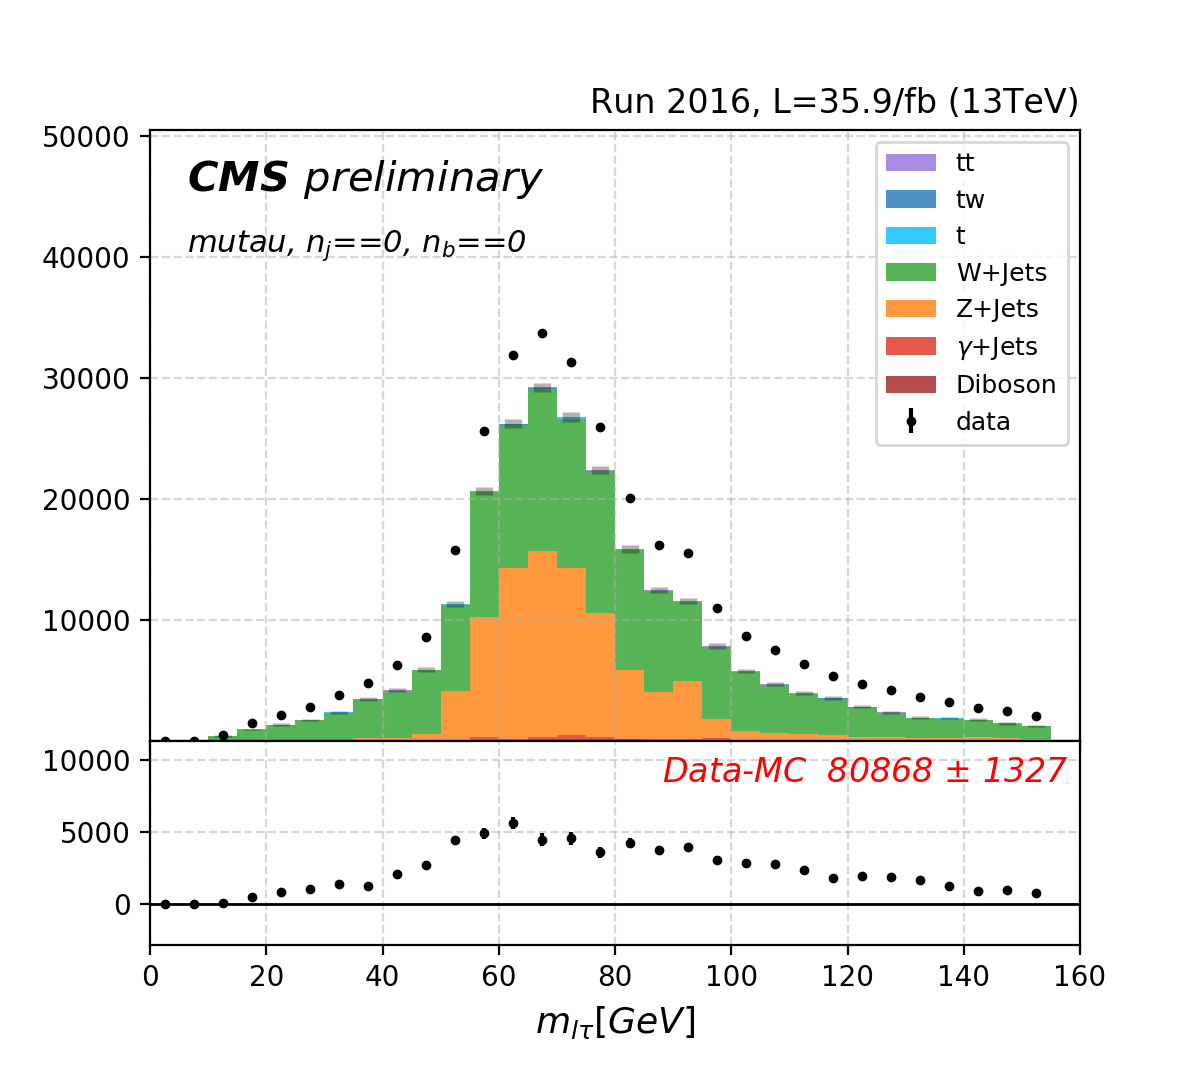
\includegraphics[width=0.24\textwidth]{chapters/Appendix/sectionQCD/figures/mutau_==0_==0_dilepton_mass.png}
    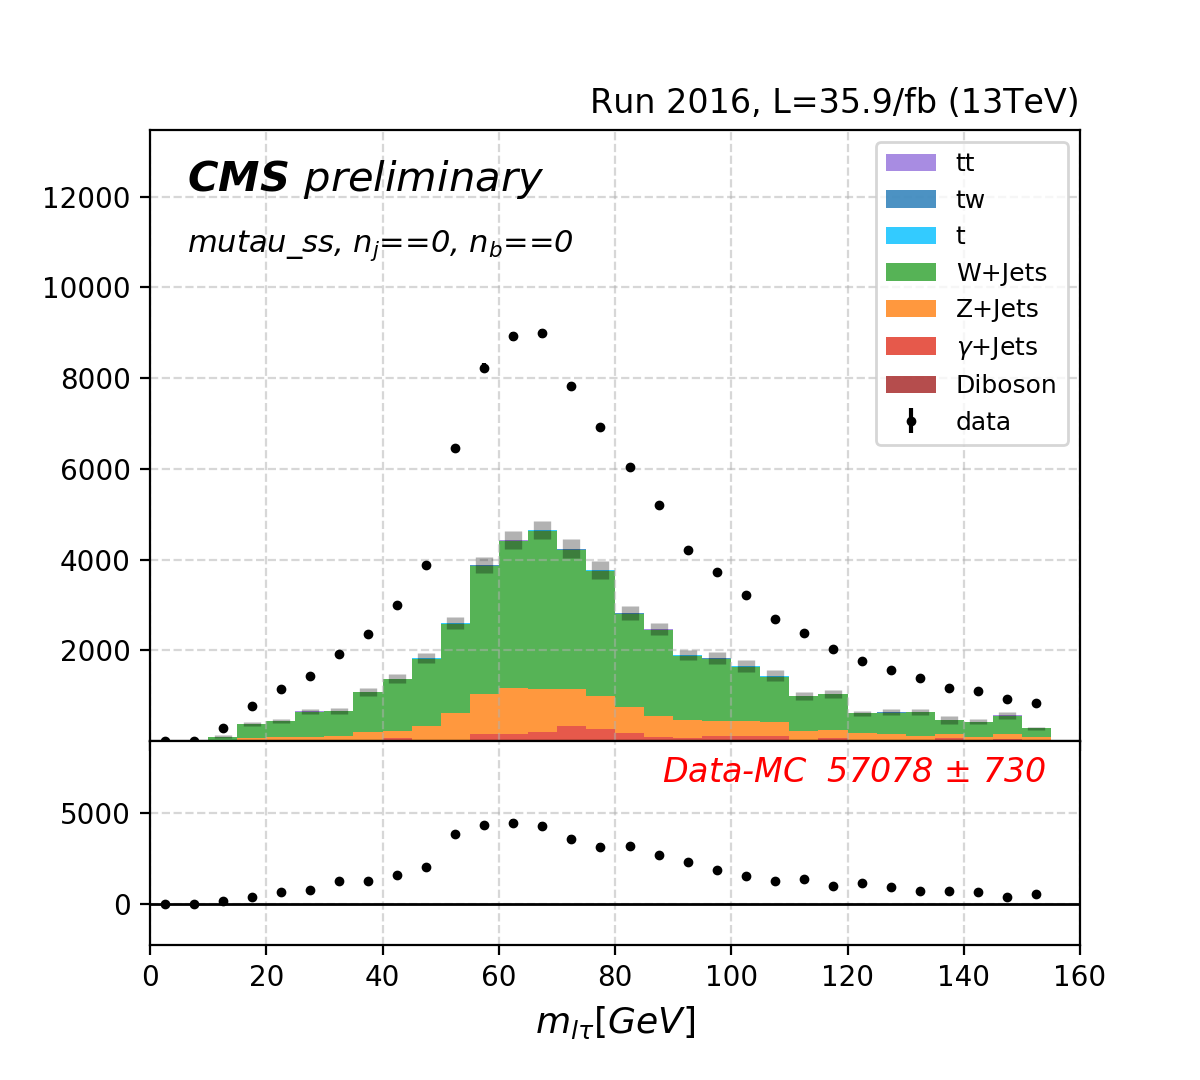
\includegraphics[width=0.24\textwidth]{chapters/Appendix/sectionQCD/figures/mutau_ss_==0_==0_dilepton_mass.png}
    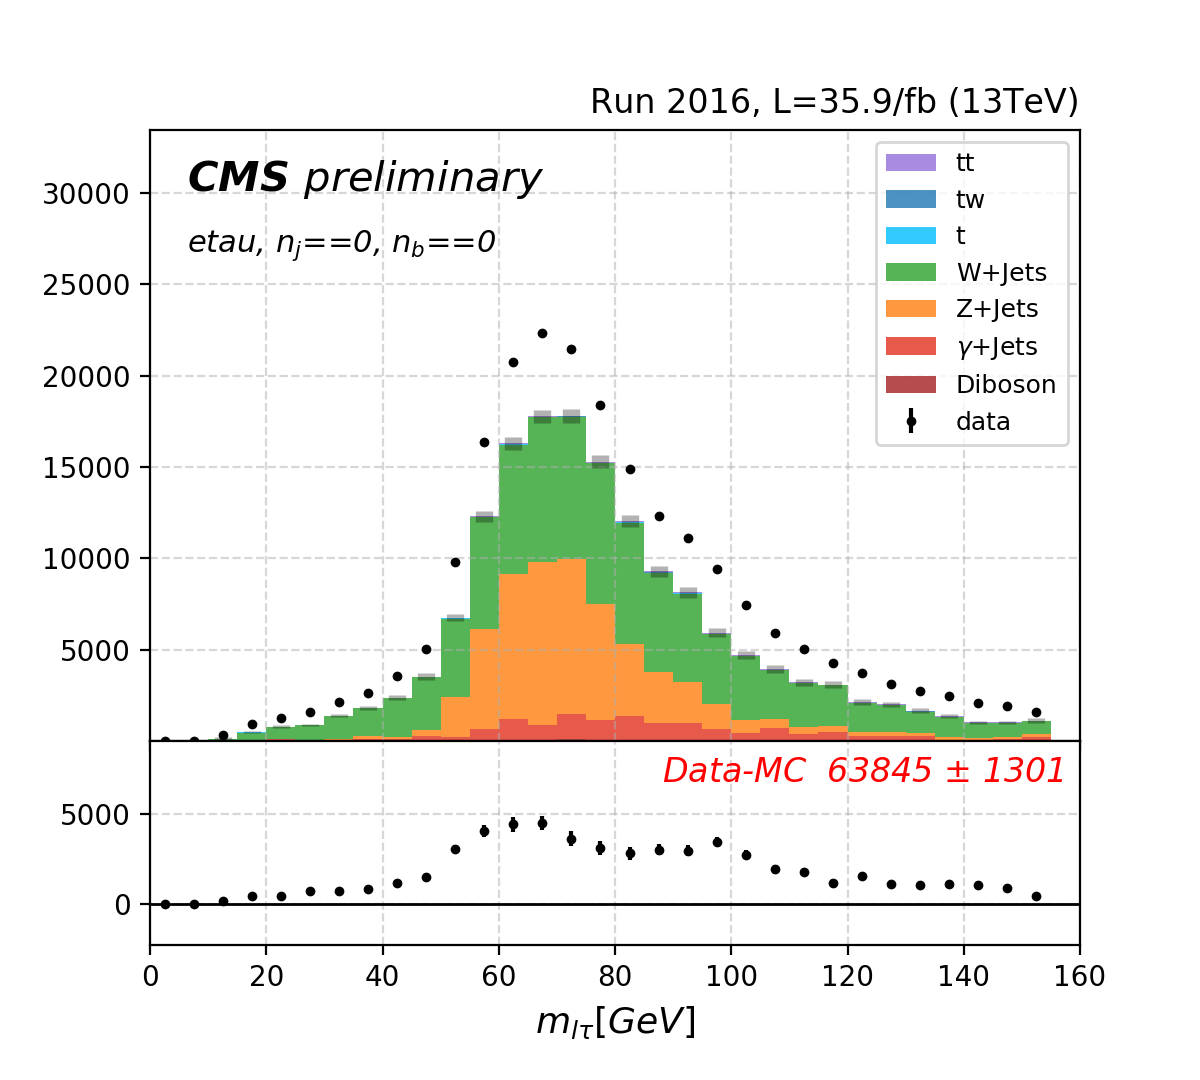
\includegraphics[width=0.24\textwidth]{chapters/Appendix/sectionQCD/figures/etau_==0_==0_dilepton_mass.png}
    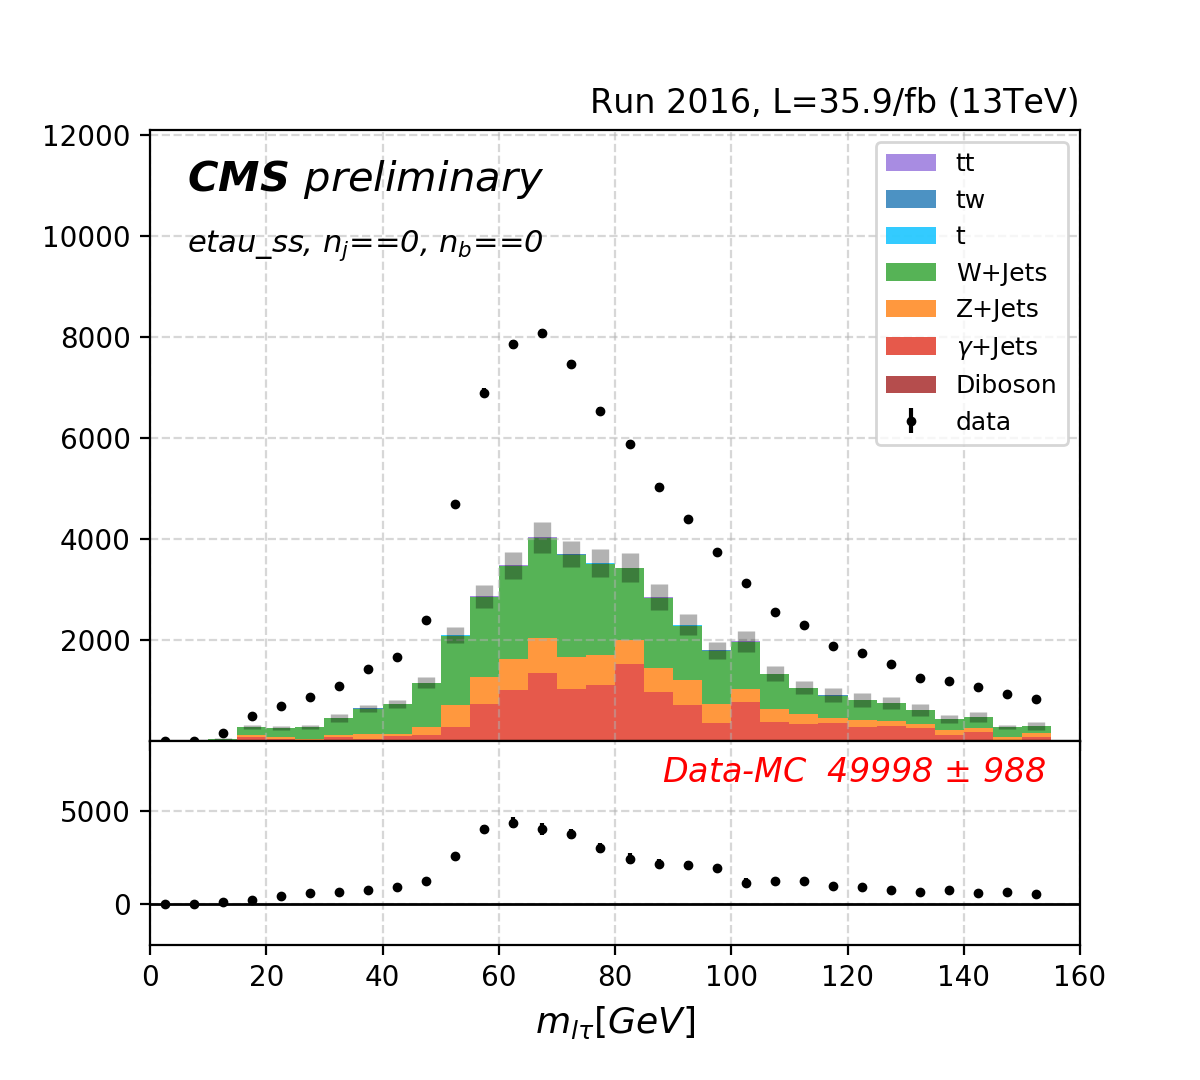
\includegraphics[width=0.24\textwidth]{chapters/Appendix/sectionQCD/figures/etau_ss_==0_==0_dilepton_mass.png}
    
    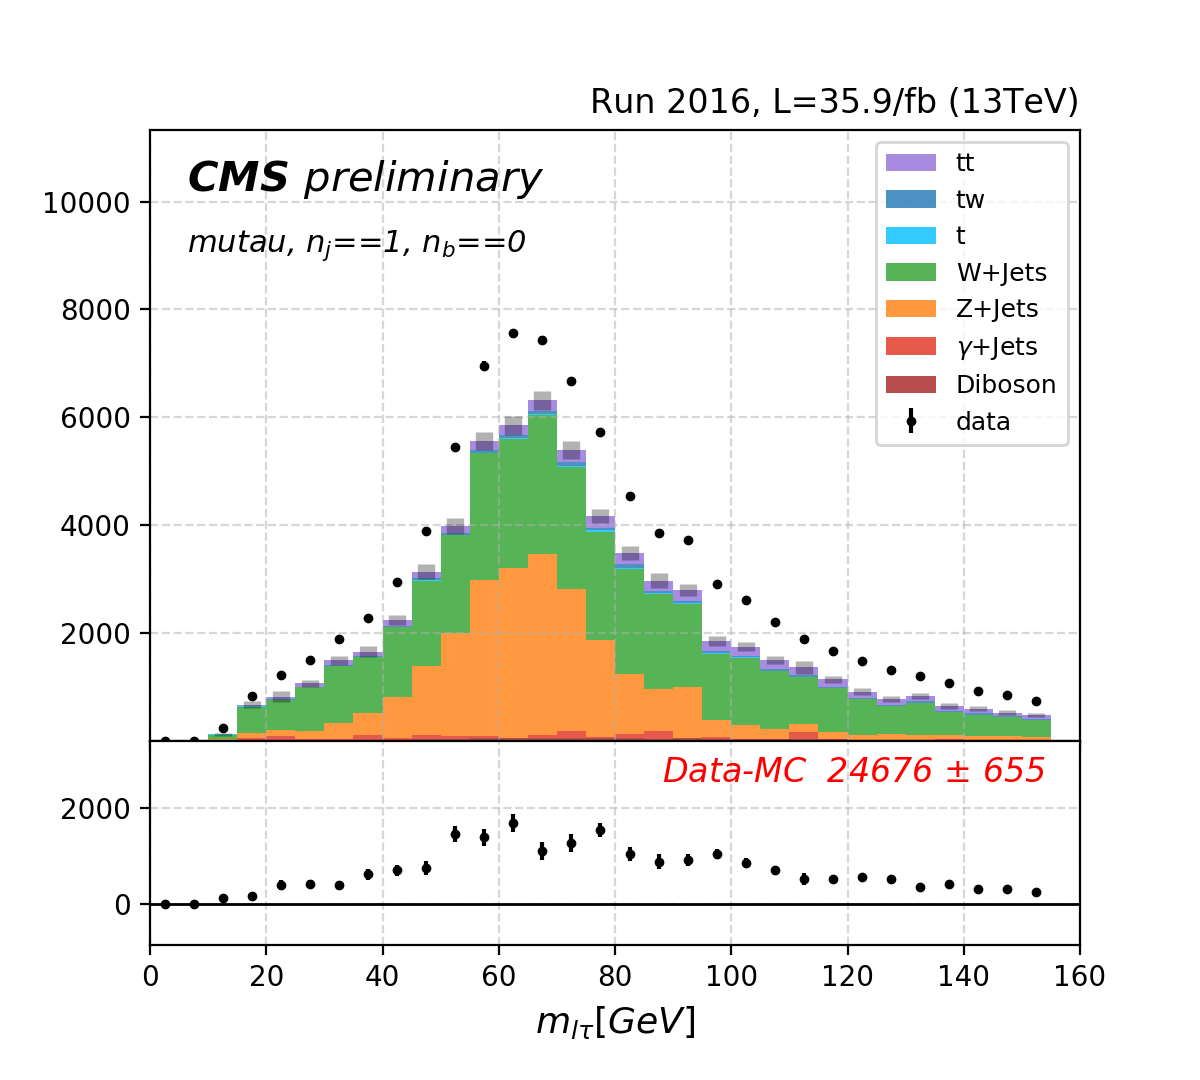
\includegraphics[width=0.24\textwidth]{chapters/Appendix/sectionQCD/figures/mutau_==1_==0_dilepton_mass.png}
    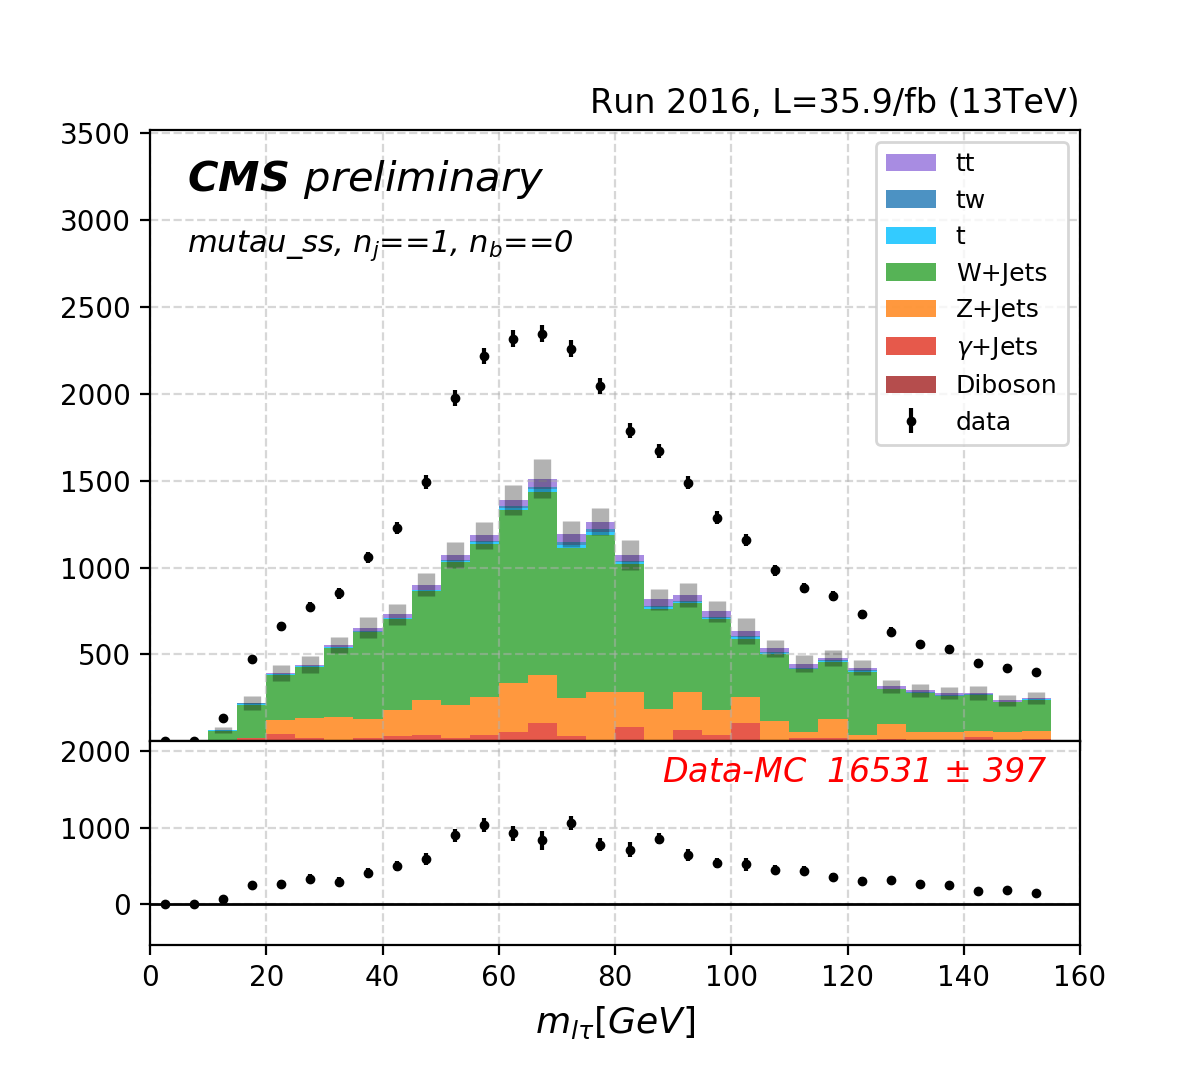
\includegraphics[width=0.24\textwidth]{chapters/Appendix/sectionQCD/figures/mutau_ss_==1_==0_dilepton_mass.png}
    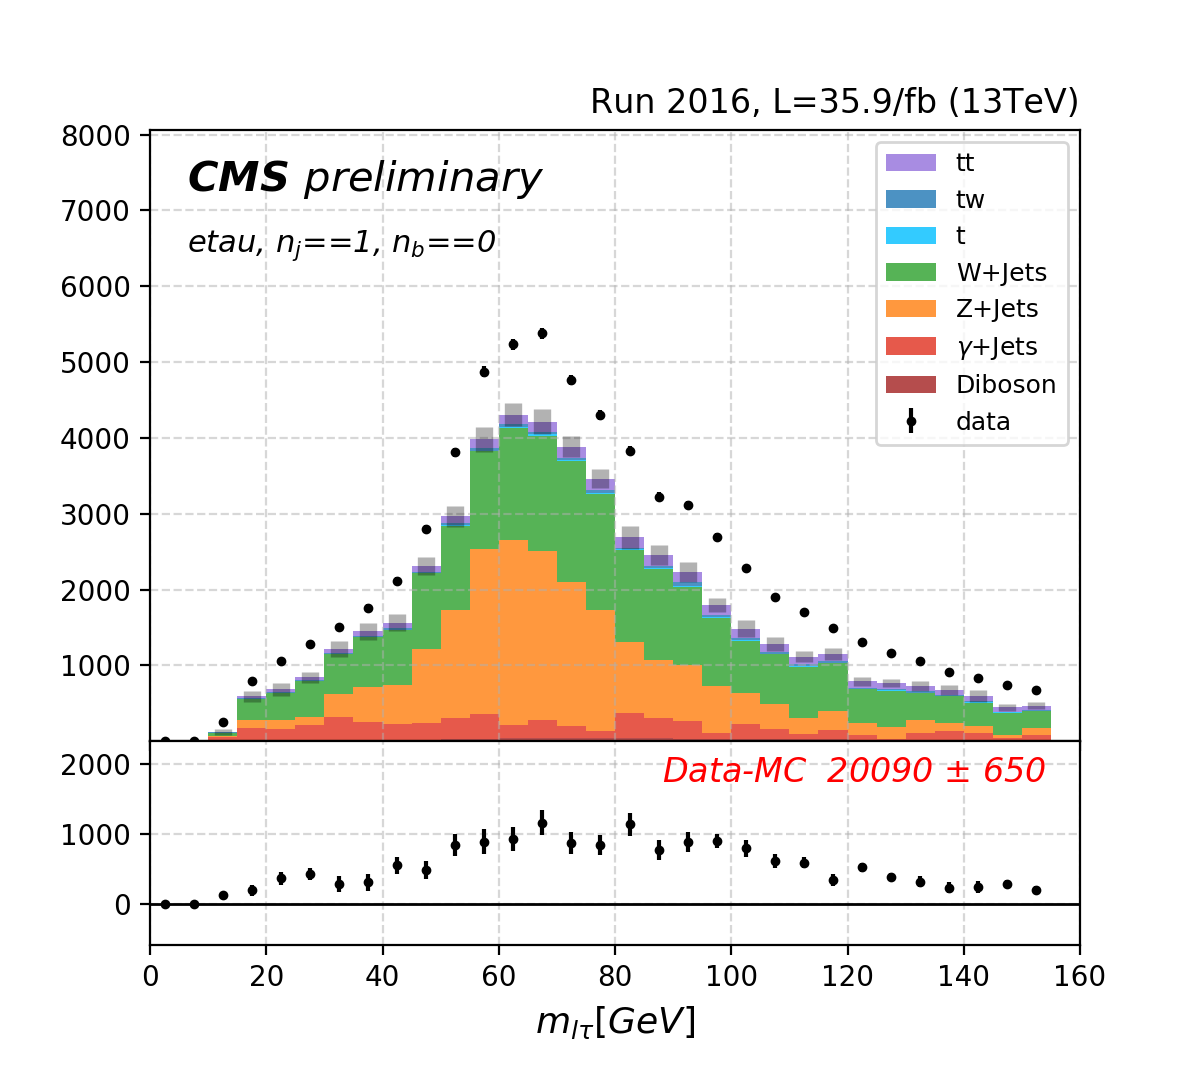
\includegraphics[width=0.24\textwidth]{chapters/Appendix/sectionQCD/figures/etau_==1_==0_dilepton_mass.png}
    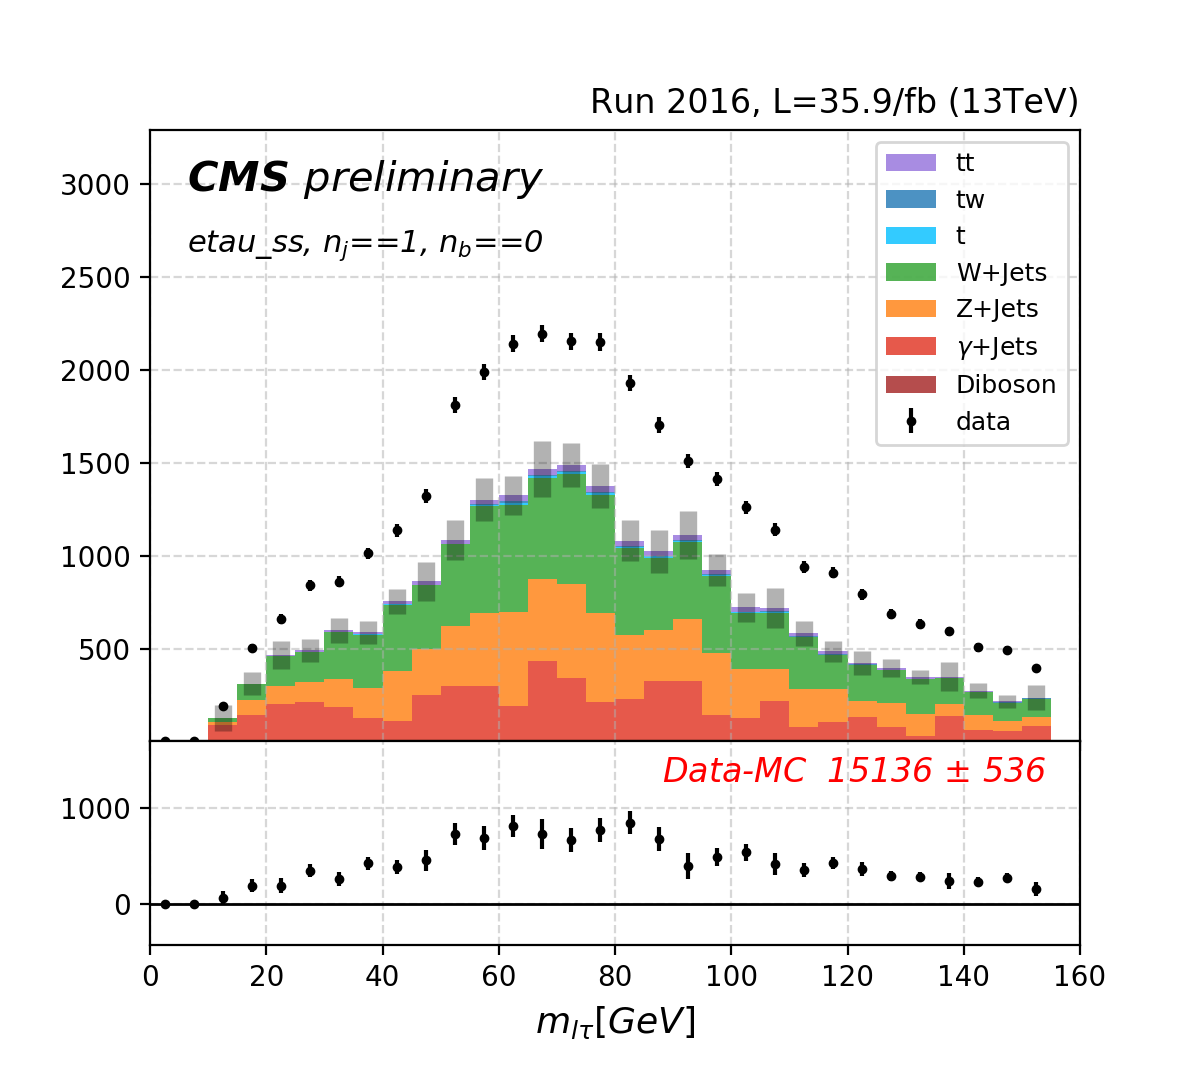
\includegraphics[width=0.24\textwidth]{chapters/Appendix/sectionQCD/figures/etau_ss_==1_==0_dilepton_mass.png}
    
    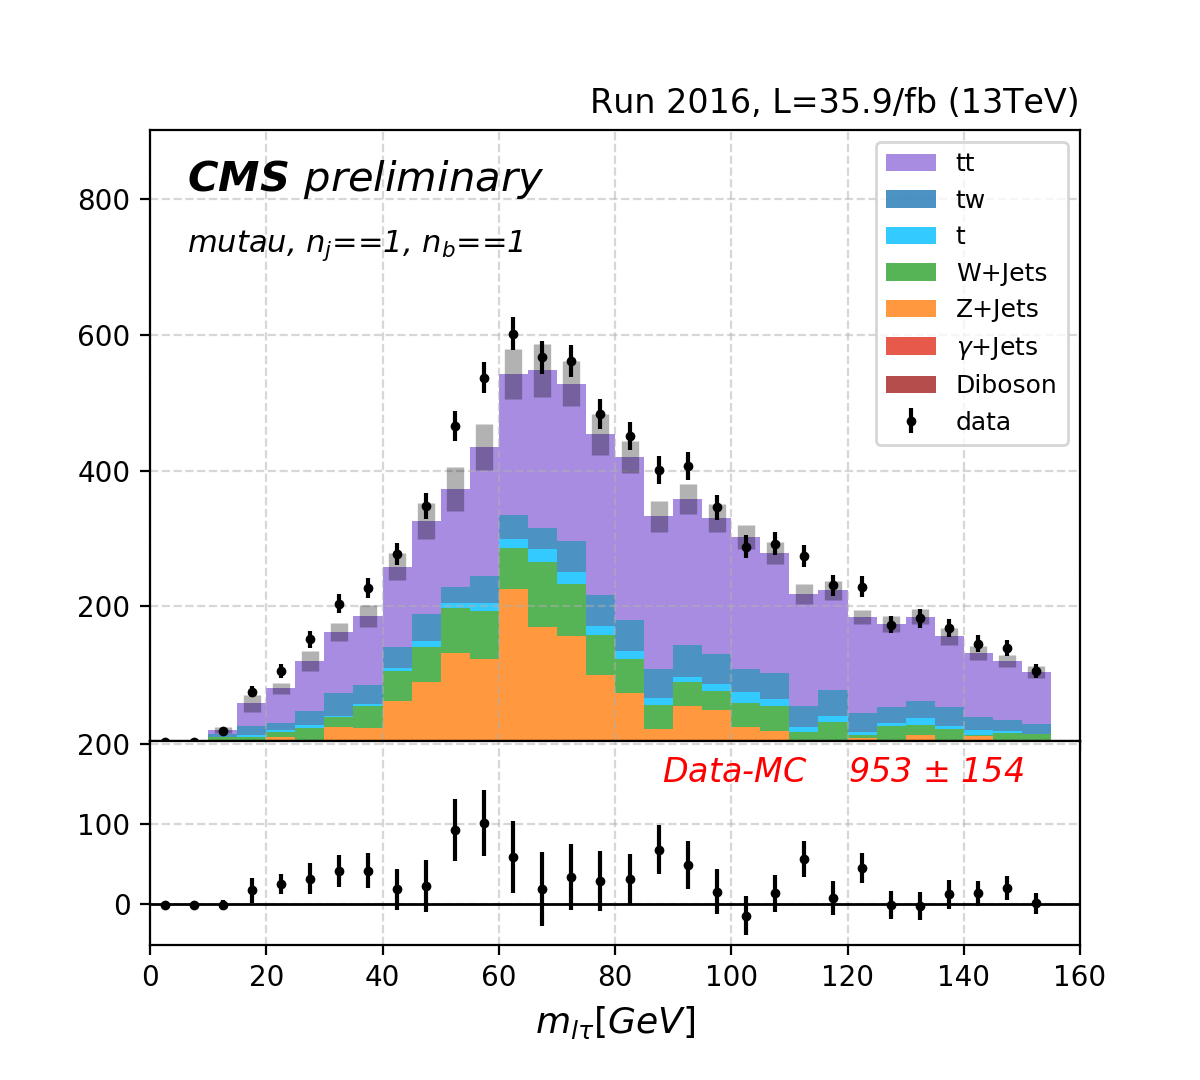
\includegraphics[width=0.24\textwidth]{chapters/Appendix/sectionQCD/figures/mutau_==1_==1_dilepton_mass.png}
    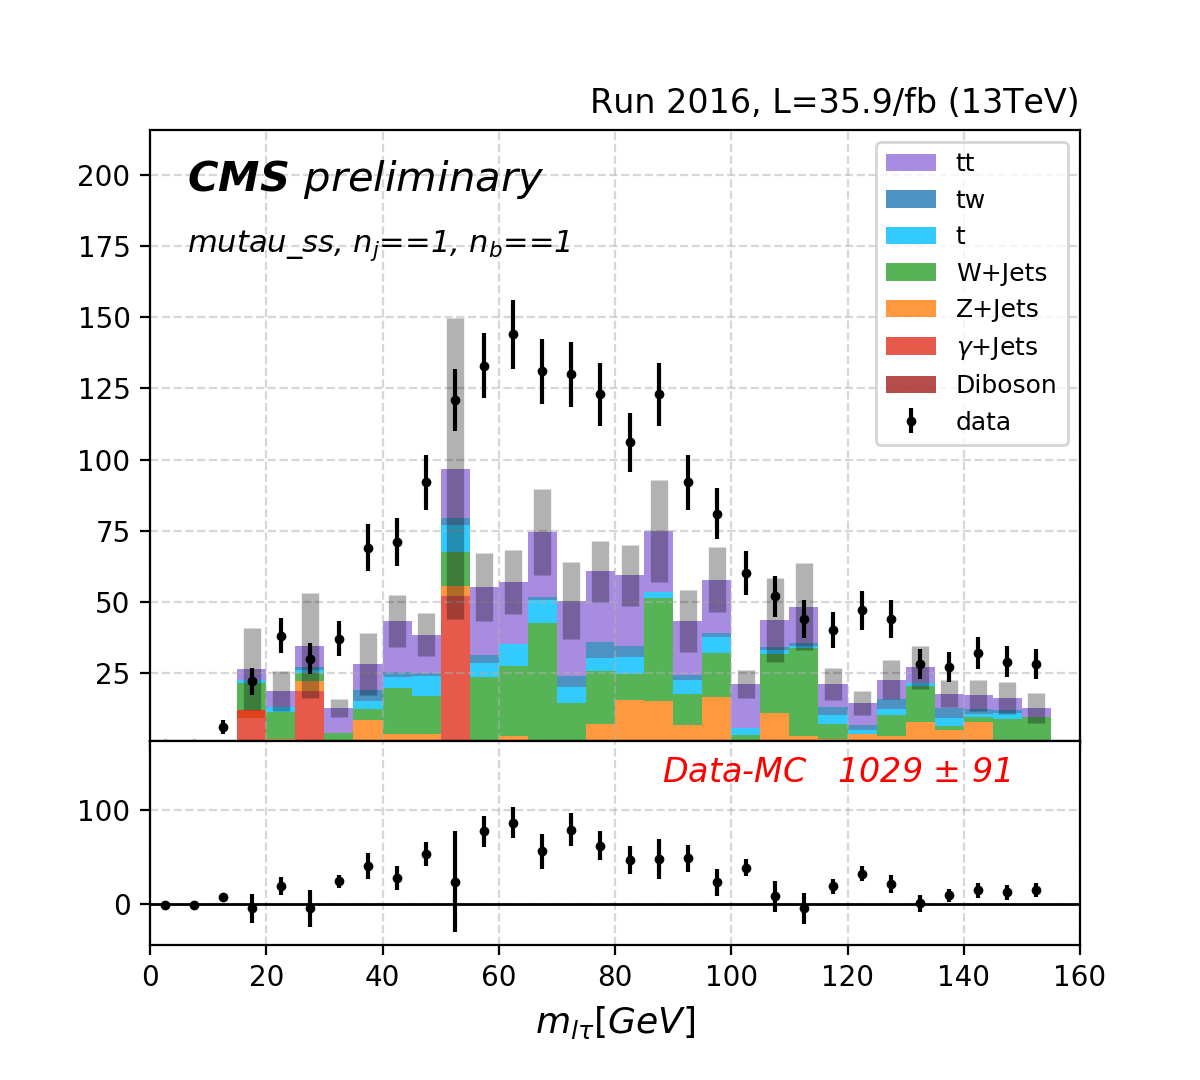
\includegraphics[width=0.24\textwidth]{chapters/Appendix/sectionQCD/figures/mutau_ss_==1_==1_dilepton_mass.png}
    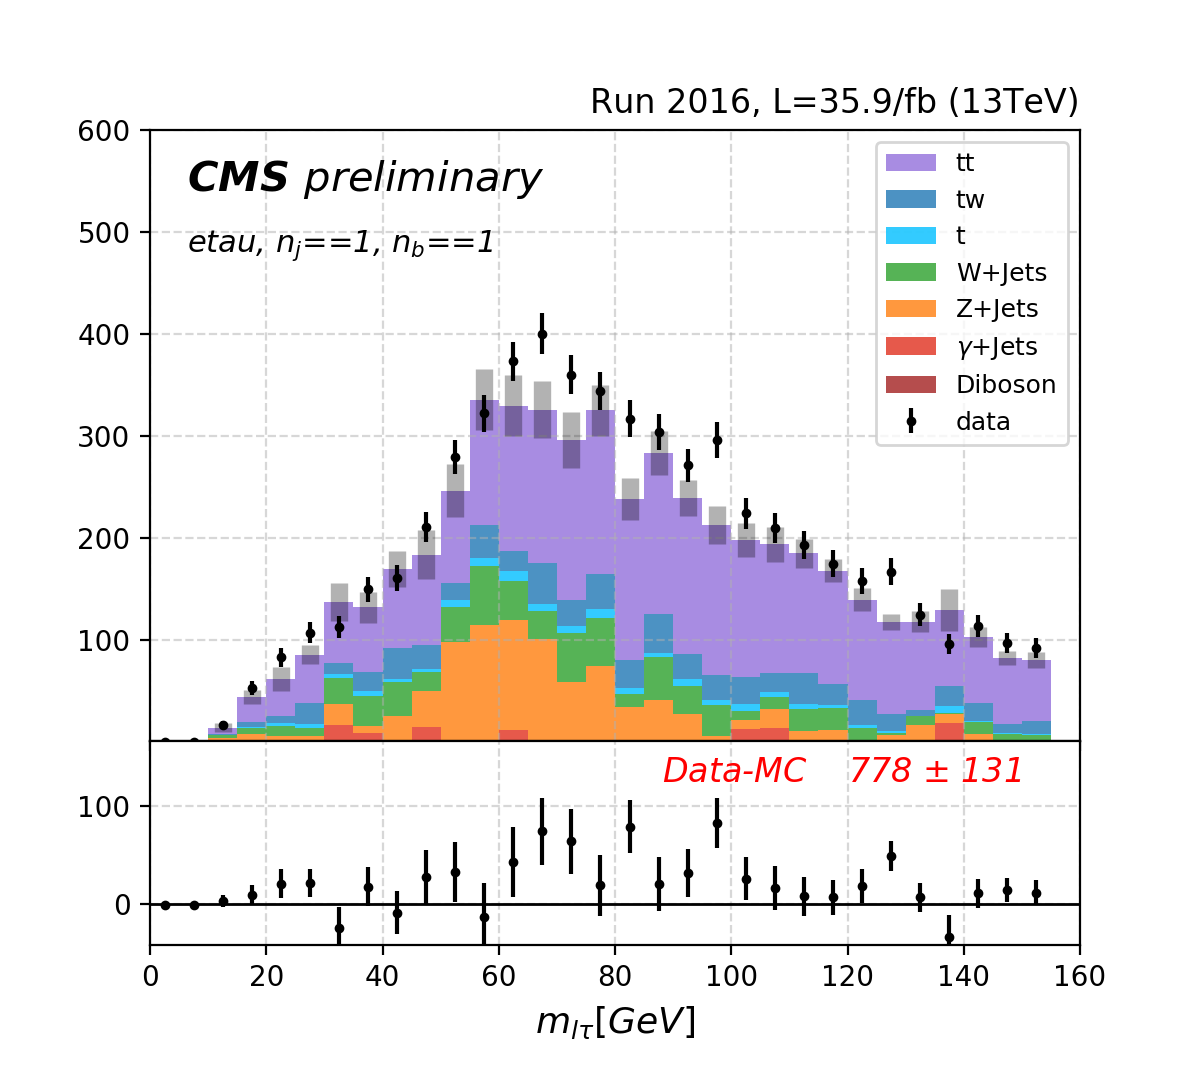
\includegraphics[width=0.24\textwidth]{chapters/Appendix/sectionQCD/figures/etau_==1_==1_dilepton_mass.png}
    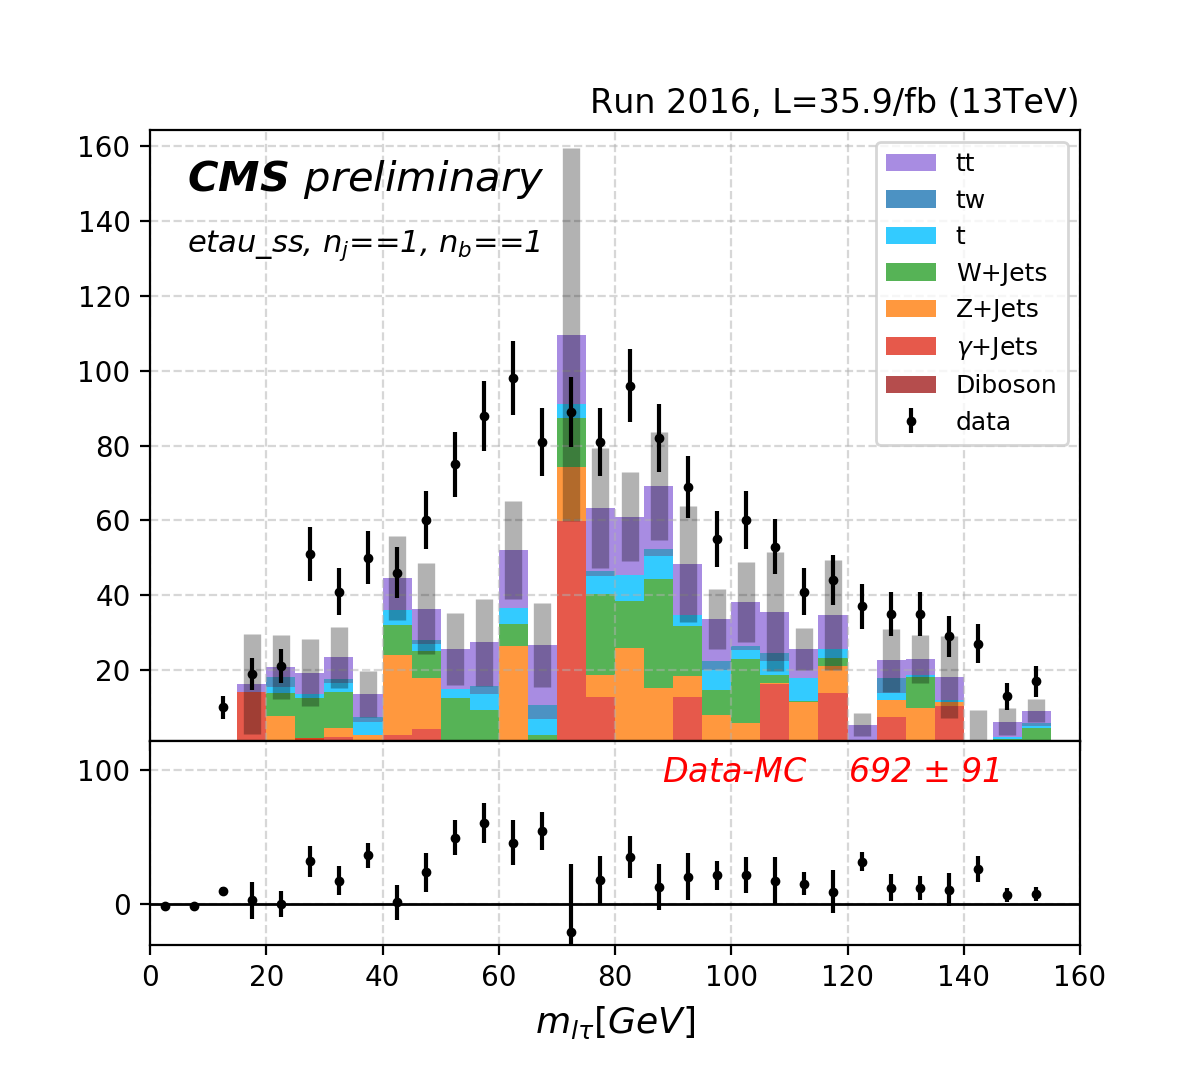
\includegraphics[width=0.24\textwidth]{chapters/Appendix/sectionQCD/figures/etau_ss_==1_==1_dilepton_mass.png}
    
    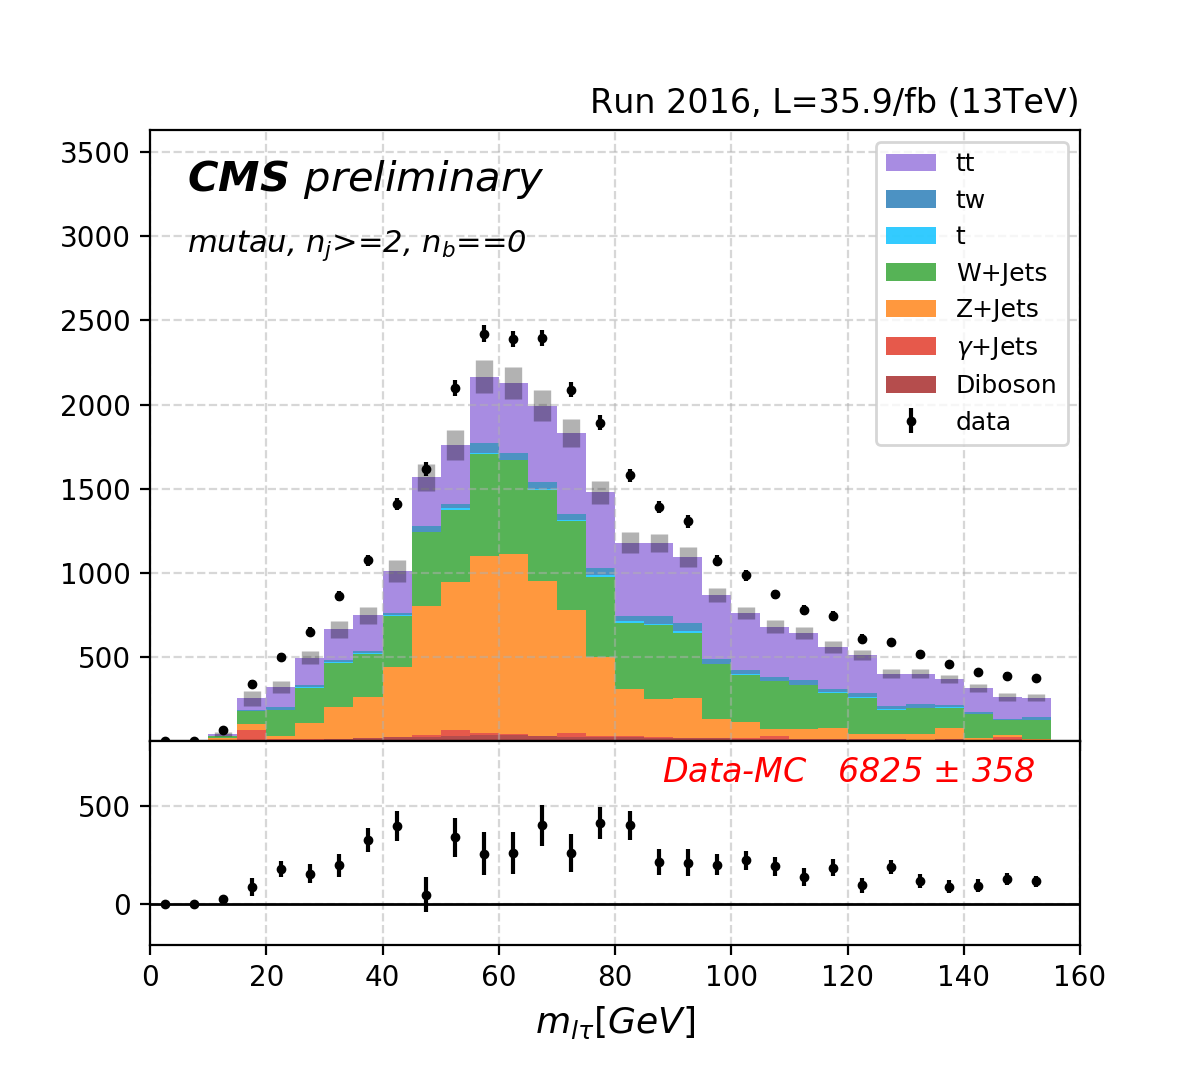
\includegraphics[width=0.24\textwidth]{chapters/Appendix/sectionQCD/figures/mutau_>=2_==0_dilepton_mass.png}
    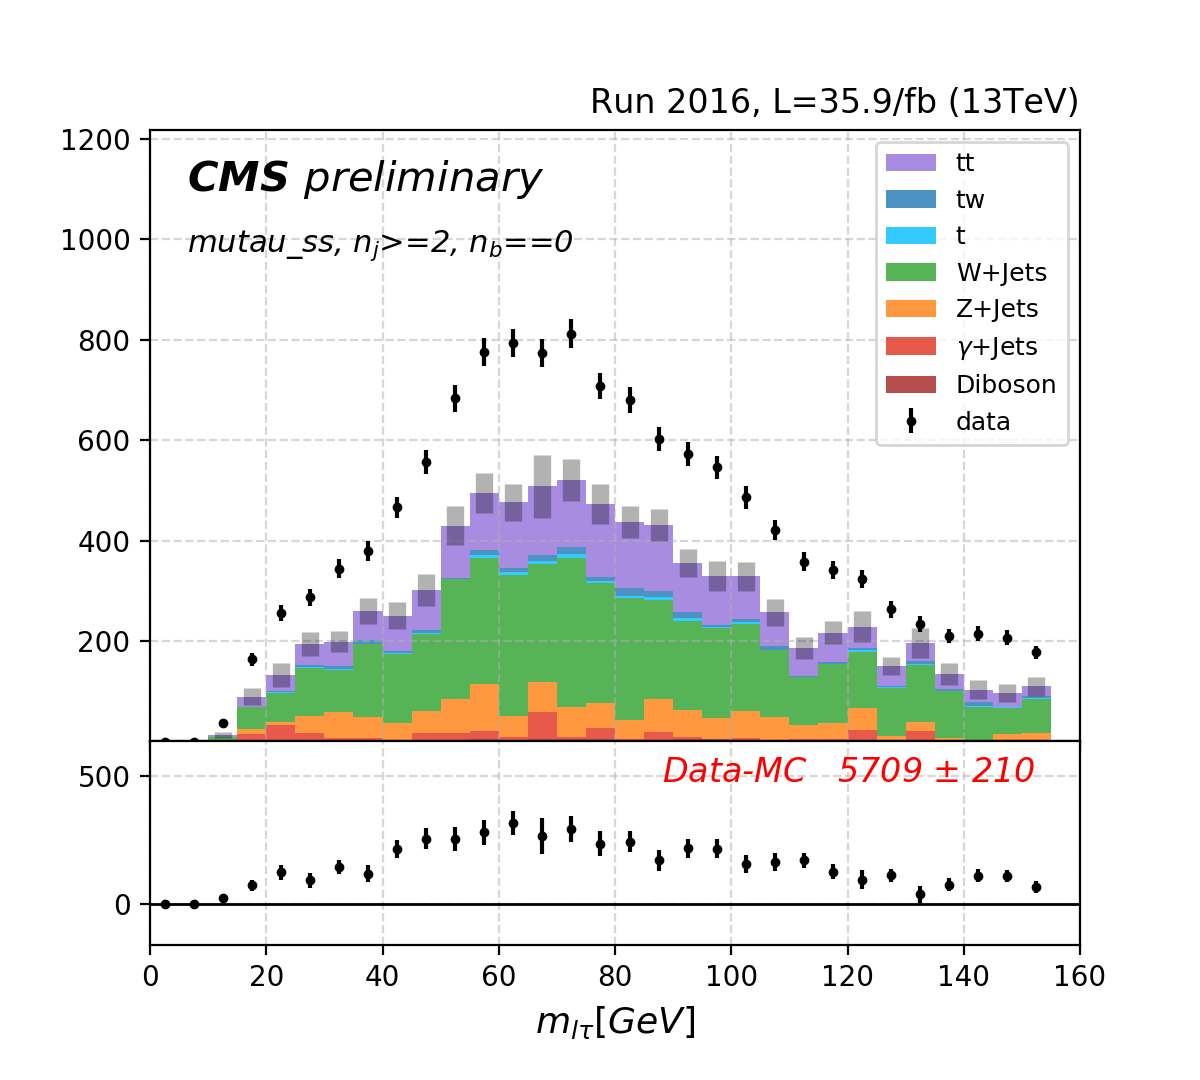
\includegraphics[width=0.24\textwidth]{chapters/Appendix/sectionQCD/figures/mutau_ss_>=2_==0_dilepton_mass.png}
    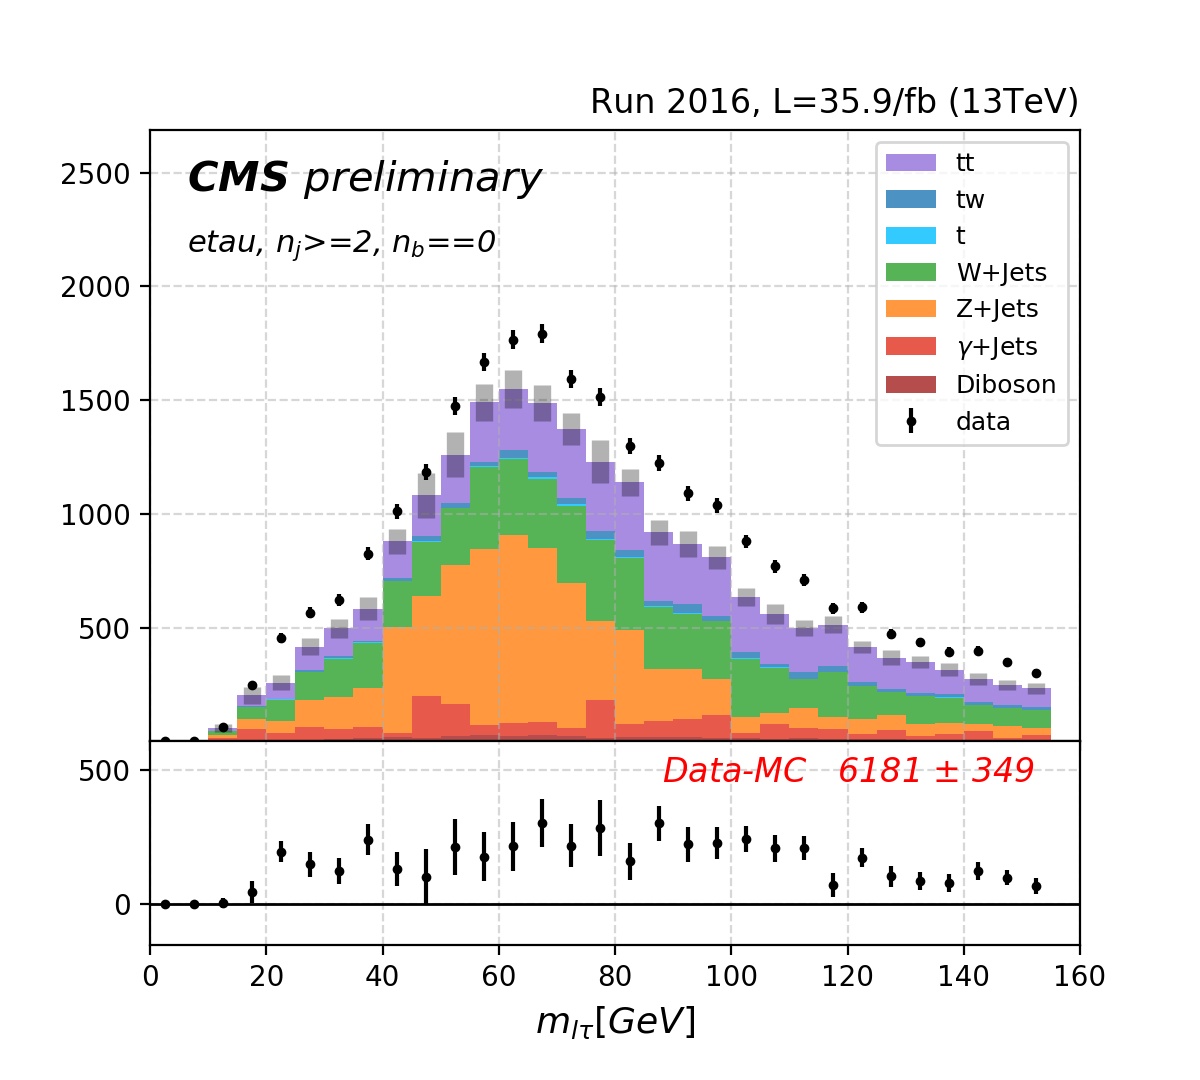
\includegraphics[width=0.24\textwidth]{chapters/Appendix/sectionQCD/figures/etau_>=2_==0_dilepton_mass.png}
    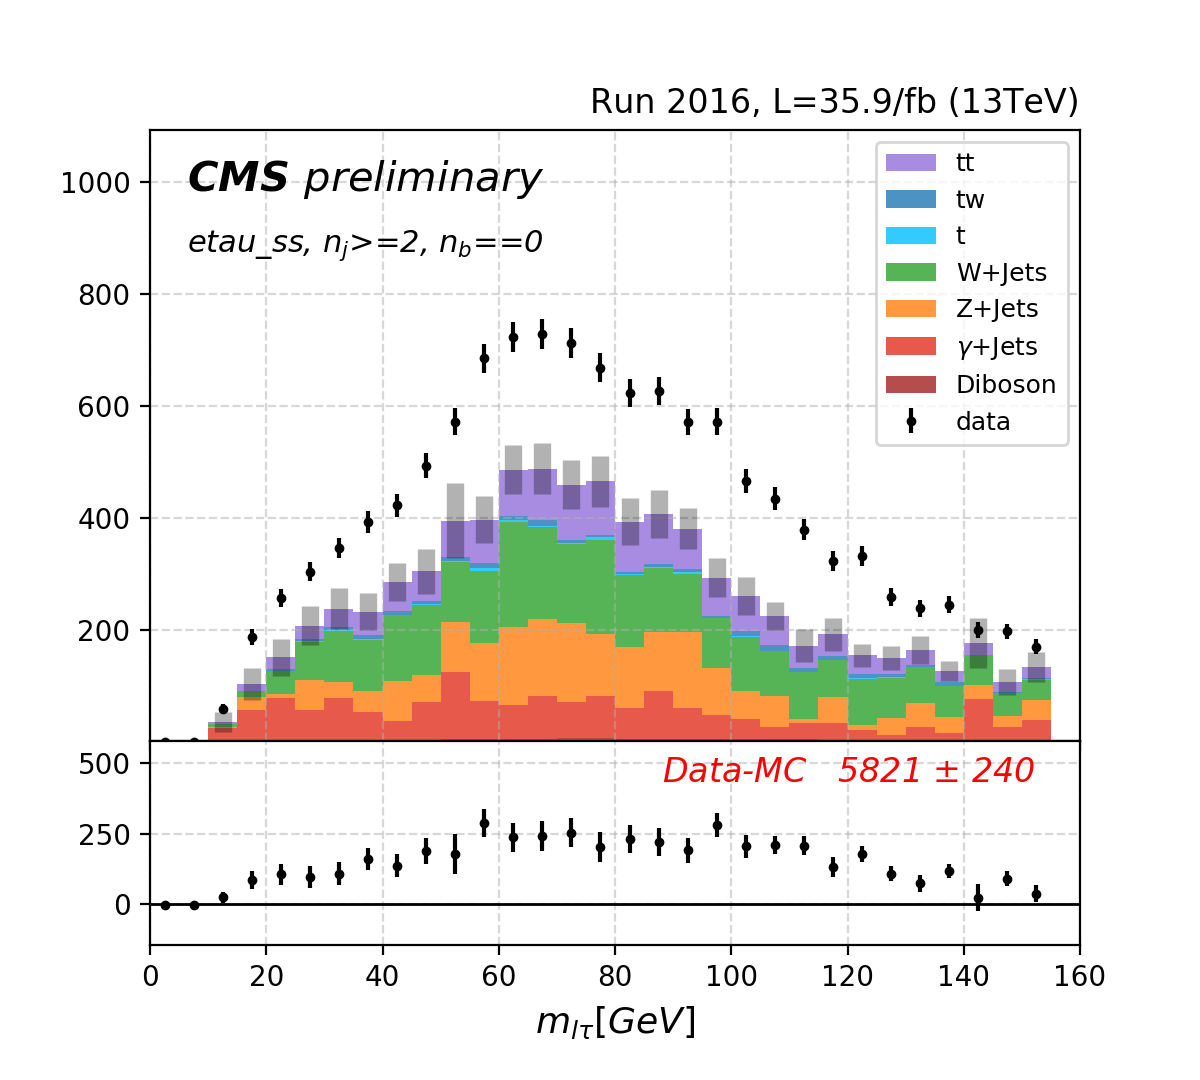
\includegraphics[width=0.24\textwidth]{chapters/Appendix/sectionQCD/figures/etau_ss_>=2_==0_dilepton_mass.png}
    
    
    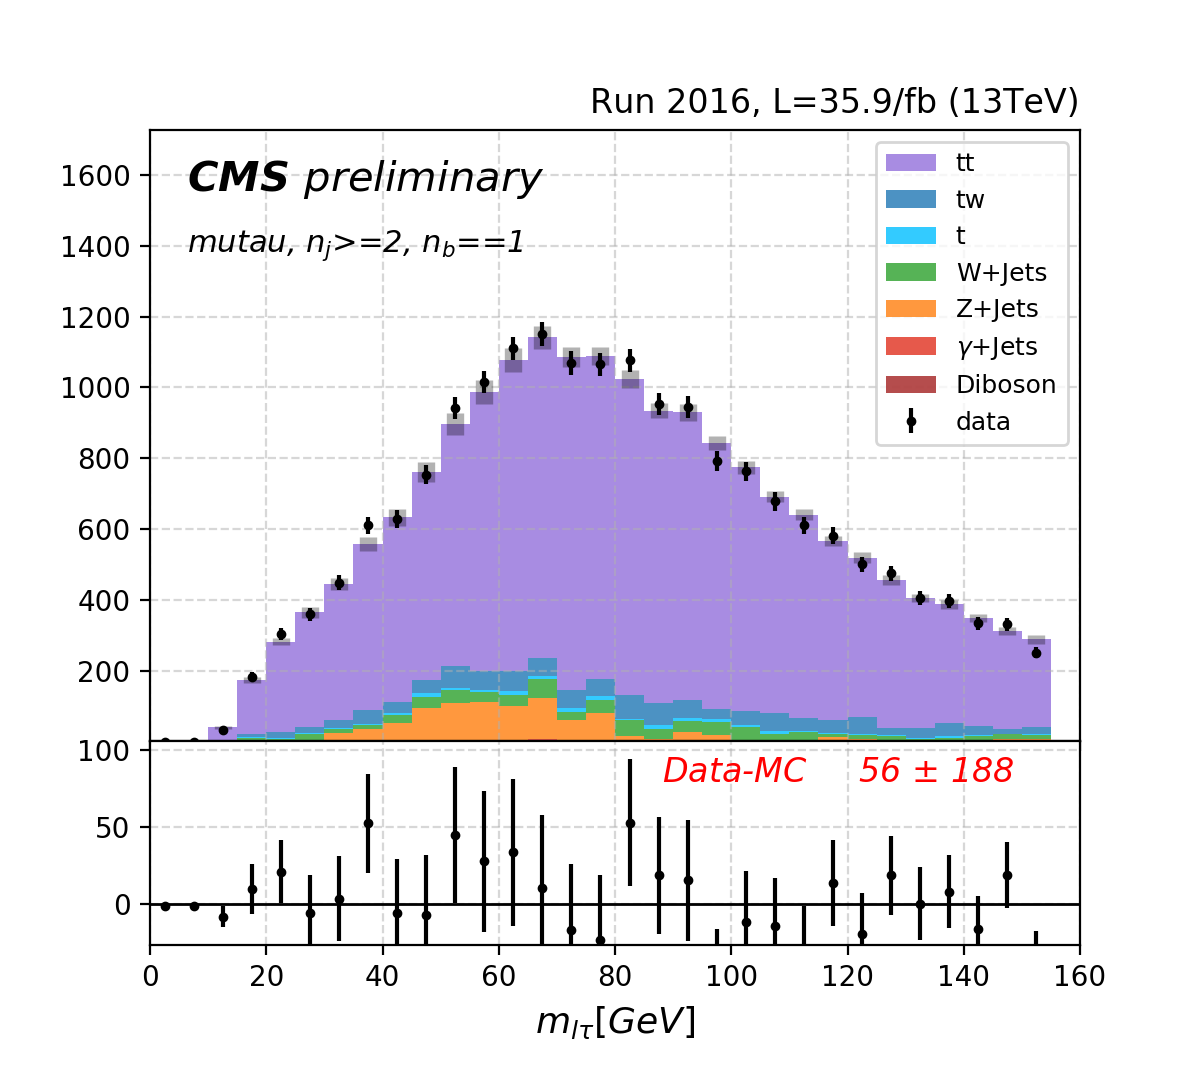
\includegraphics[width=0.24\textwidth]{chapters/Appendix/sectionQCD/figures/mutau_>=2_==1_dilepton_mass.png}
    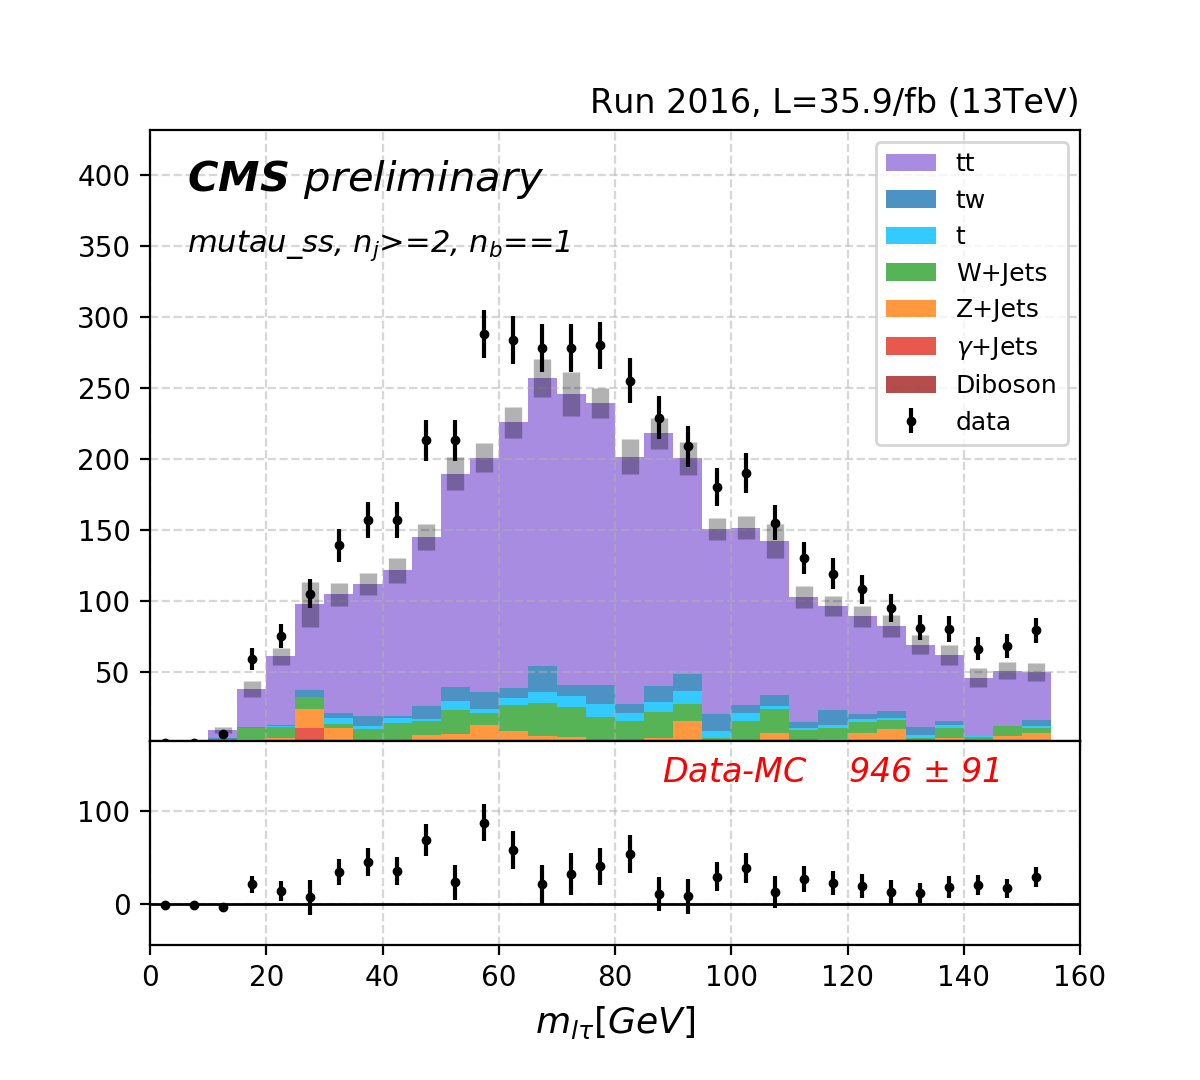
\includegraphics[width=0.24\textwidth]{chapters/Appendix/sectionQCD/figures/mutau_ss_>=2_==1_dilepton_mass.png}
    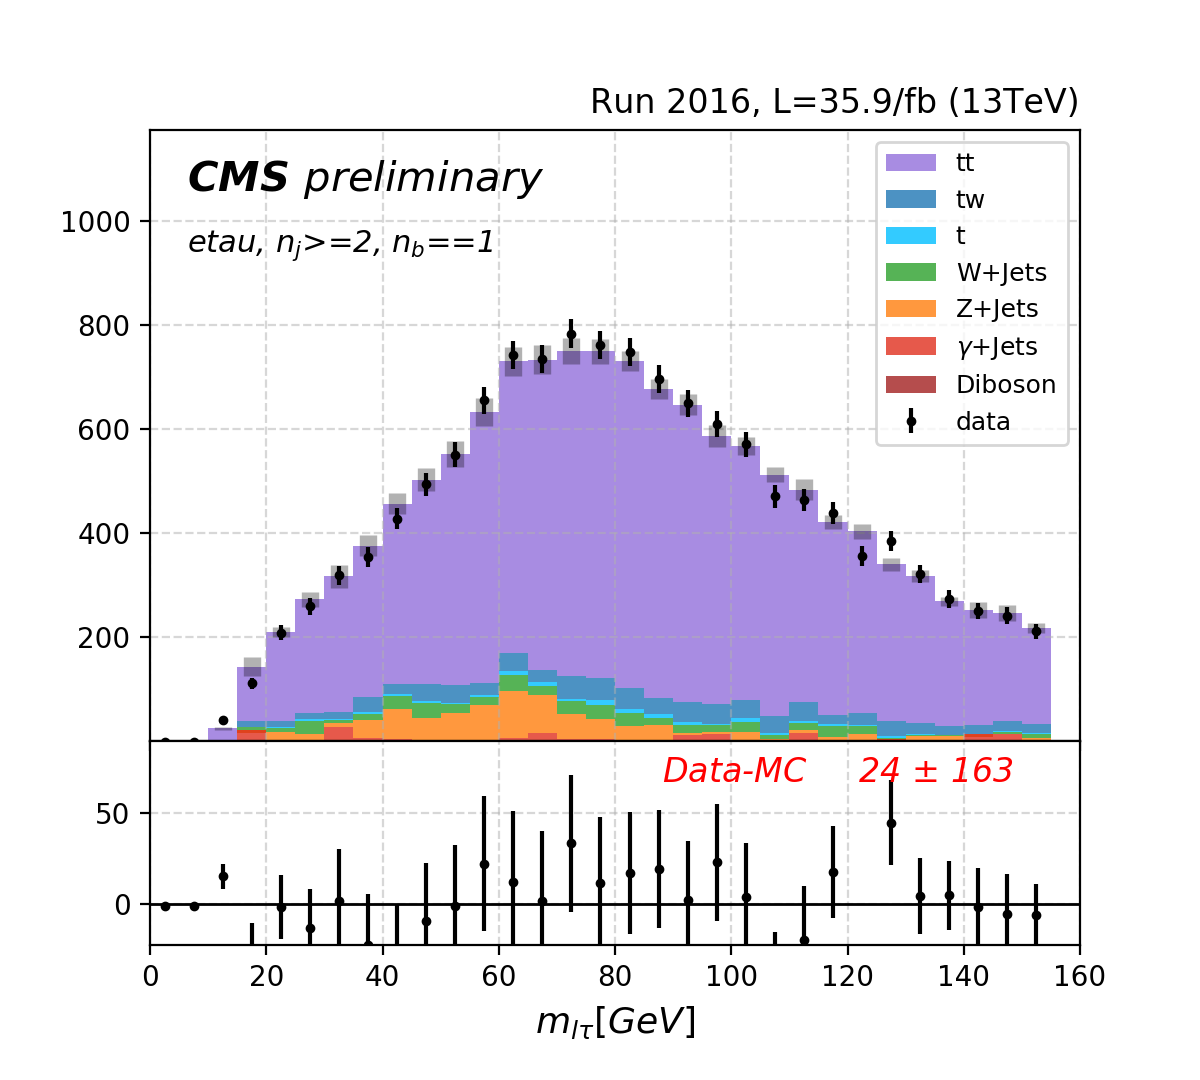
\includegraphics[width=0.24\textwidth]{chapters/Appendix/sectionQCD/figures/etau_>=2_==1_dilepton_mass.png}
    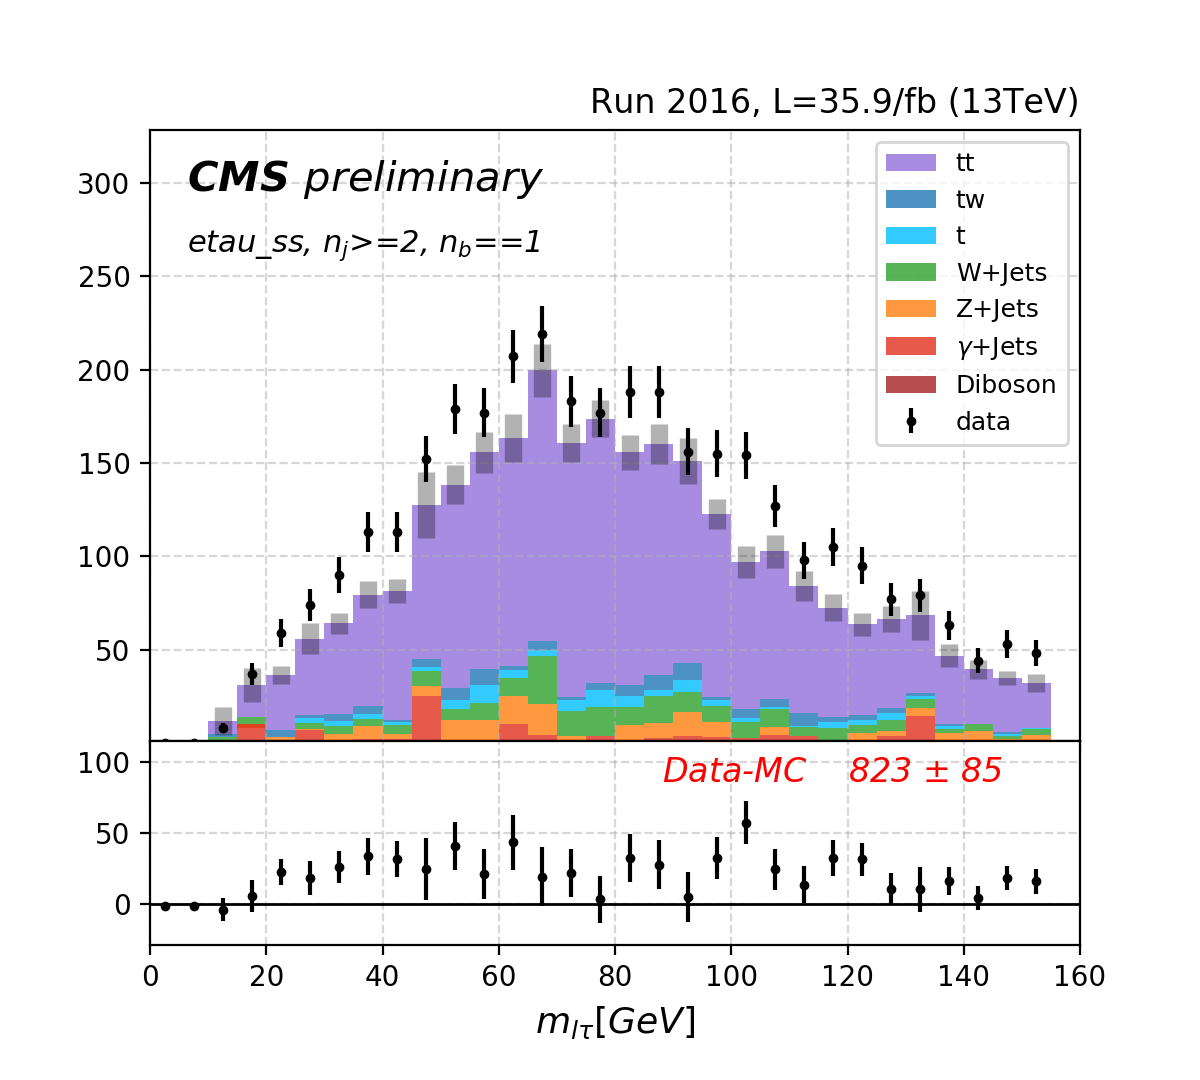
\includegraphics[width=0.24\textwidth]{chapters/Appendix/sectionQCD/figures/etau_ss_>=2_==1_dilepton_mass.png}
    
    
    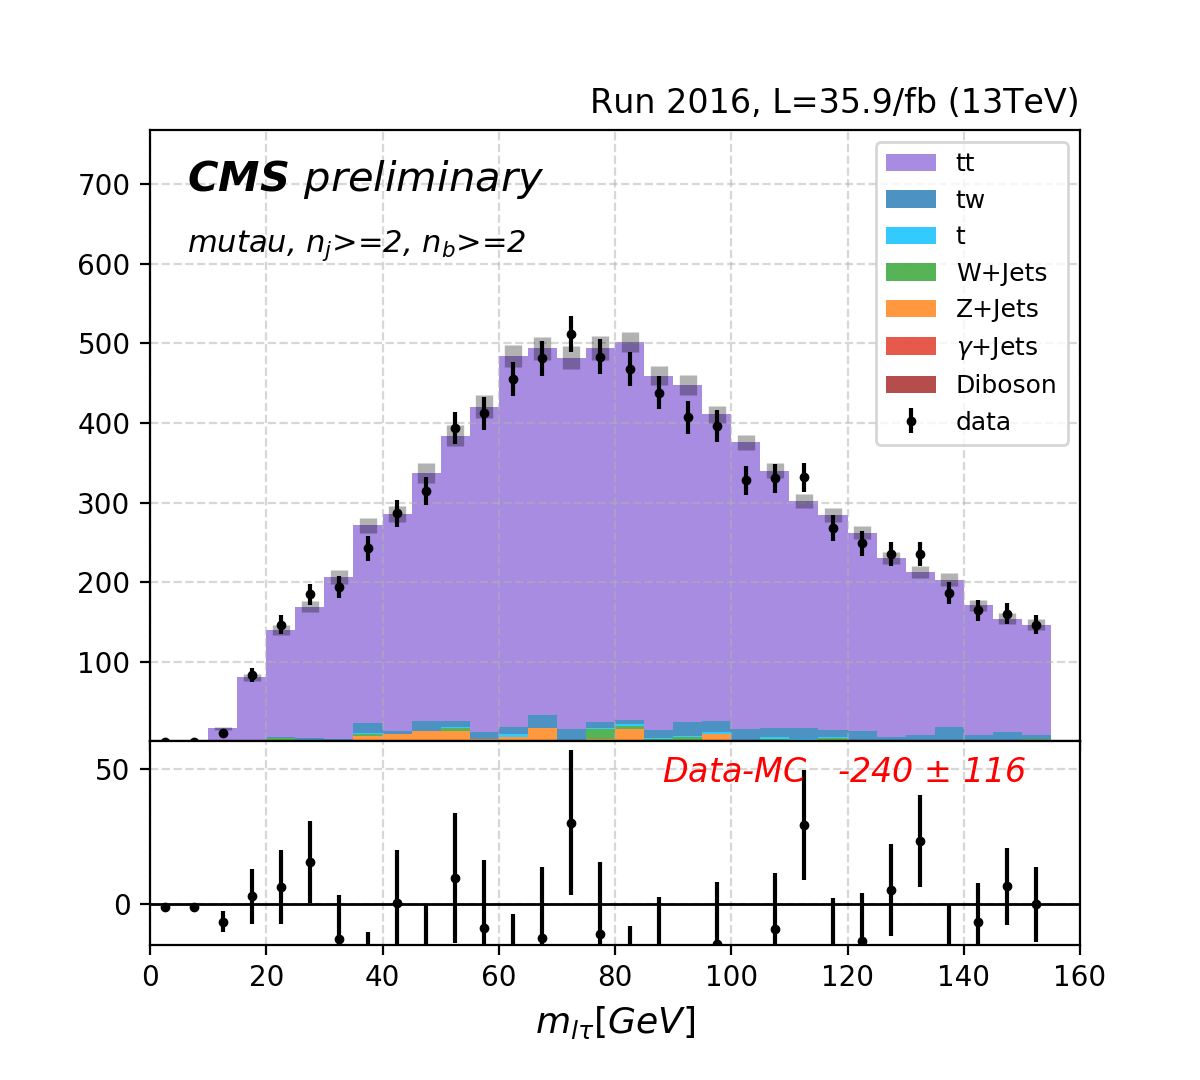
\includegraphics[width=0.24\textwidth]{chapters/Appendix/sectionQCD/figures/mutau_>=2_>=2_dilepton_mass.png}
    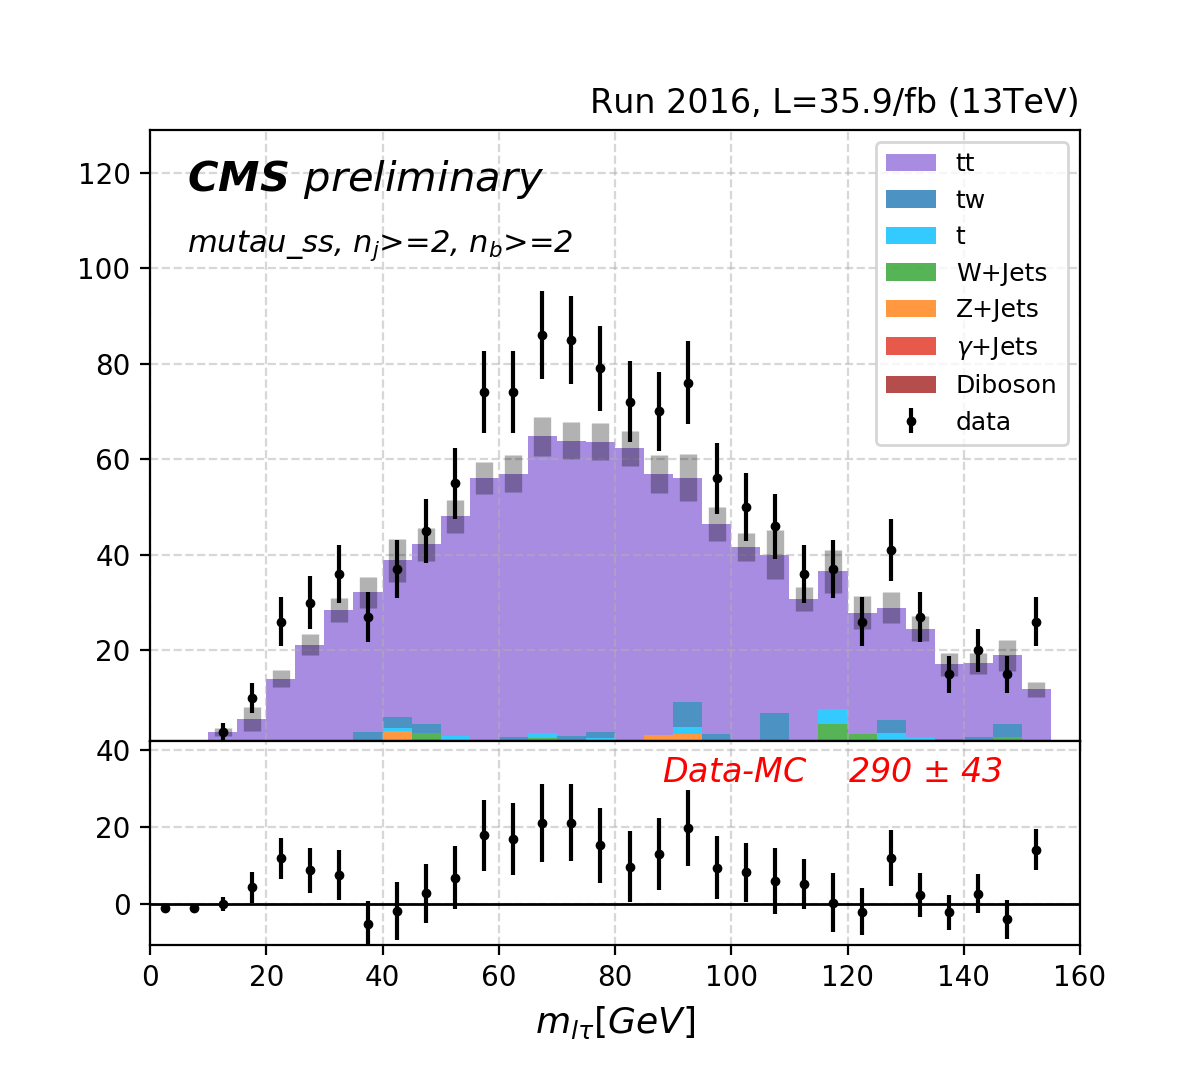
\includegraphics[width=0.24\textwidth]{chapters/Appendix/sectionQCD/figures/mutau_ss_>=2_>=2_dilepton_mass.png}
    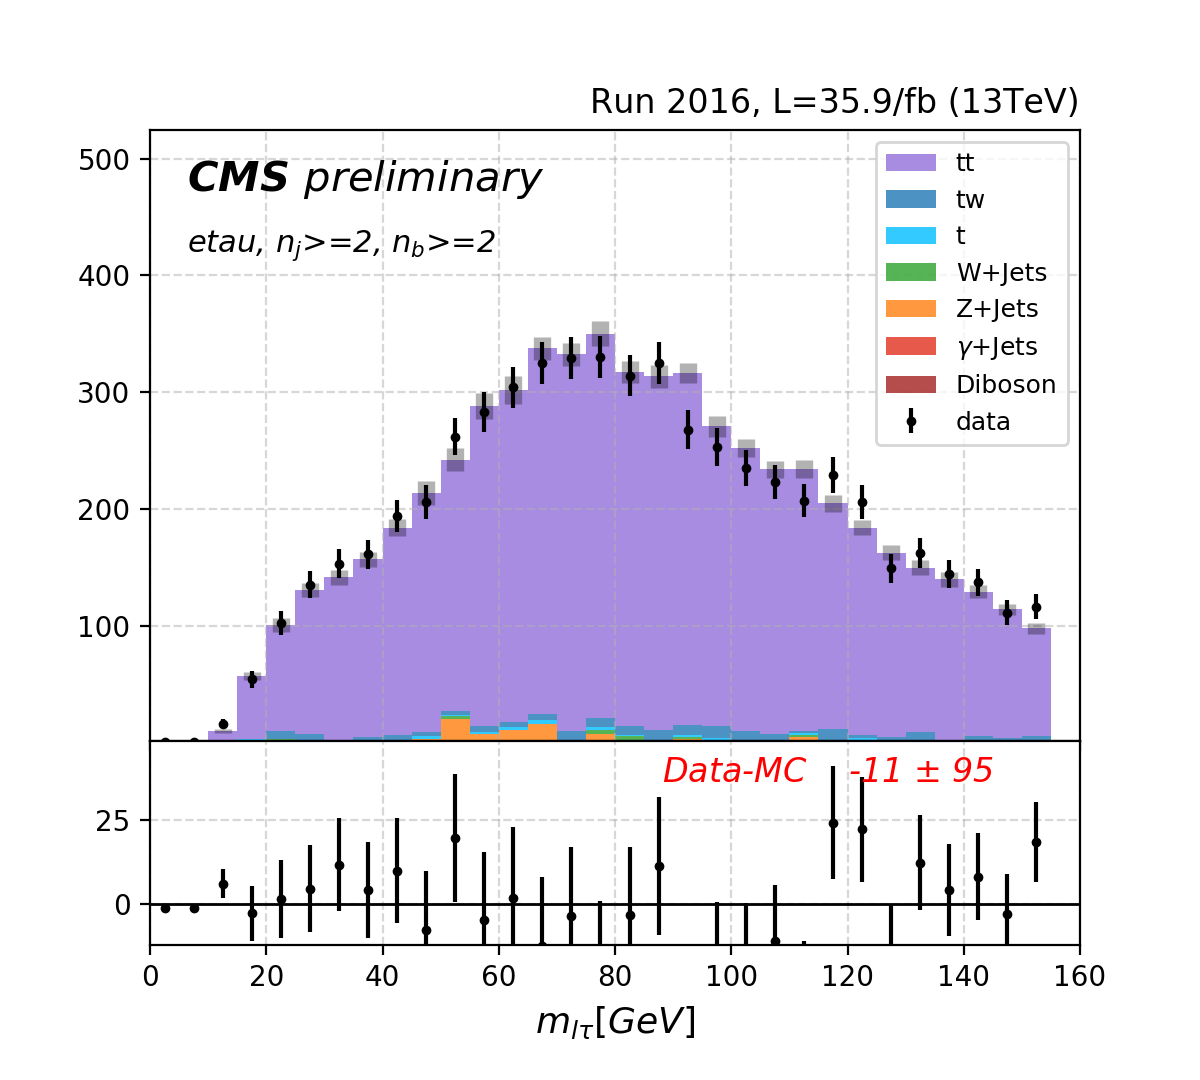
\includegraphics[width=0.24\textwidth]{chapters/Appendix/sectionQCD/figures/etau_>=2_>=2_dilepton_mass.png}
    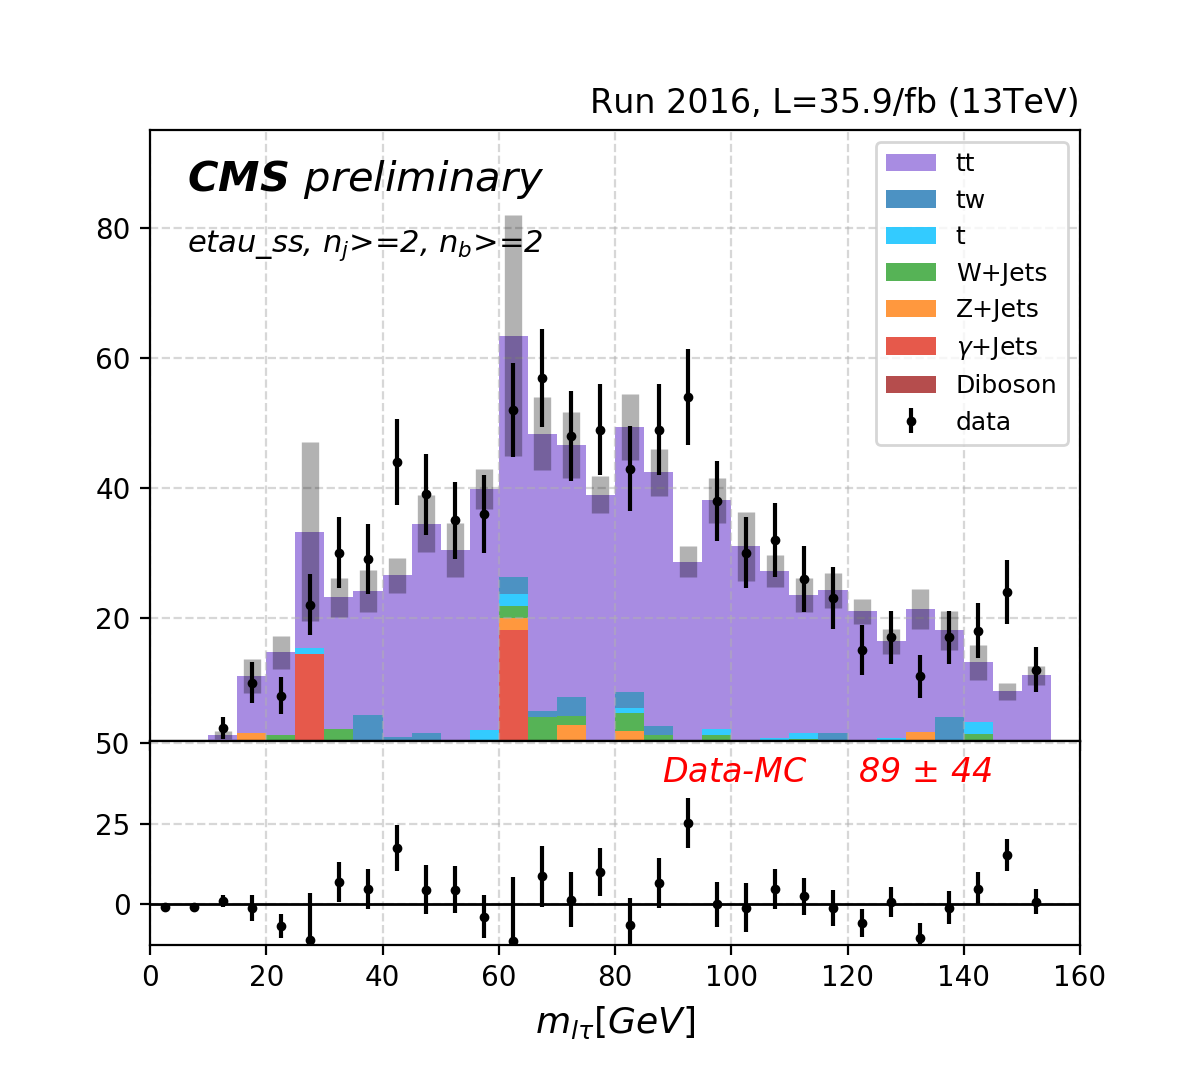
\includegraphics[width=0.24\textwidth]{chapters/Appendix/sectionQCD/figures/etau_ss_>=2_>=2_dilepton_mass.png}
    
    

    \caption{The $m_{l\tau}$ in the SS and OS region of $\mu\tau$ (left two columns) and $e\tau$ (right two columns) 
    channel. Different rows correspond to different $n_j,n_b$ configuration, which includes
    $n_j=0,n_b=0$, $n_j=1,n_b=0$, $n_j=1,n_b=1$, $n_j\geq 2,n_b=0$, $n_j\geq 2,n_b=1$, $n_j\geq 2,n_b\geq 2$, 
    from the first to the last row. The last two rows dominated by \ttbar are the channels used by the counting analysis.
    }
    \label{fig:appendix:qcdsf:ltau}
\end{figure}


\subsection{QCD in the $l$jets channel} 

The shape of QCD estimation is obtained from inverting the lepton's tight isolation. Then to normalize the QCD component, two approaches are considered. First, an antiiso-to-iso 
scale factor can be derived from orthogonal $n_j,n_b$ regions. Second, the ht-binned QCD MC can be used for normalization which are less sensitive to MC statistics. The first approach is purely data driven, while the second is a hybrid of data-driven shape and MC-driven normalization. Here gives a description of both the approach. In the end, it turns out that the first approach have some issue about giving a reasonable data/MC match at high electron \pt in $e$jets channel. Meanwhile, the QCD MC has event statistics and gives a more reliable estimation and is chosen. In shape analysis, the normalization from the QCD MC is treated as a free parameters taking account of the LO cross section uncertainties.
In counting analysis, the normalization from the QCD MC is assigned with a 30\% uncertainty.

In the first approach, $1\leq n_j<4,n_b\geq1$ orthogonal region is used to measure the antiiso-to-iso scale factor, which is \pt and $\eta$ dependent and defined as
\begin{equation}
SF (\pt, \eta) =  \frac{N^{\rm{iso}}_{\rm{data}} (\pt, \eta) - \sum N^{\rm{iso}}_{\rm{MC}}(\pt, \eta) } 
{N^{\rm{antiiso}}_{\rm{data}} (\pt, \eta)- \sum N^{\rm{antiiso}}_{\rm{MC}}(\pt, \eta) }
\end{equation}

\noindent where ``antiiso'' refers to failing the Tight but passing the Loose working point. The trigger requirement are the same for ``iso'' and ``antiiso''. Figure~\ref{fig:appendix:123j1b} shows the distribution of iso and antiiso region in the $\mu$jet (left two columns) and $e$jet (right two columns) with $1\leq n_j<4,n_b\geq1$. The obtained $SF (\pt, \eta)$ is shown in Figure~\ref{fig:appendix:123j1b_sf}.

\begin{figure}
    \centering
    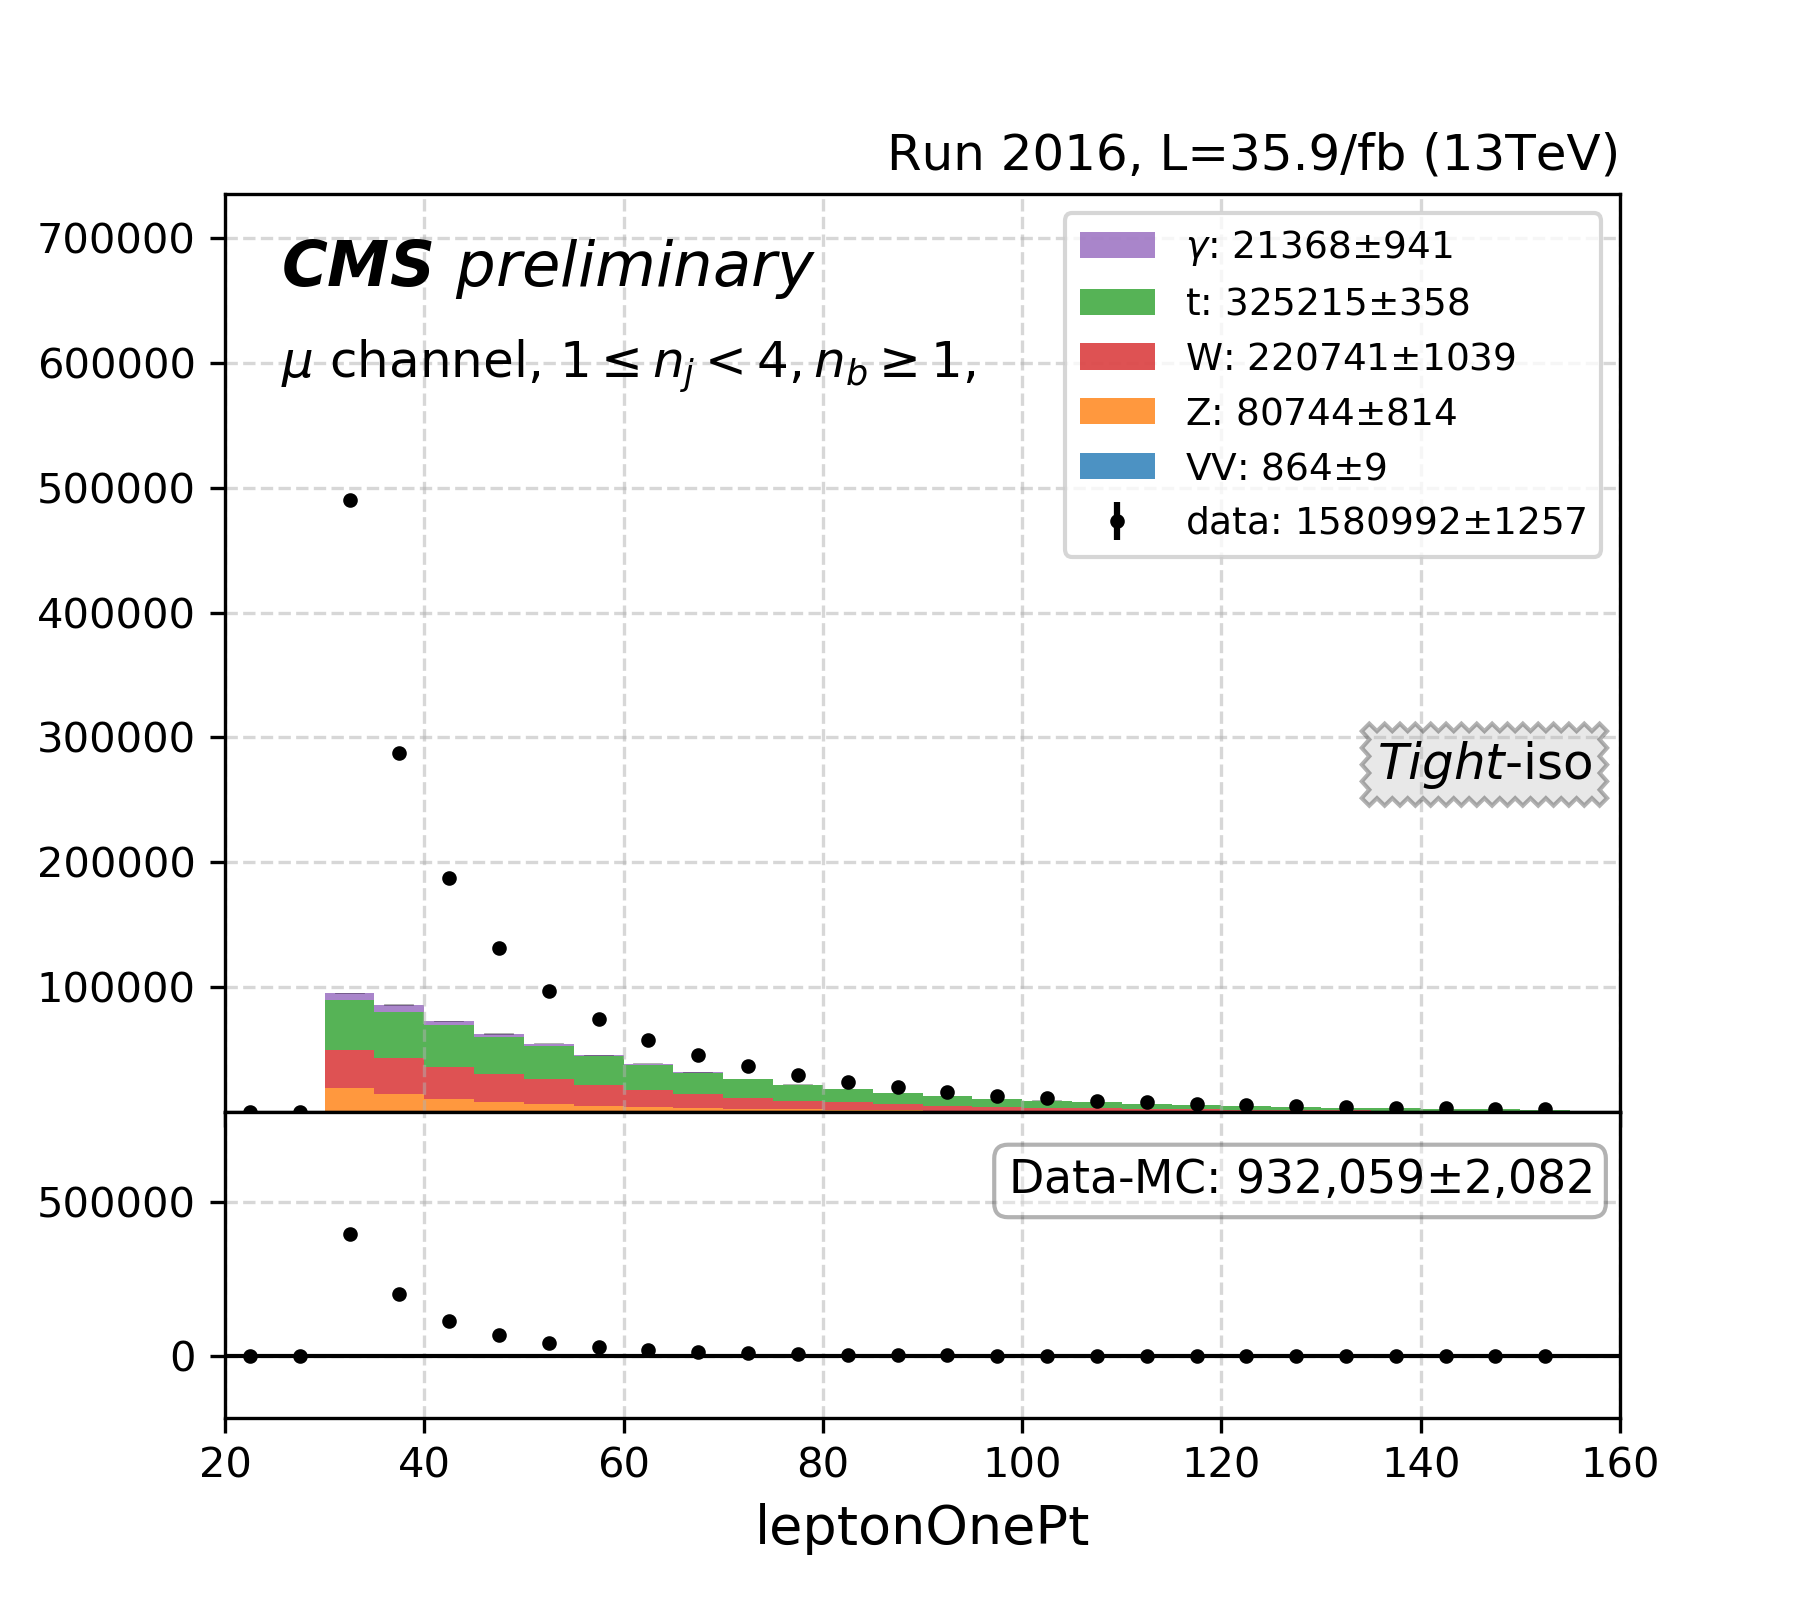
\includegraphics[width=0.24\textwidth]{chapters/Appendix/sectionQCD/figures/123j1b/mu_leptonOnePt_True.png}
    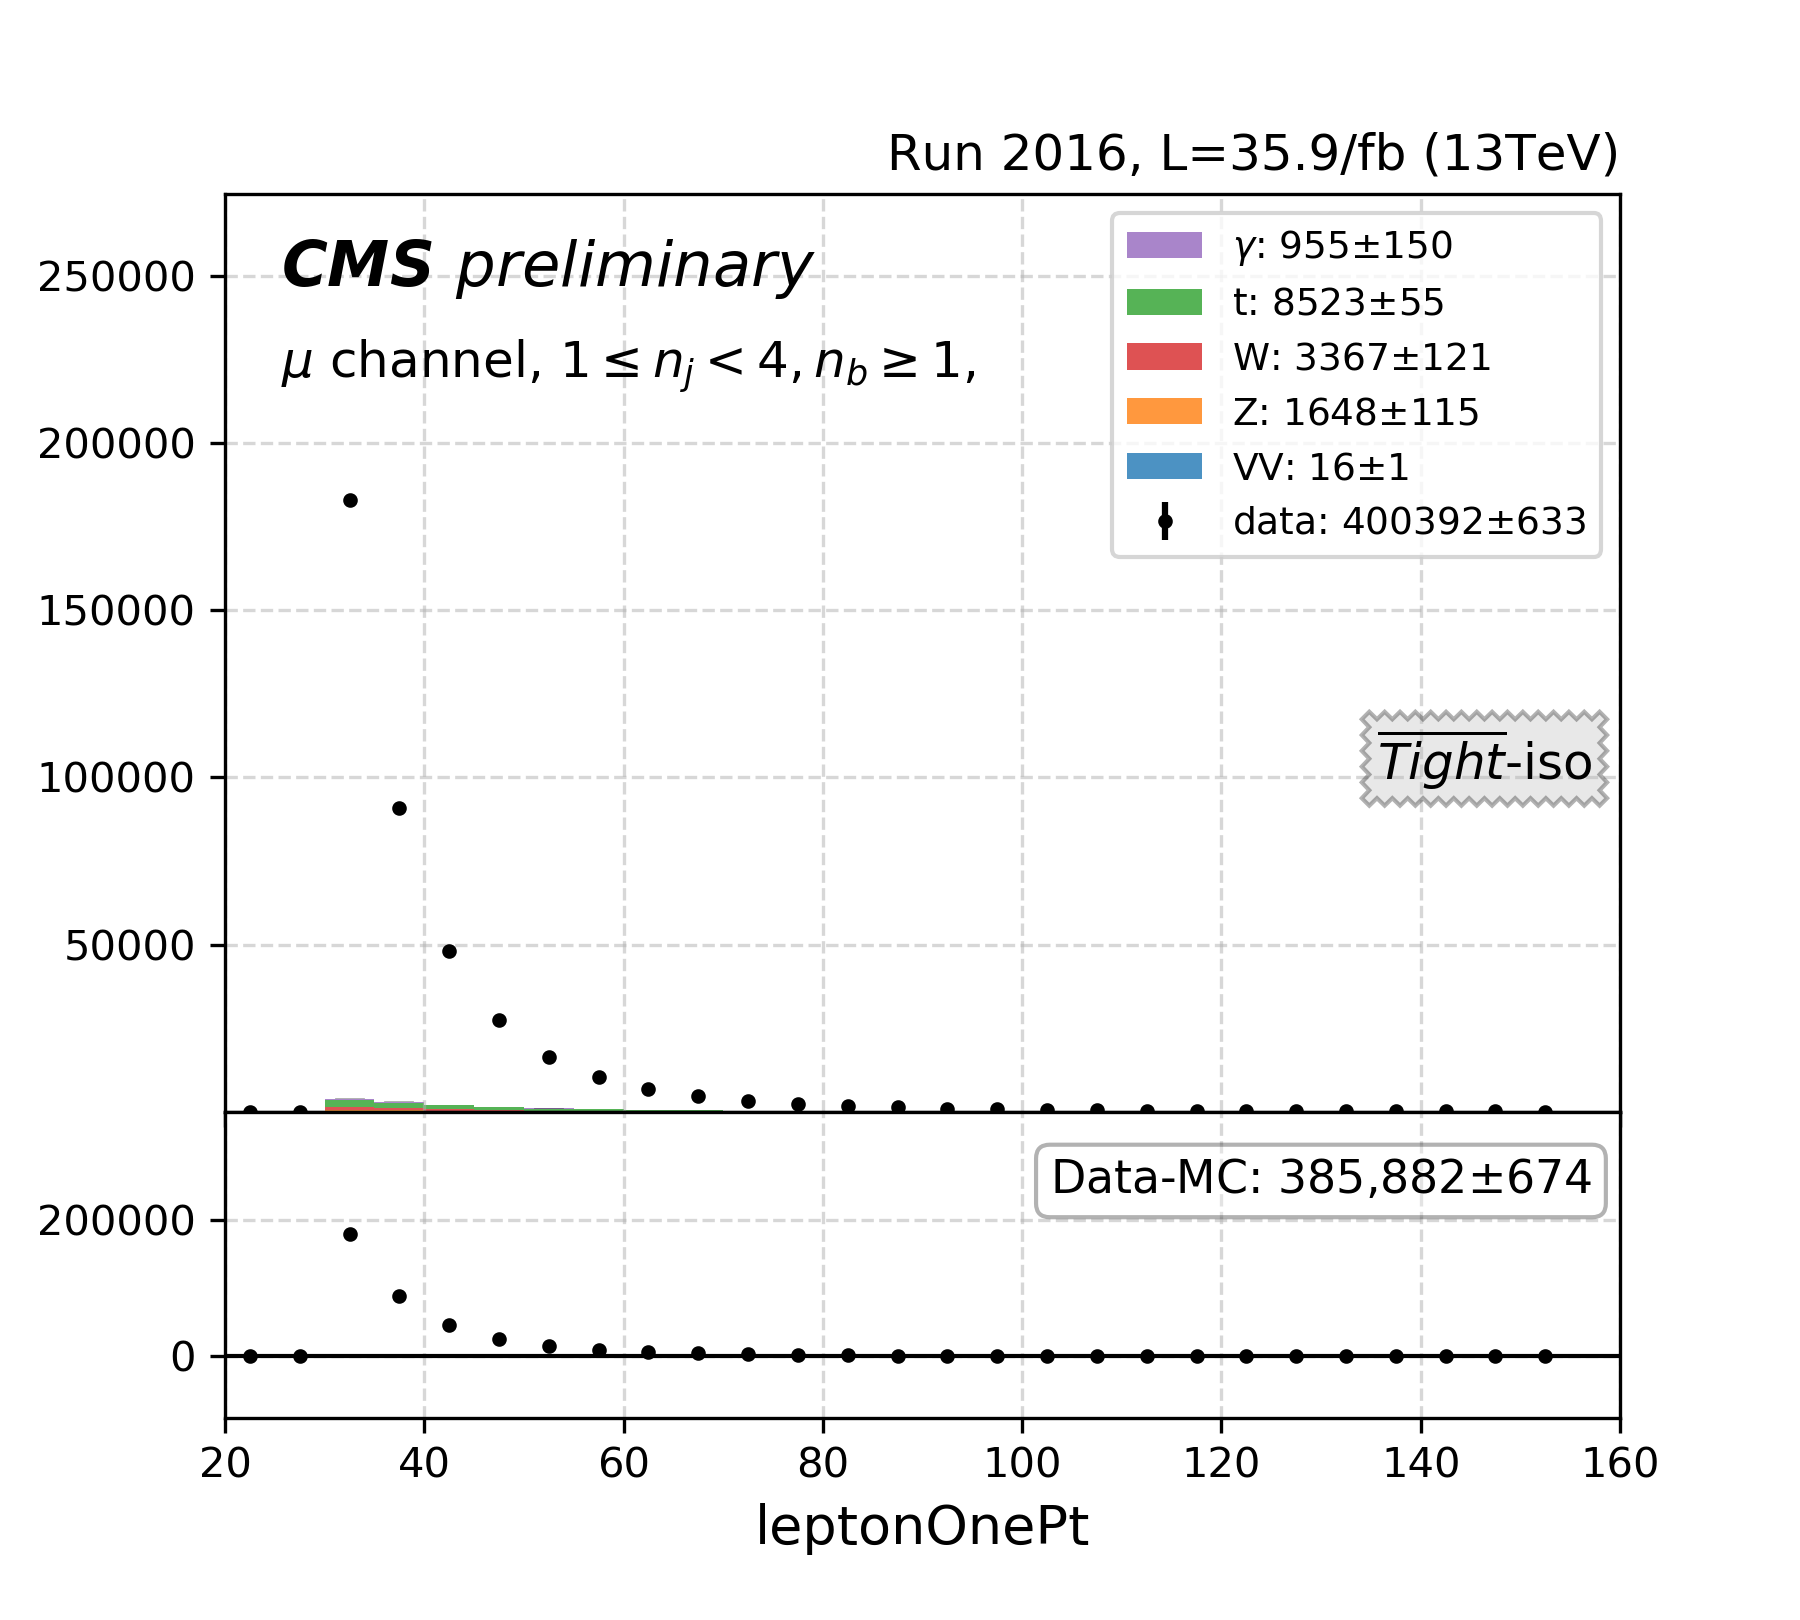
\includegraphics[width=0.24\textwidth]{chapters/Appendix/sectionQCD/figures/123j1b/mu_leptonOnePt_False.png}
    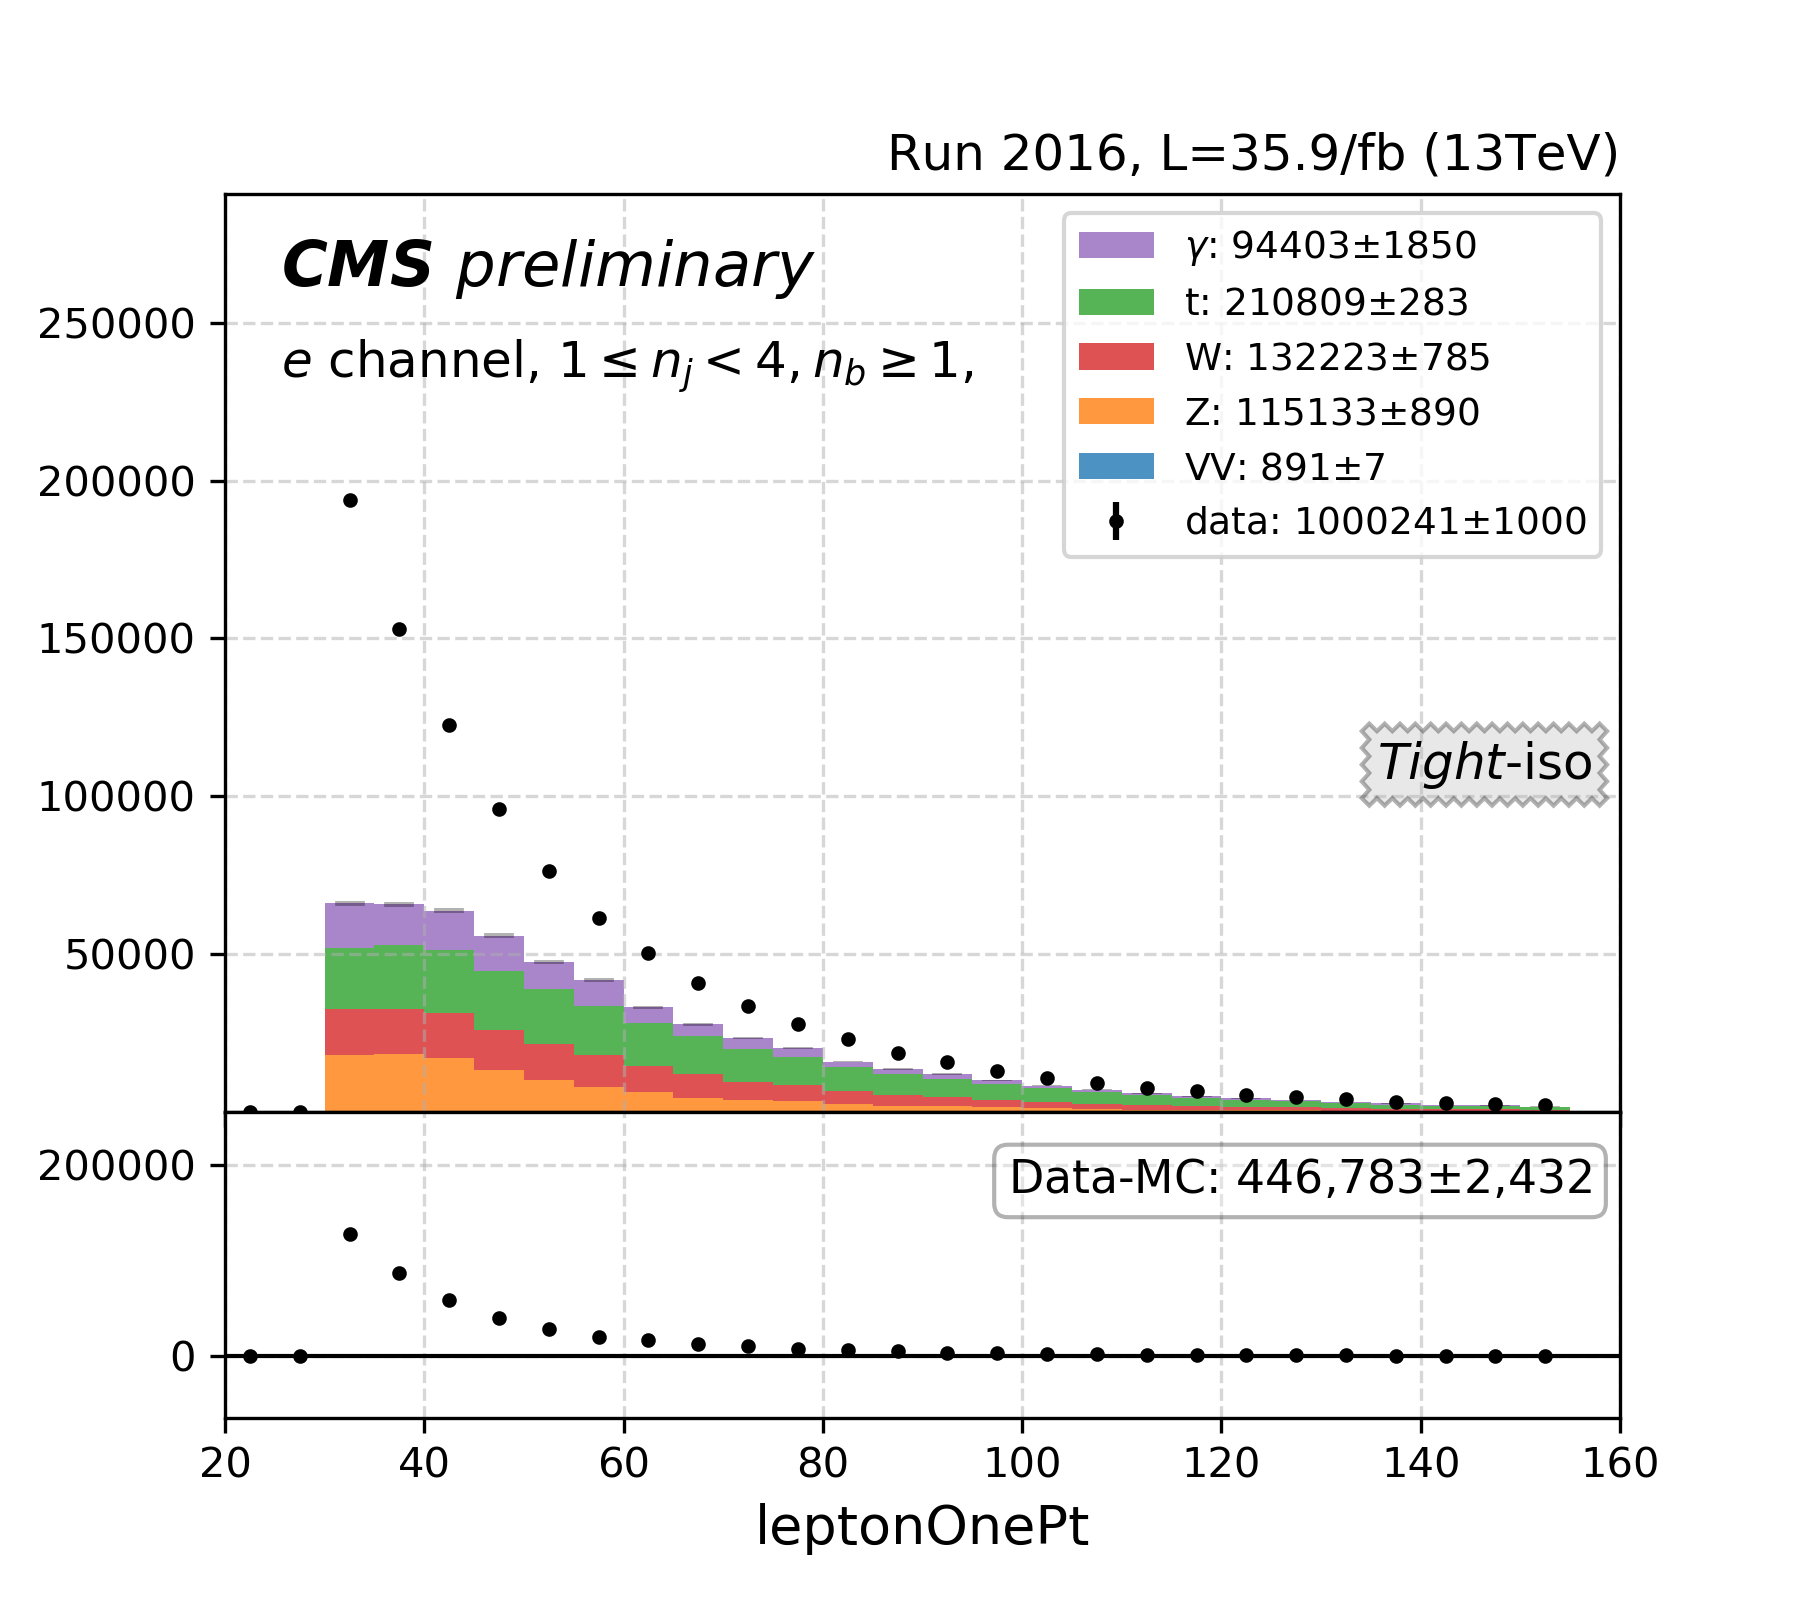
\includegraphics[width=0.24\textwidth]{chapters/Appendix/sectionQCD/figures/123j1b/e_leptonOnePt_True.png}
    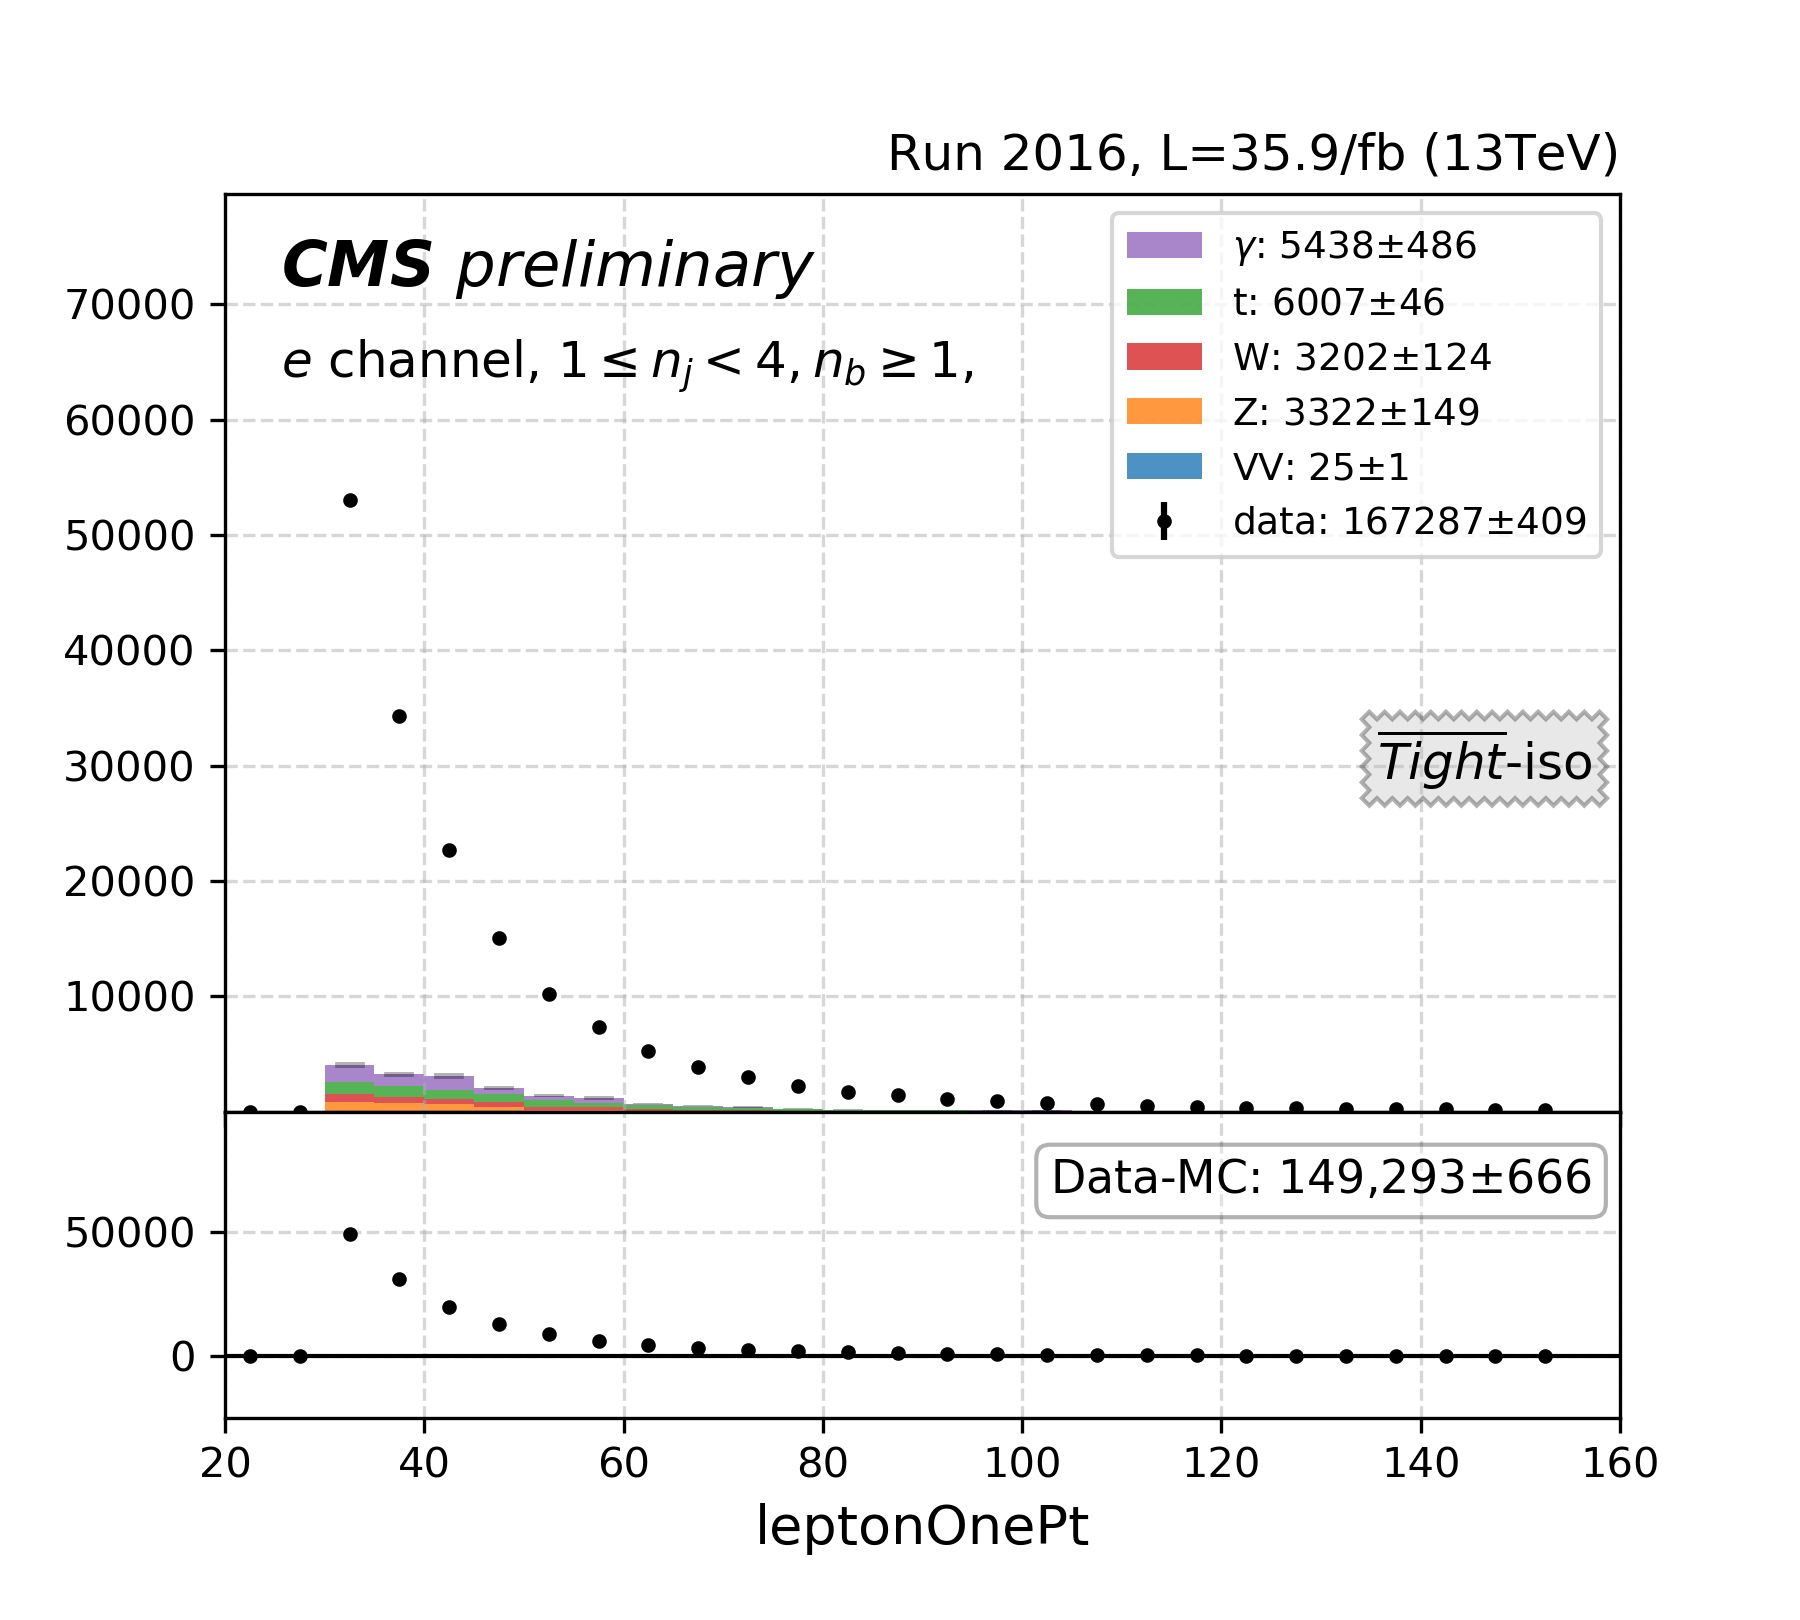
\includegraphics[width=0.24\textwidth]{chapters/Appendix/sectionQCD/figures/123j1b/e_leptonOnePt_False.png}
    
    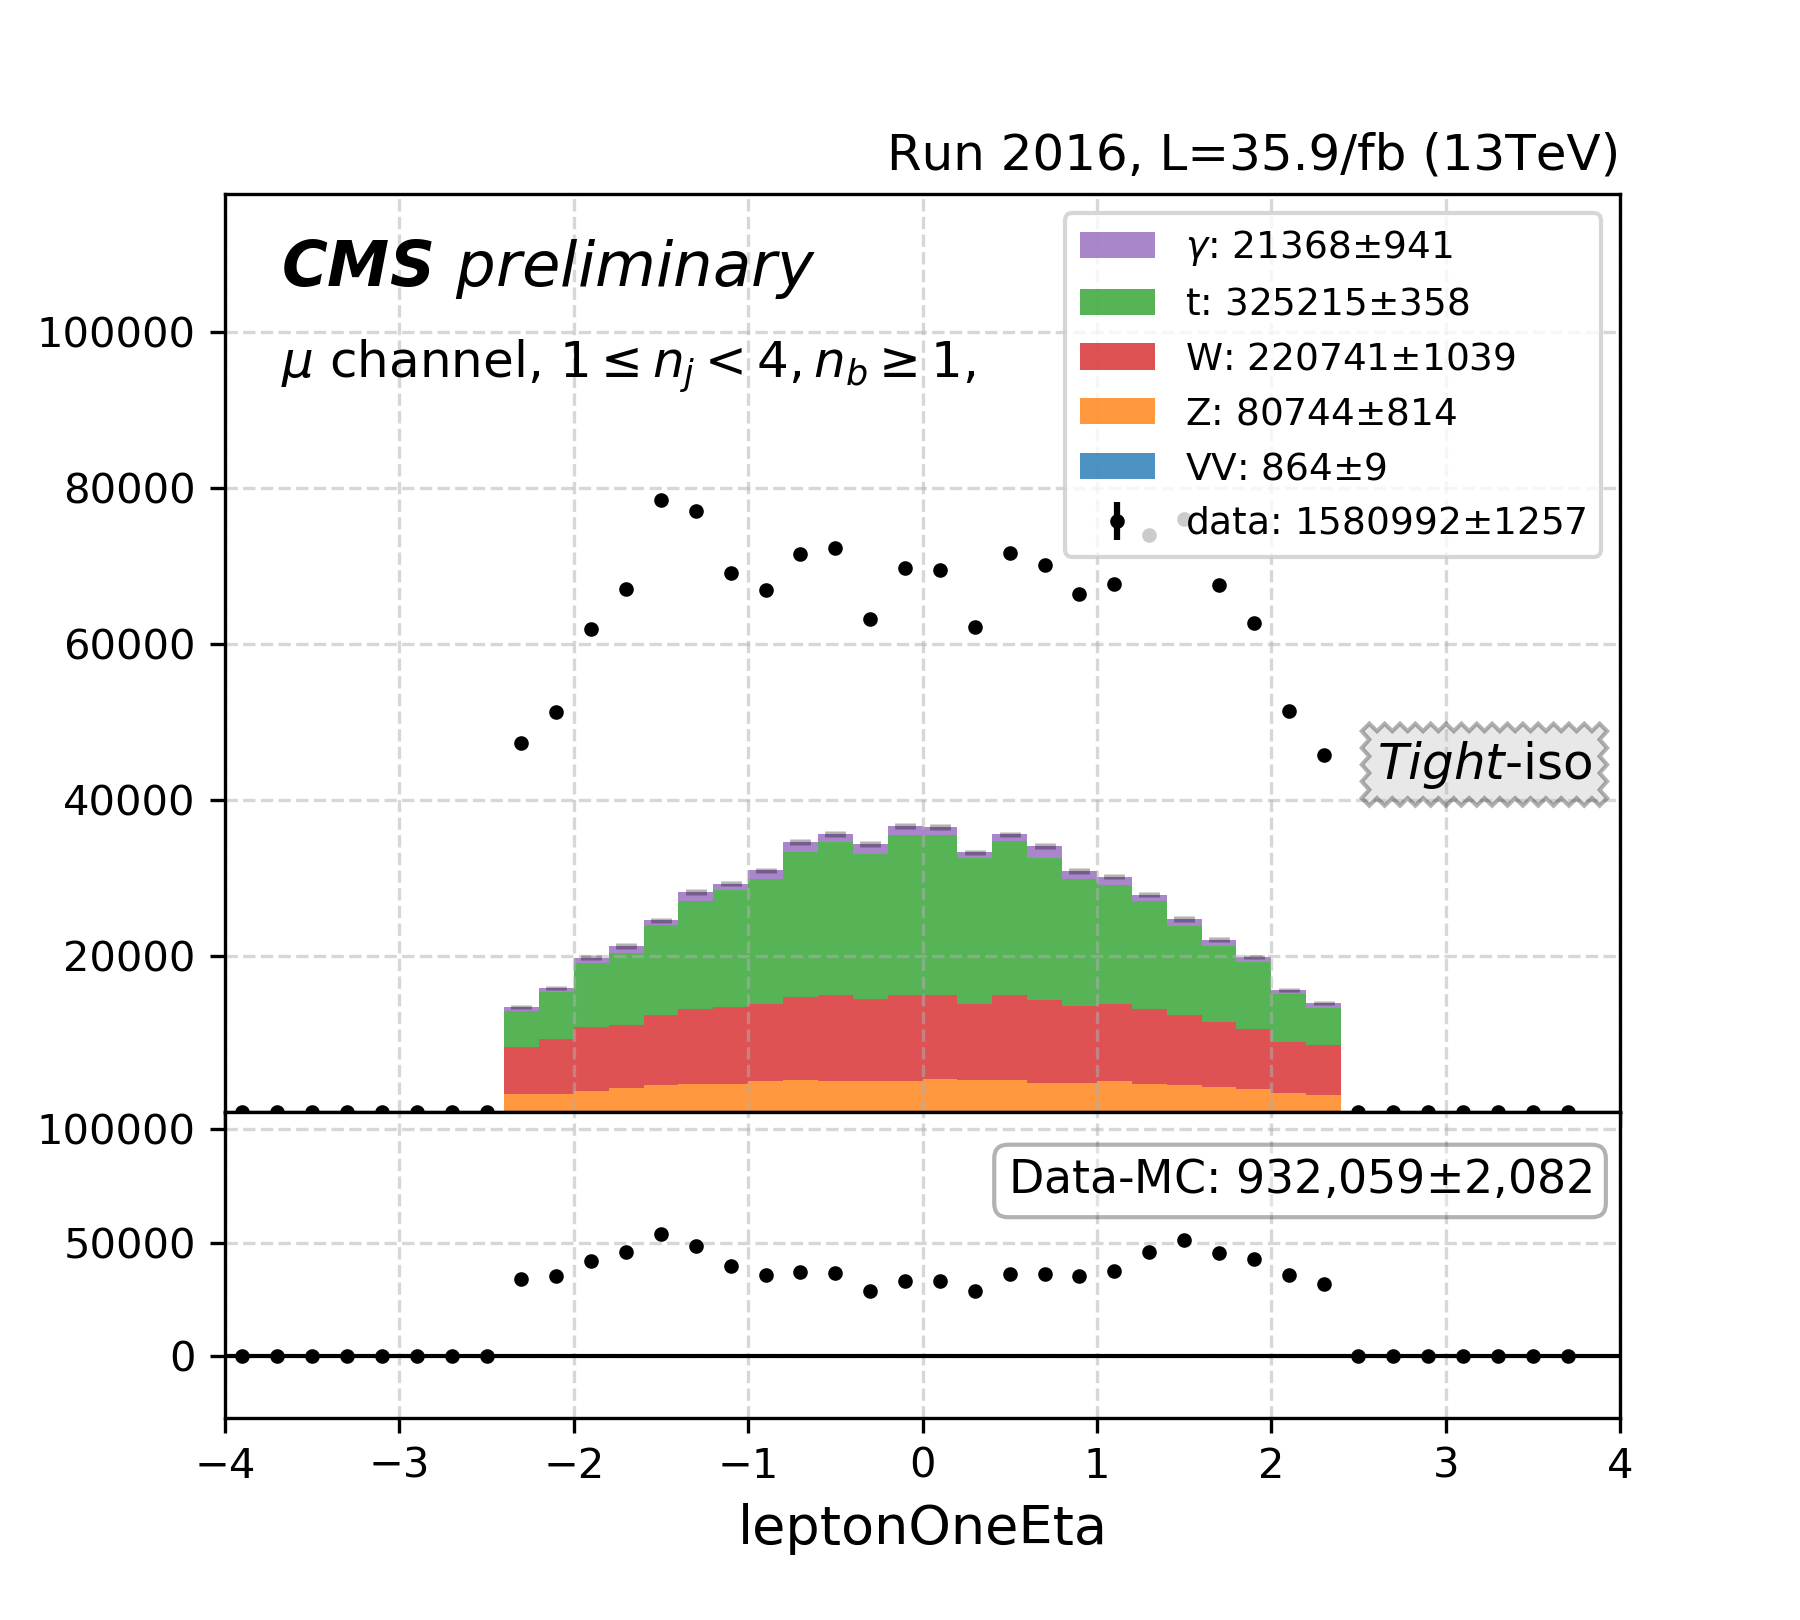
\includegraphics[width=0.24\textwidth]{chapters/Appendix/sectionQCD/figures/123j1b/mu_leptonOneEta_True.png}
    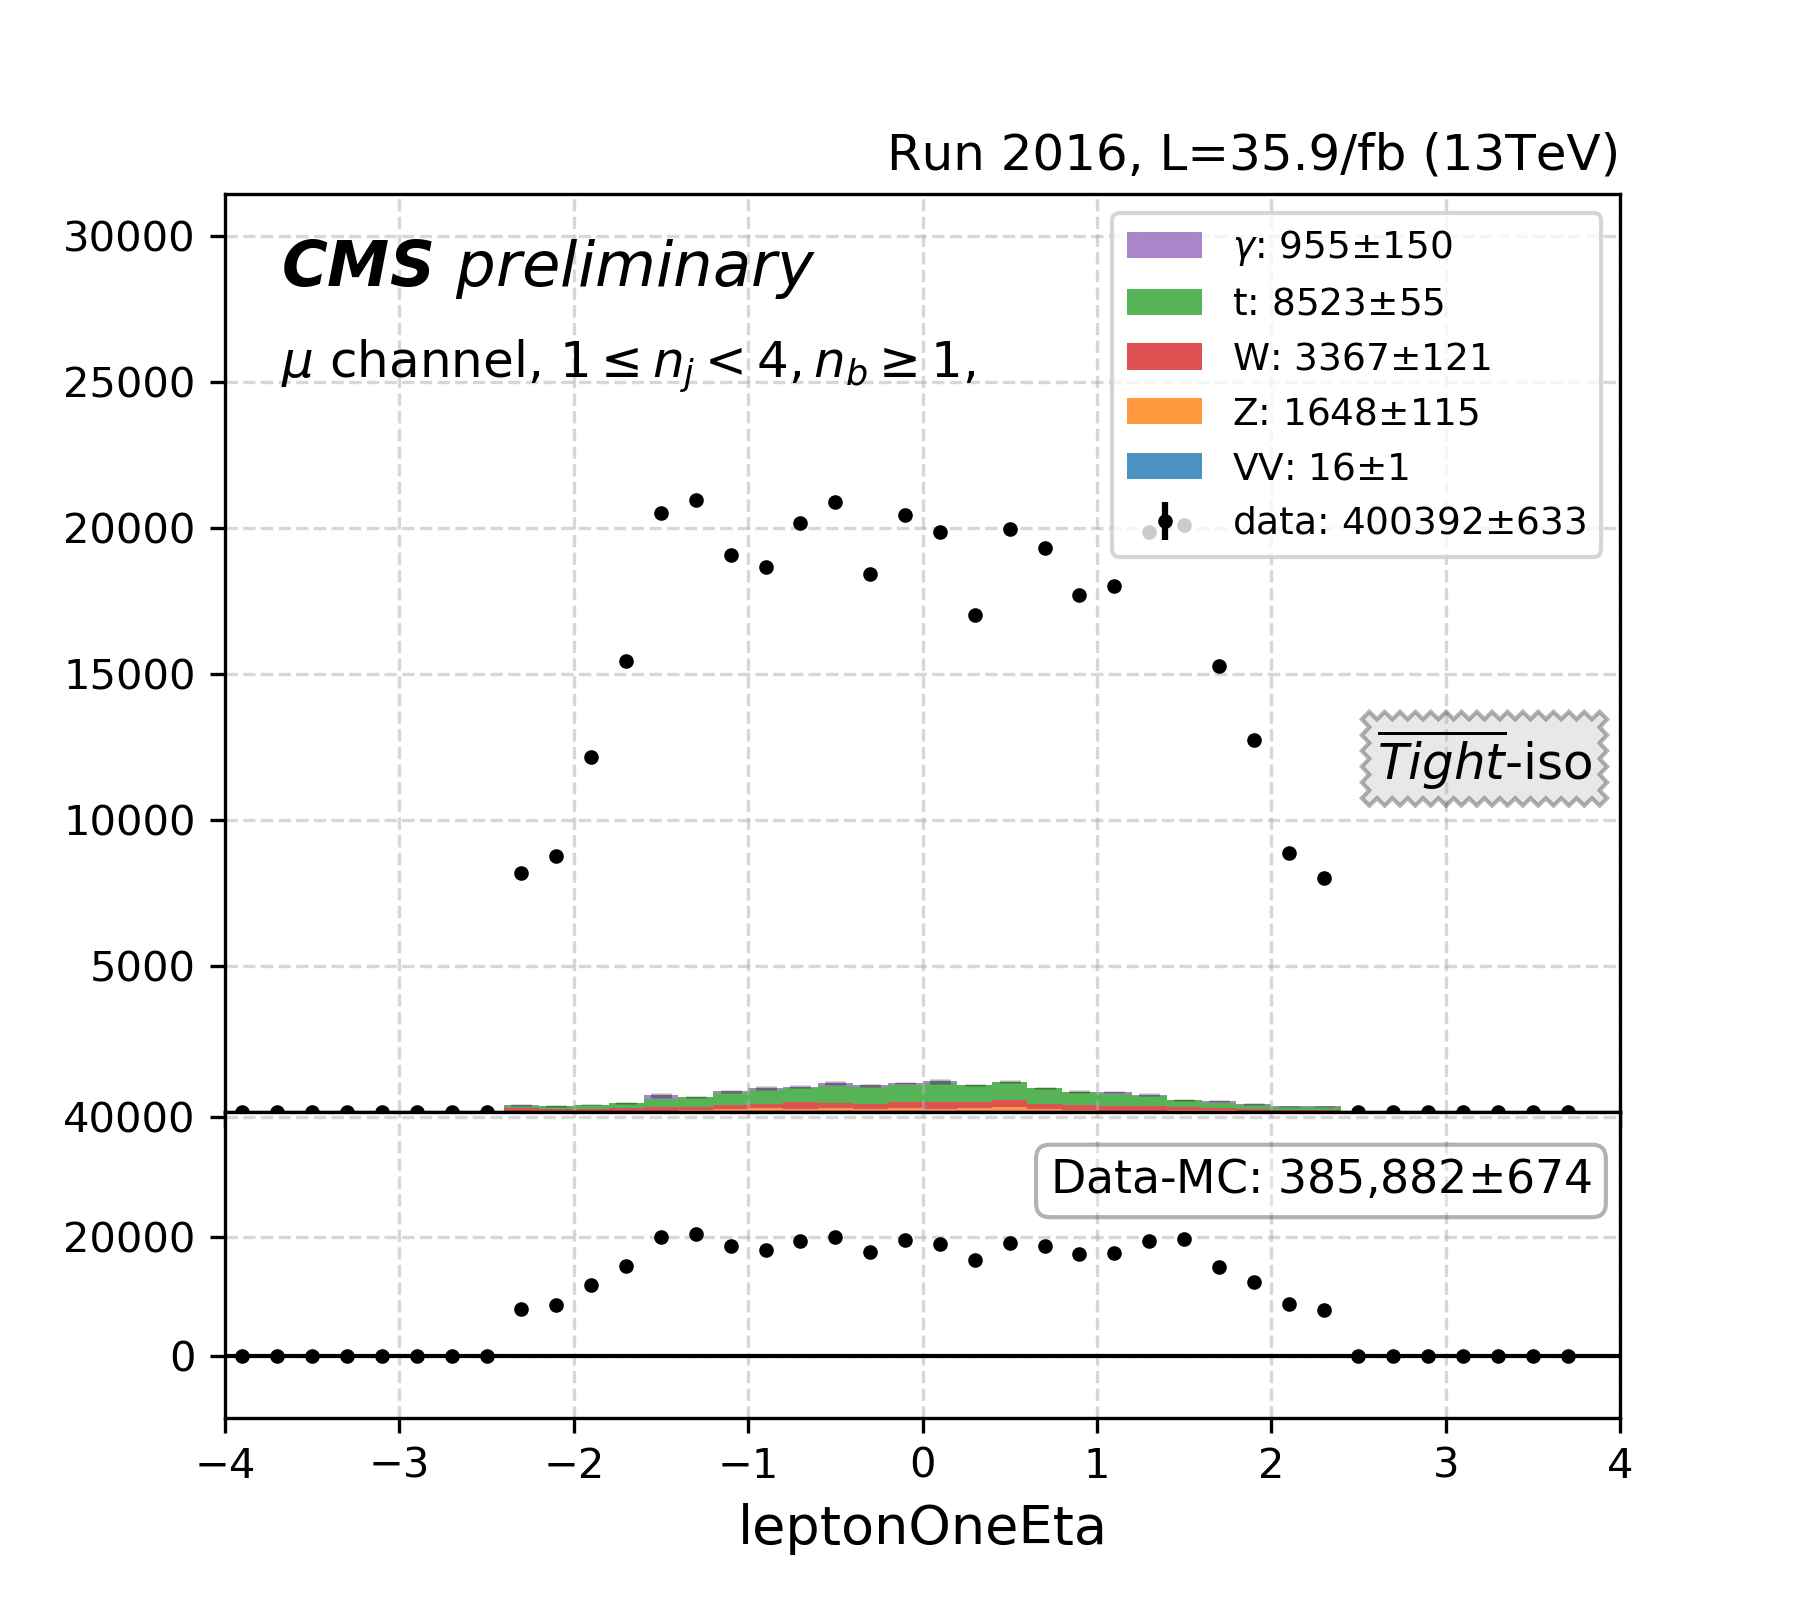
\includegraphics[width=0.24\textwidth]{chapters/Appendix/sectionQCD/figures/123j1b/mu_leptonOneEta_False.png}
    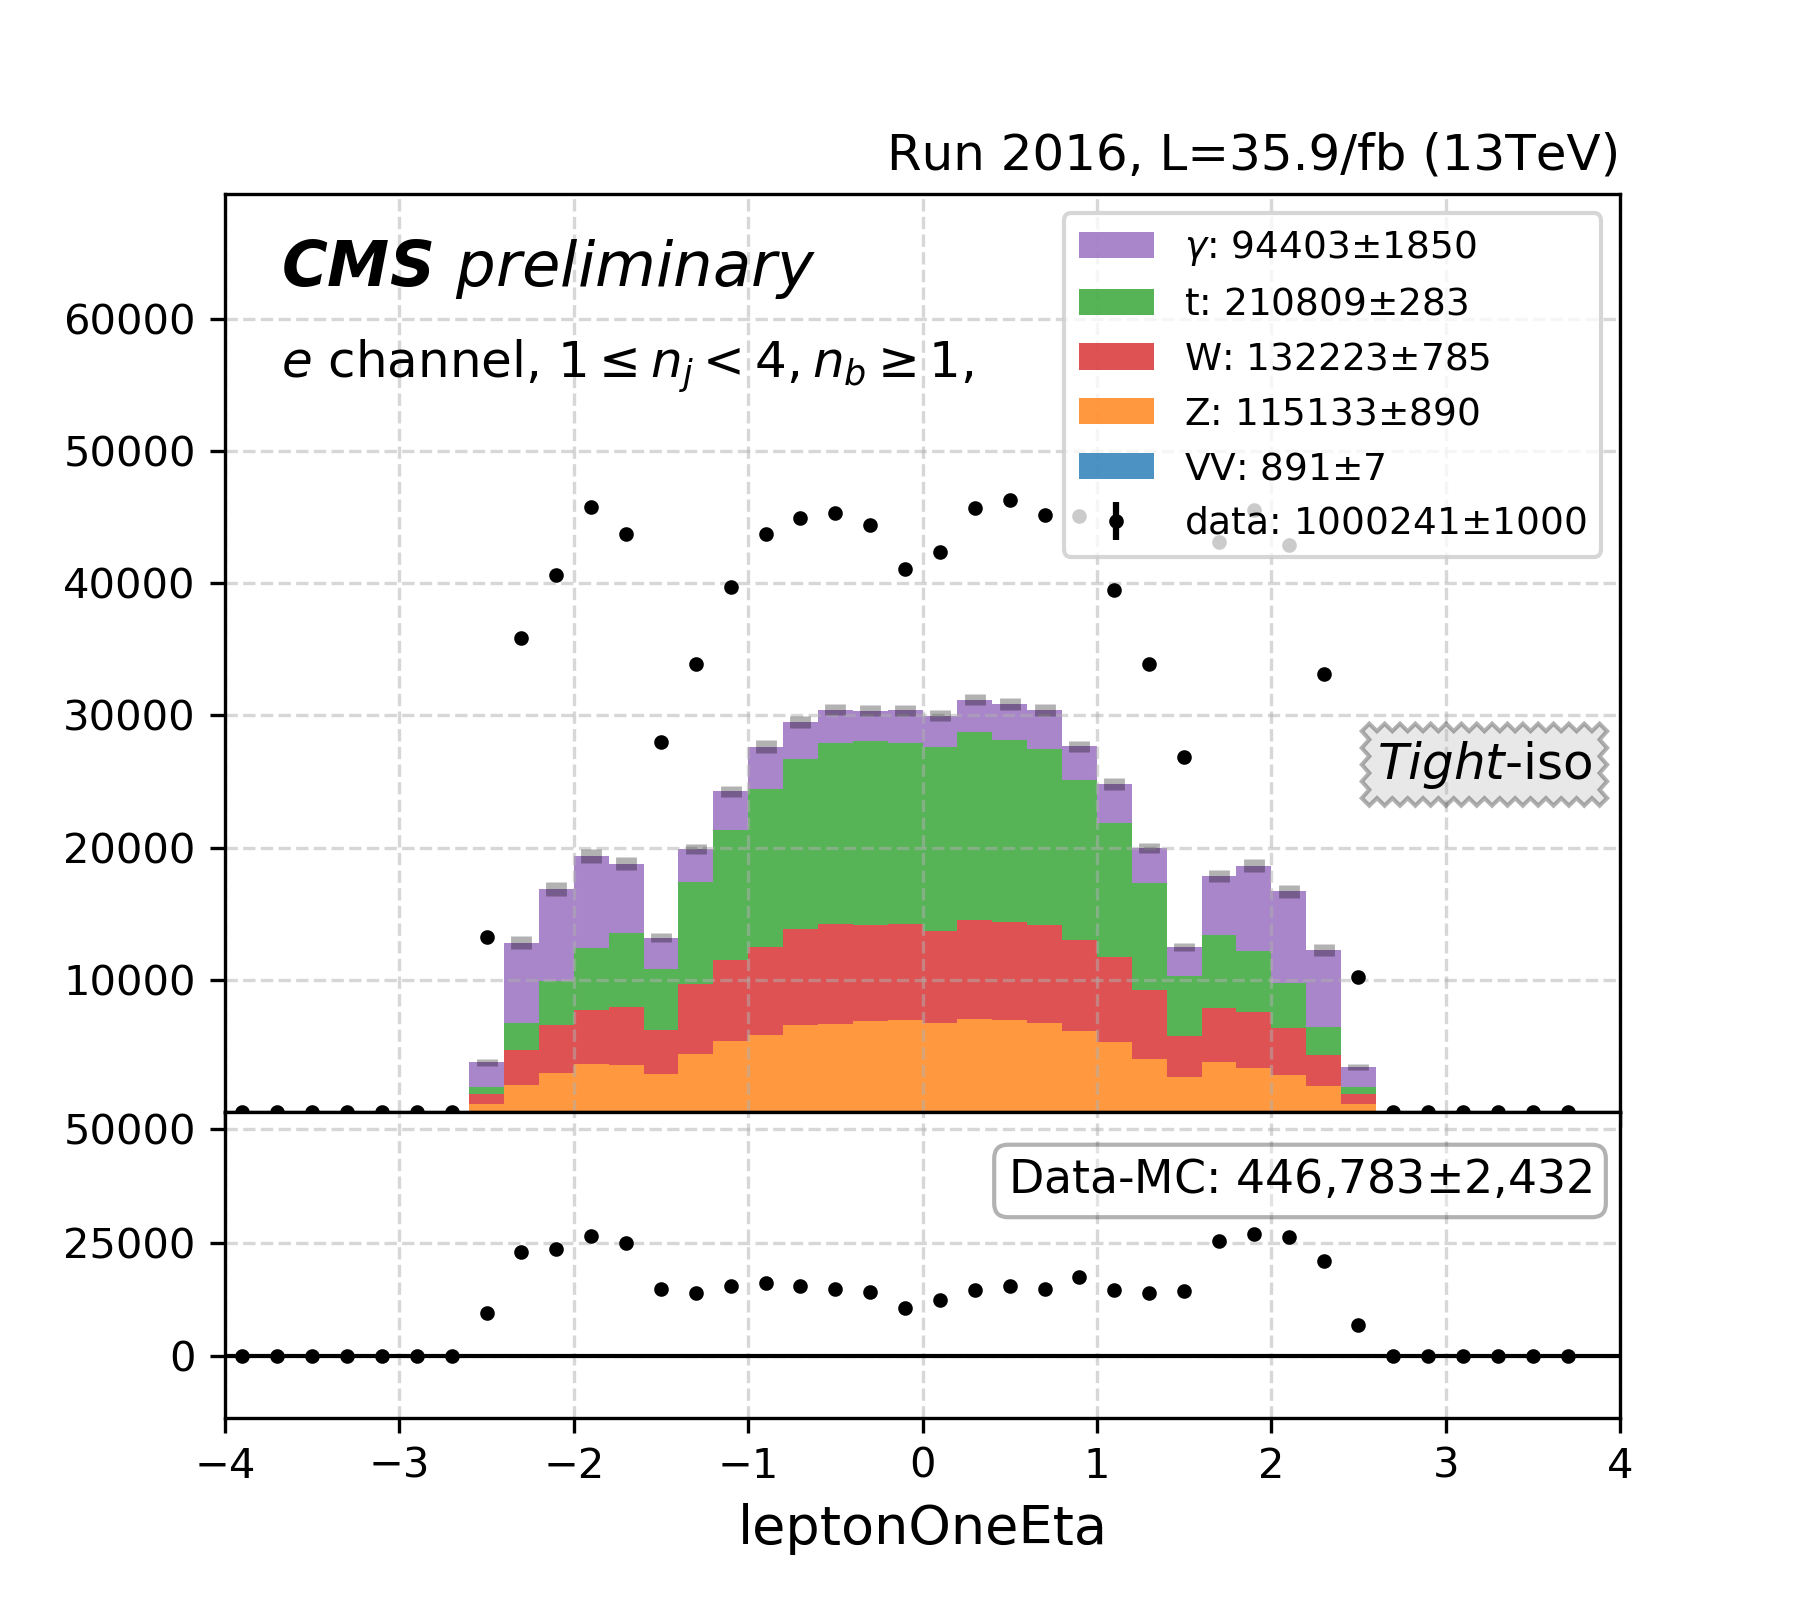
\includegraphics[width=0.24\textwidth]{chapters/Appendix/sectionQCD/figures/123j1b/e_leptonOneEta_True.png}
    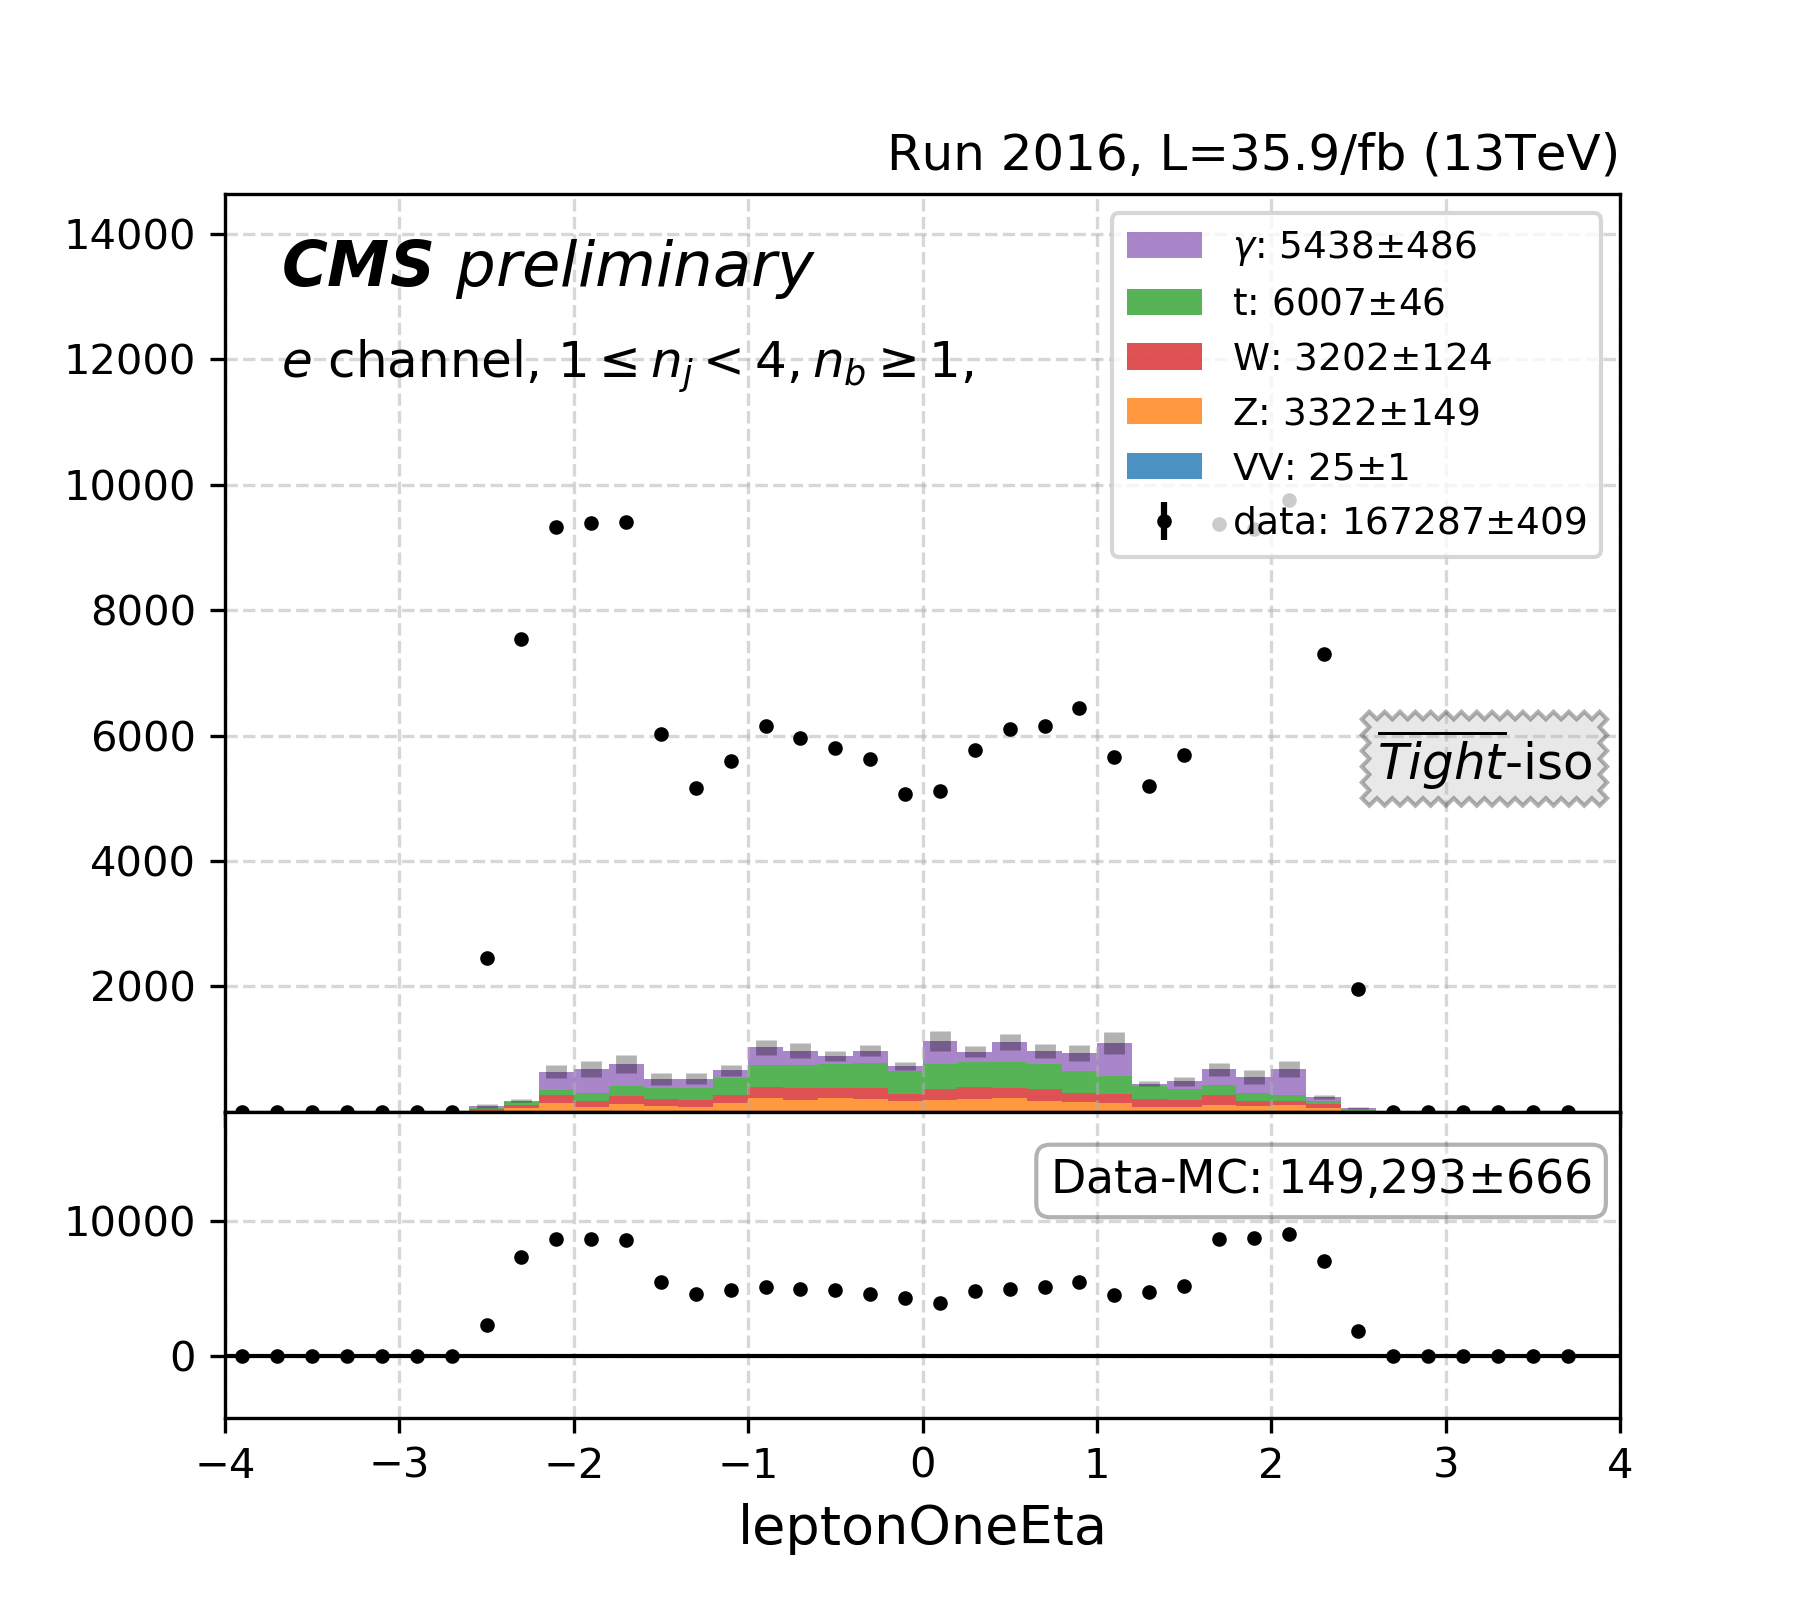
\includegraphics[width=0.24\textwidth]{chapters/Appendix/sectionQCD/figures/123j1b/e_leptonOneEta_False.png}
    
    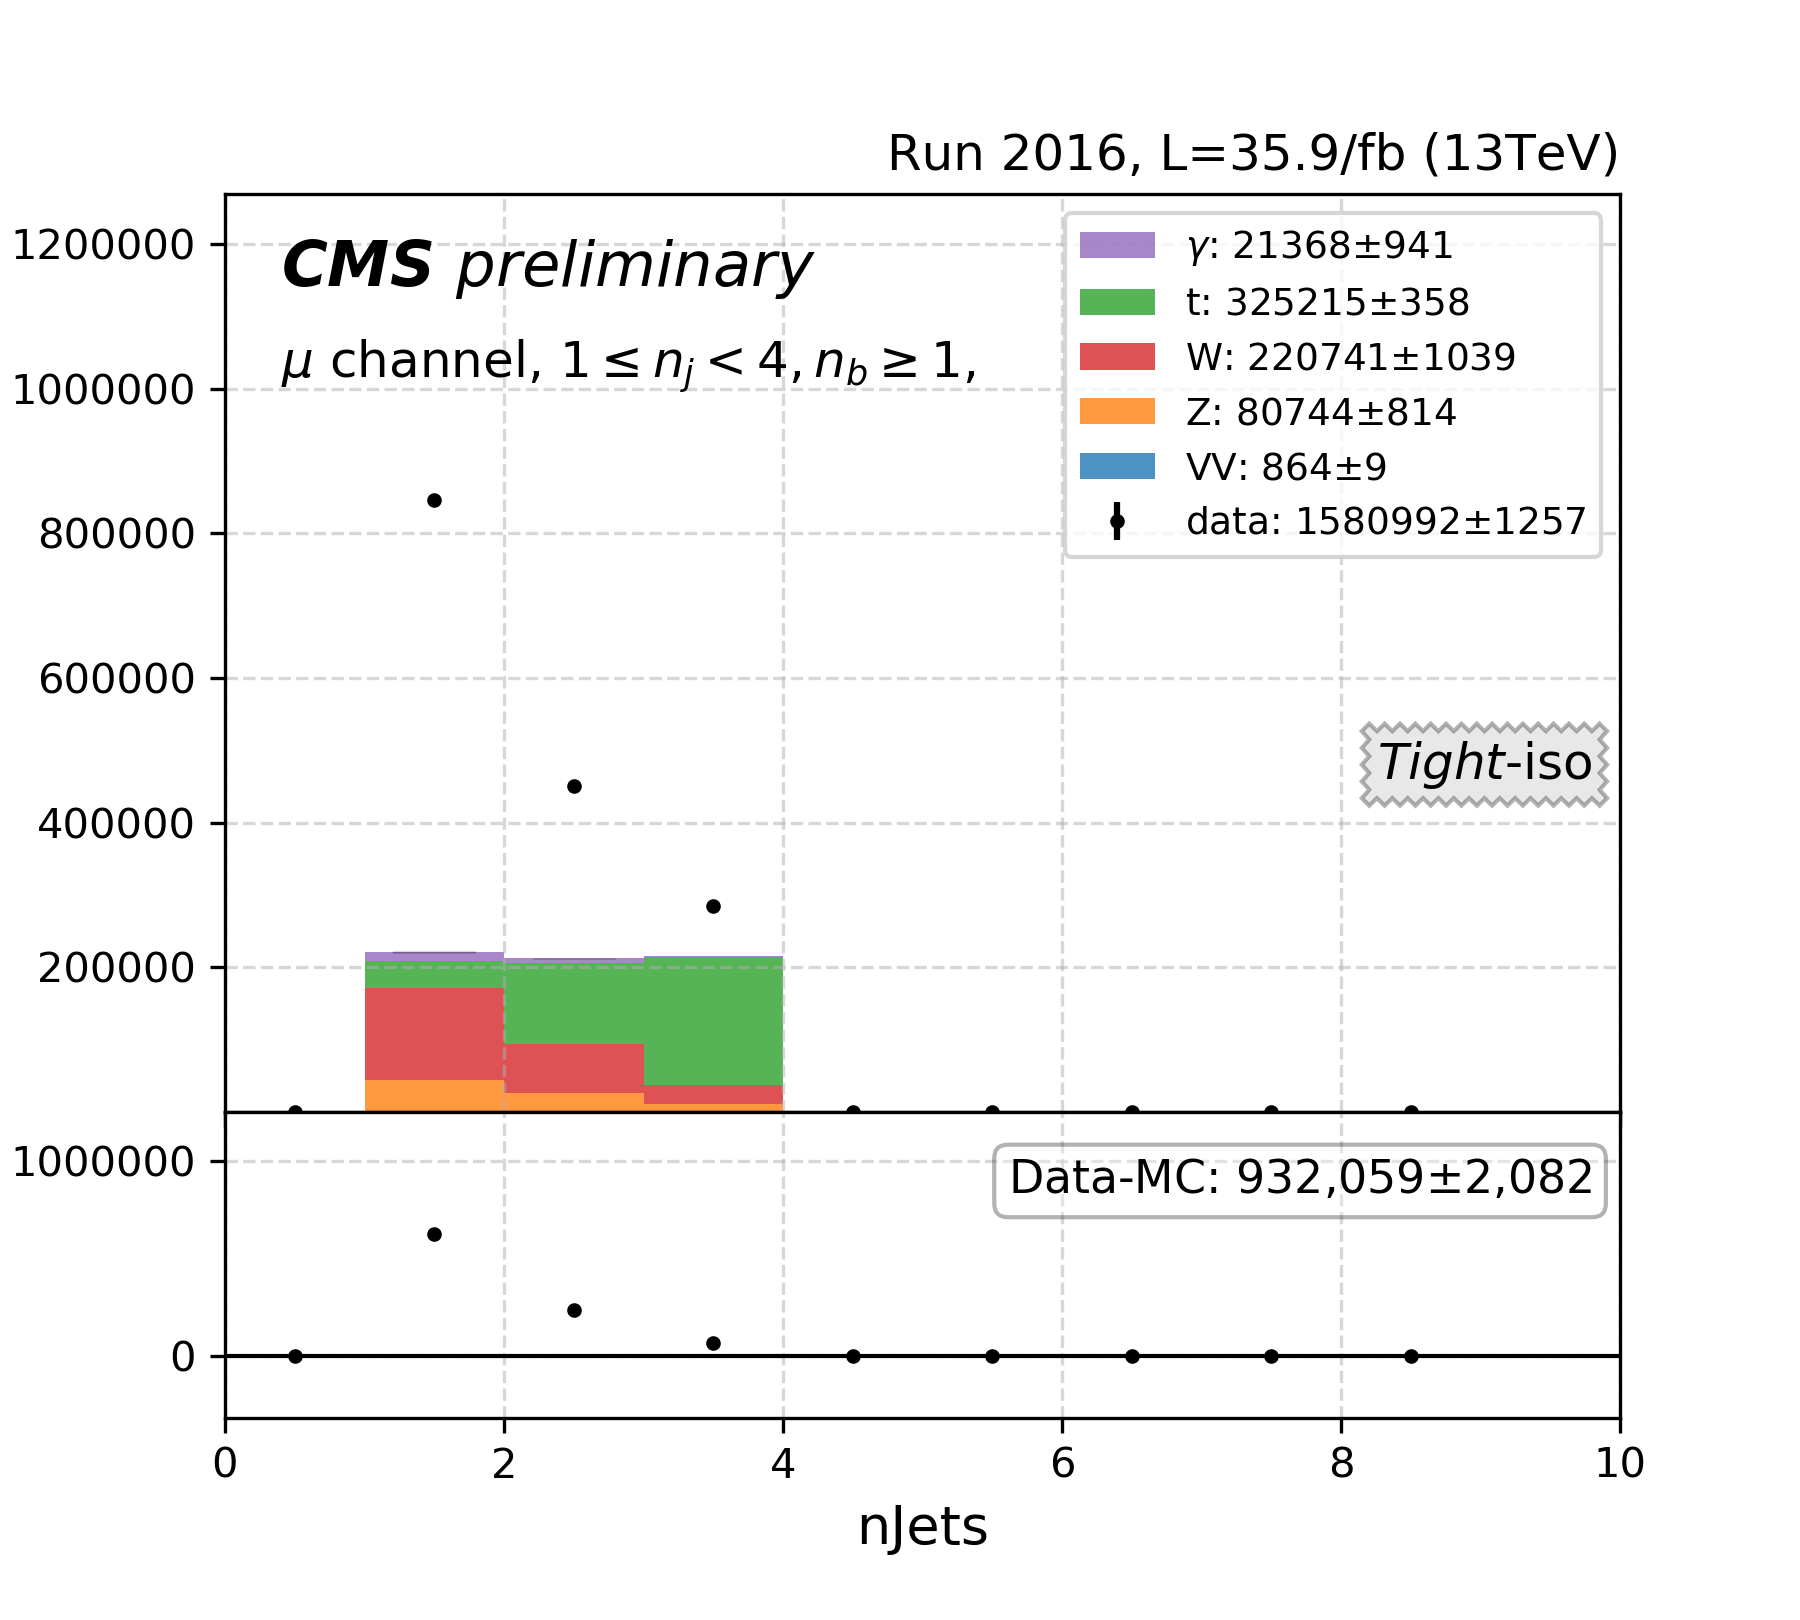
\includegraphics[width=0.24\textwidth]{chapters/Appendix/sectionQCD/figures/123j1b/mu_nJets_True.png}
    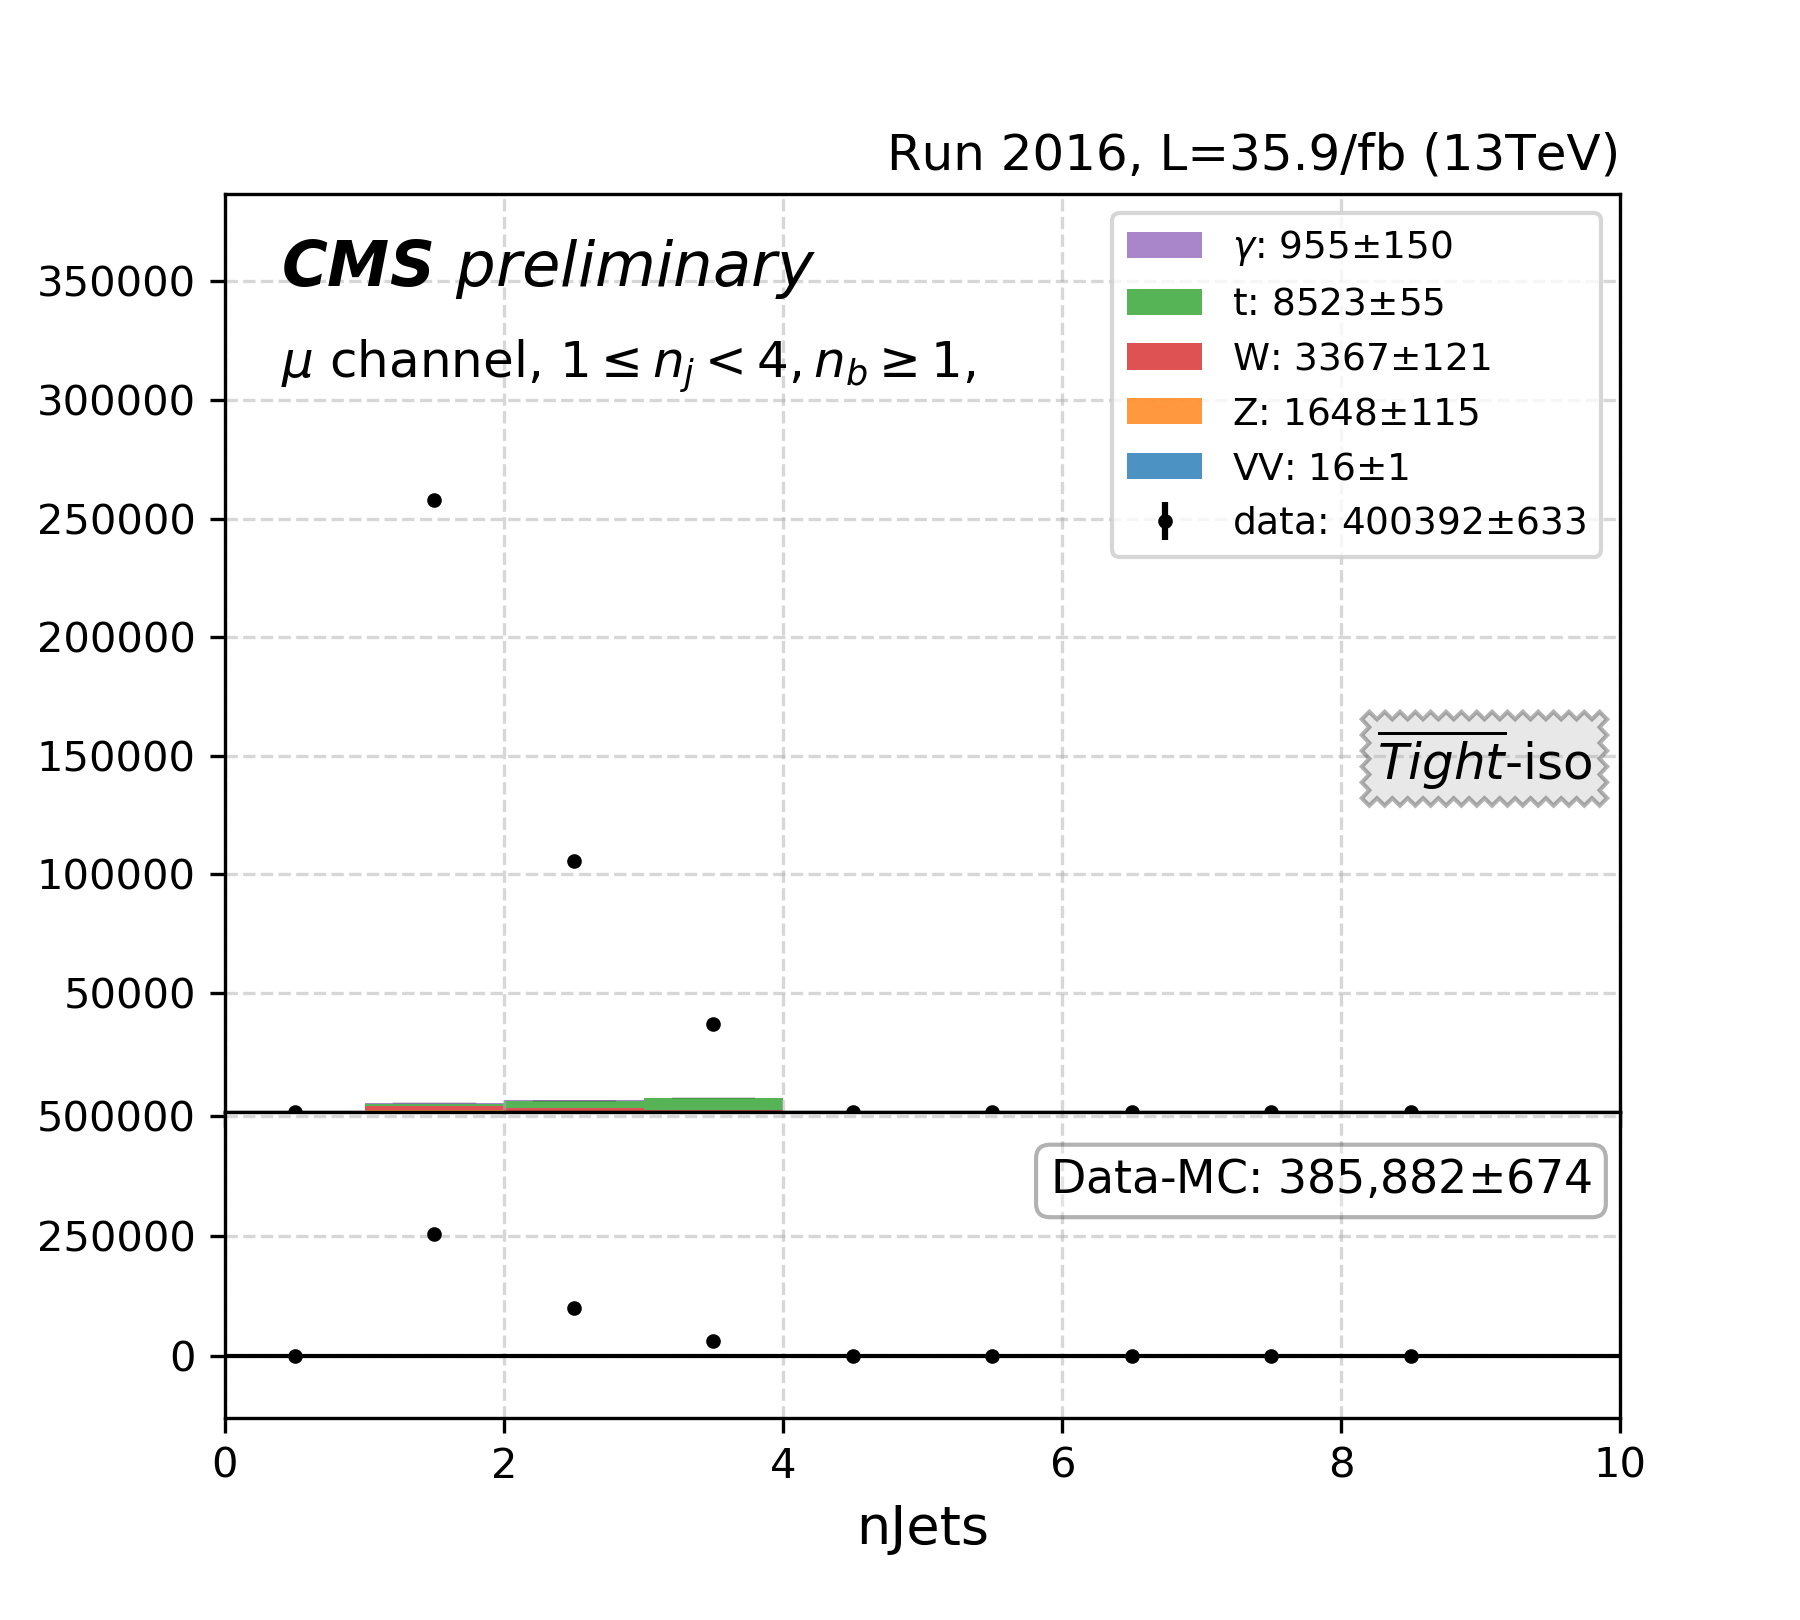
\includegraphics[width=0.24\textwidth]{chapters/Appendix/sectionQCD/figures/123j1b/mu_nJets_False.png}
    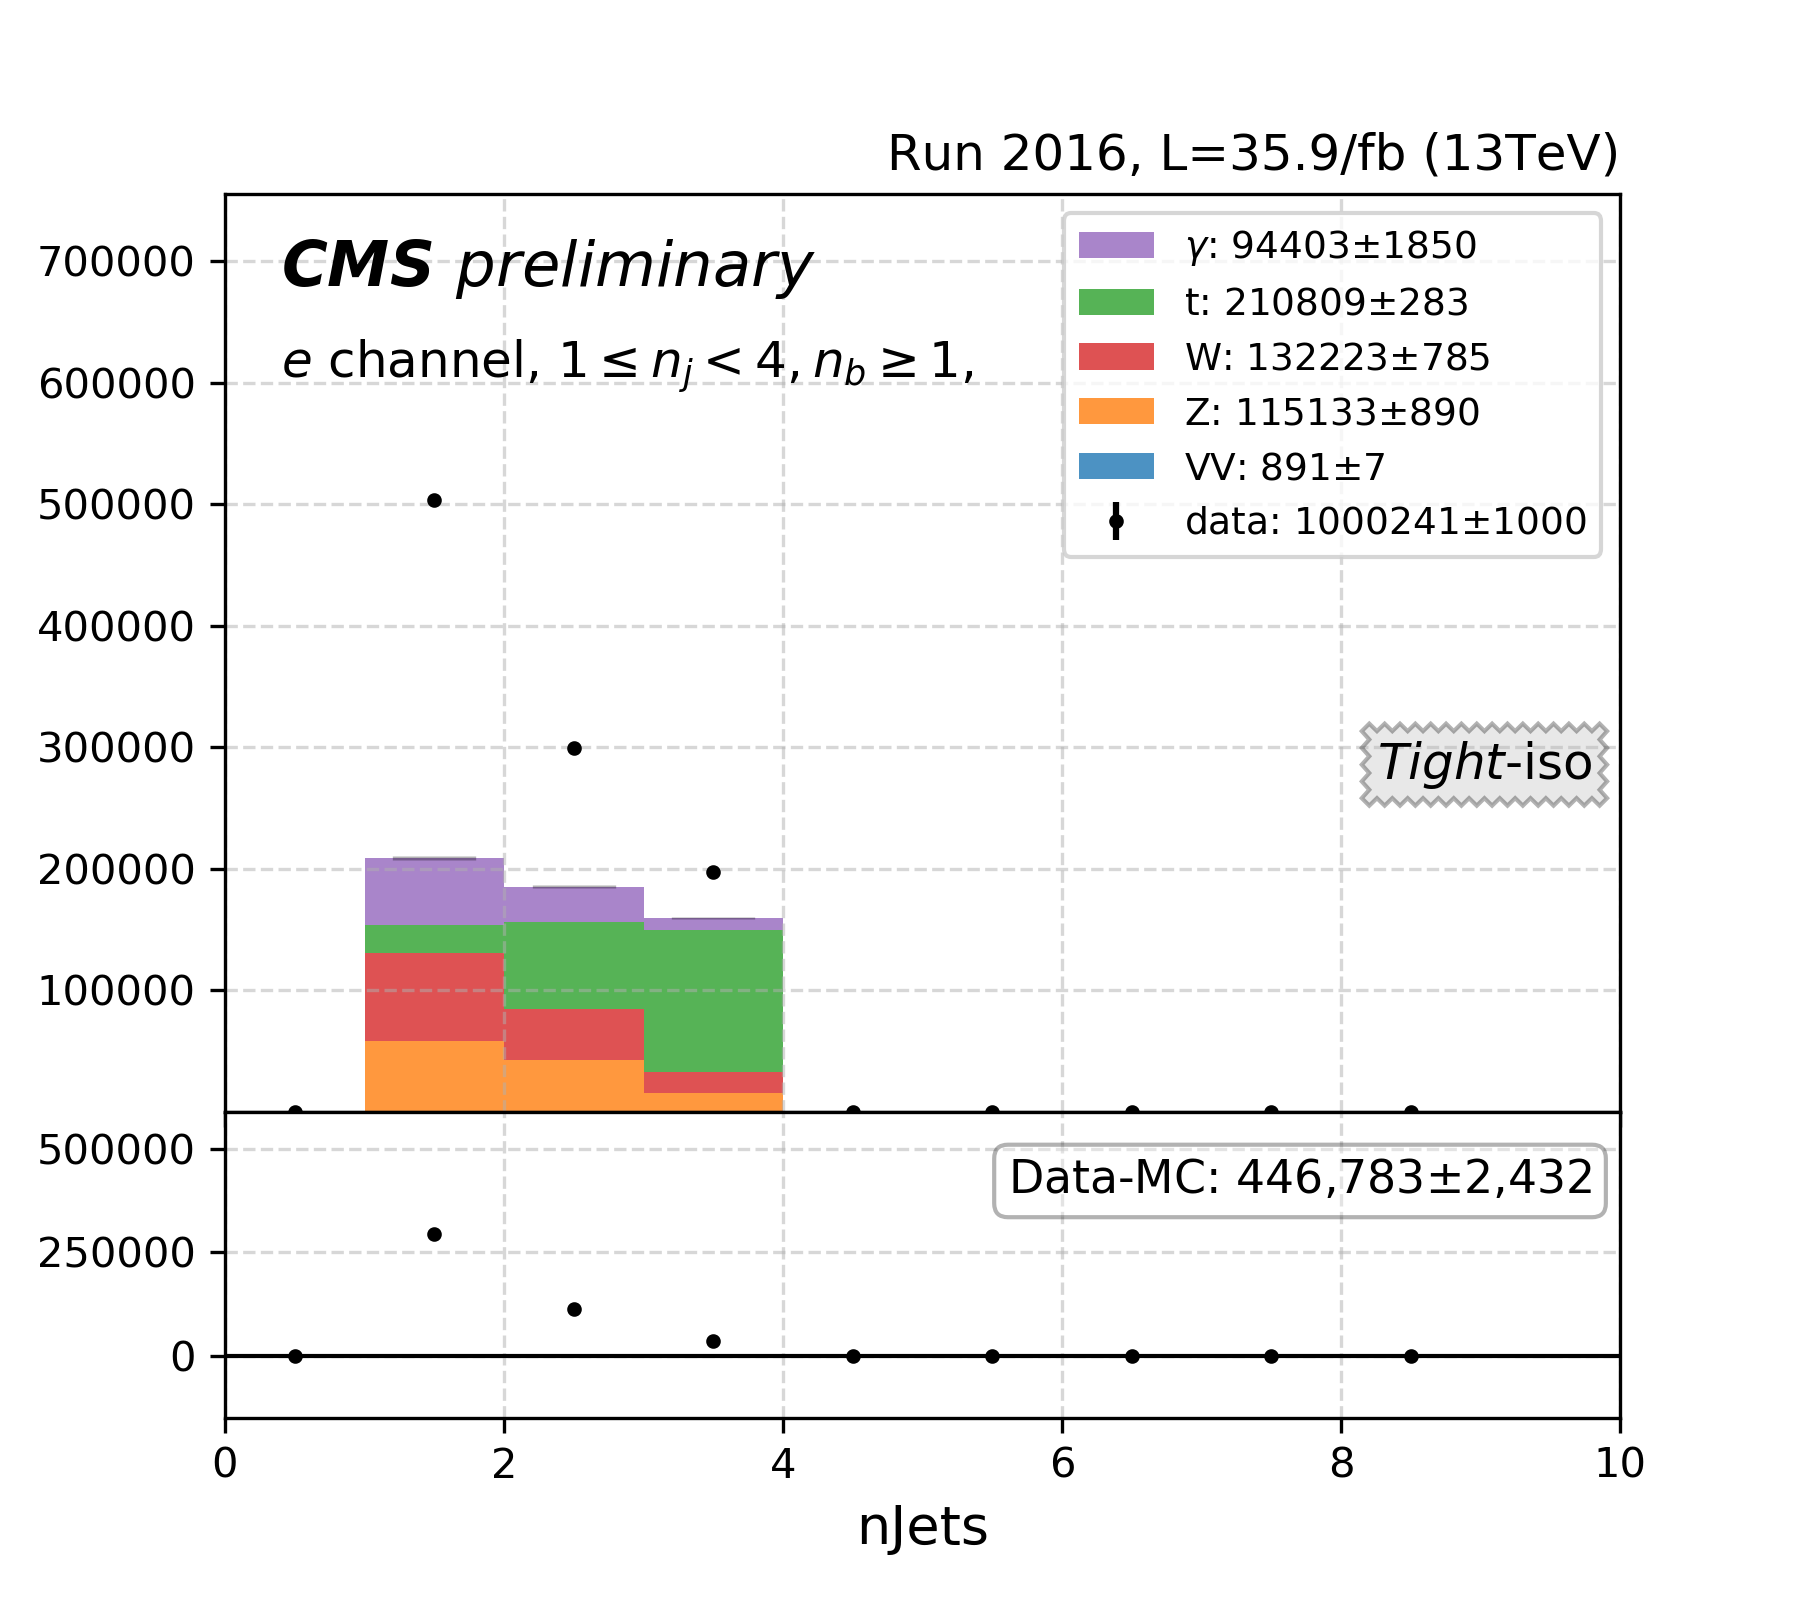
\includegraphics[width=0.24\textwidth]{chapters/Appendix/sectionQCD/figures/123j1b/e_nJets_True.png}
    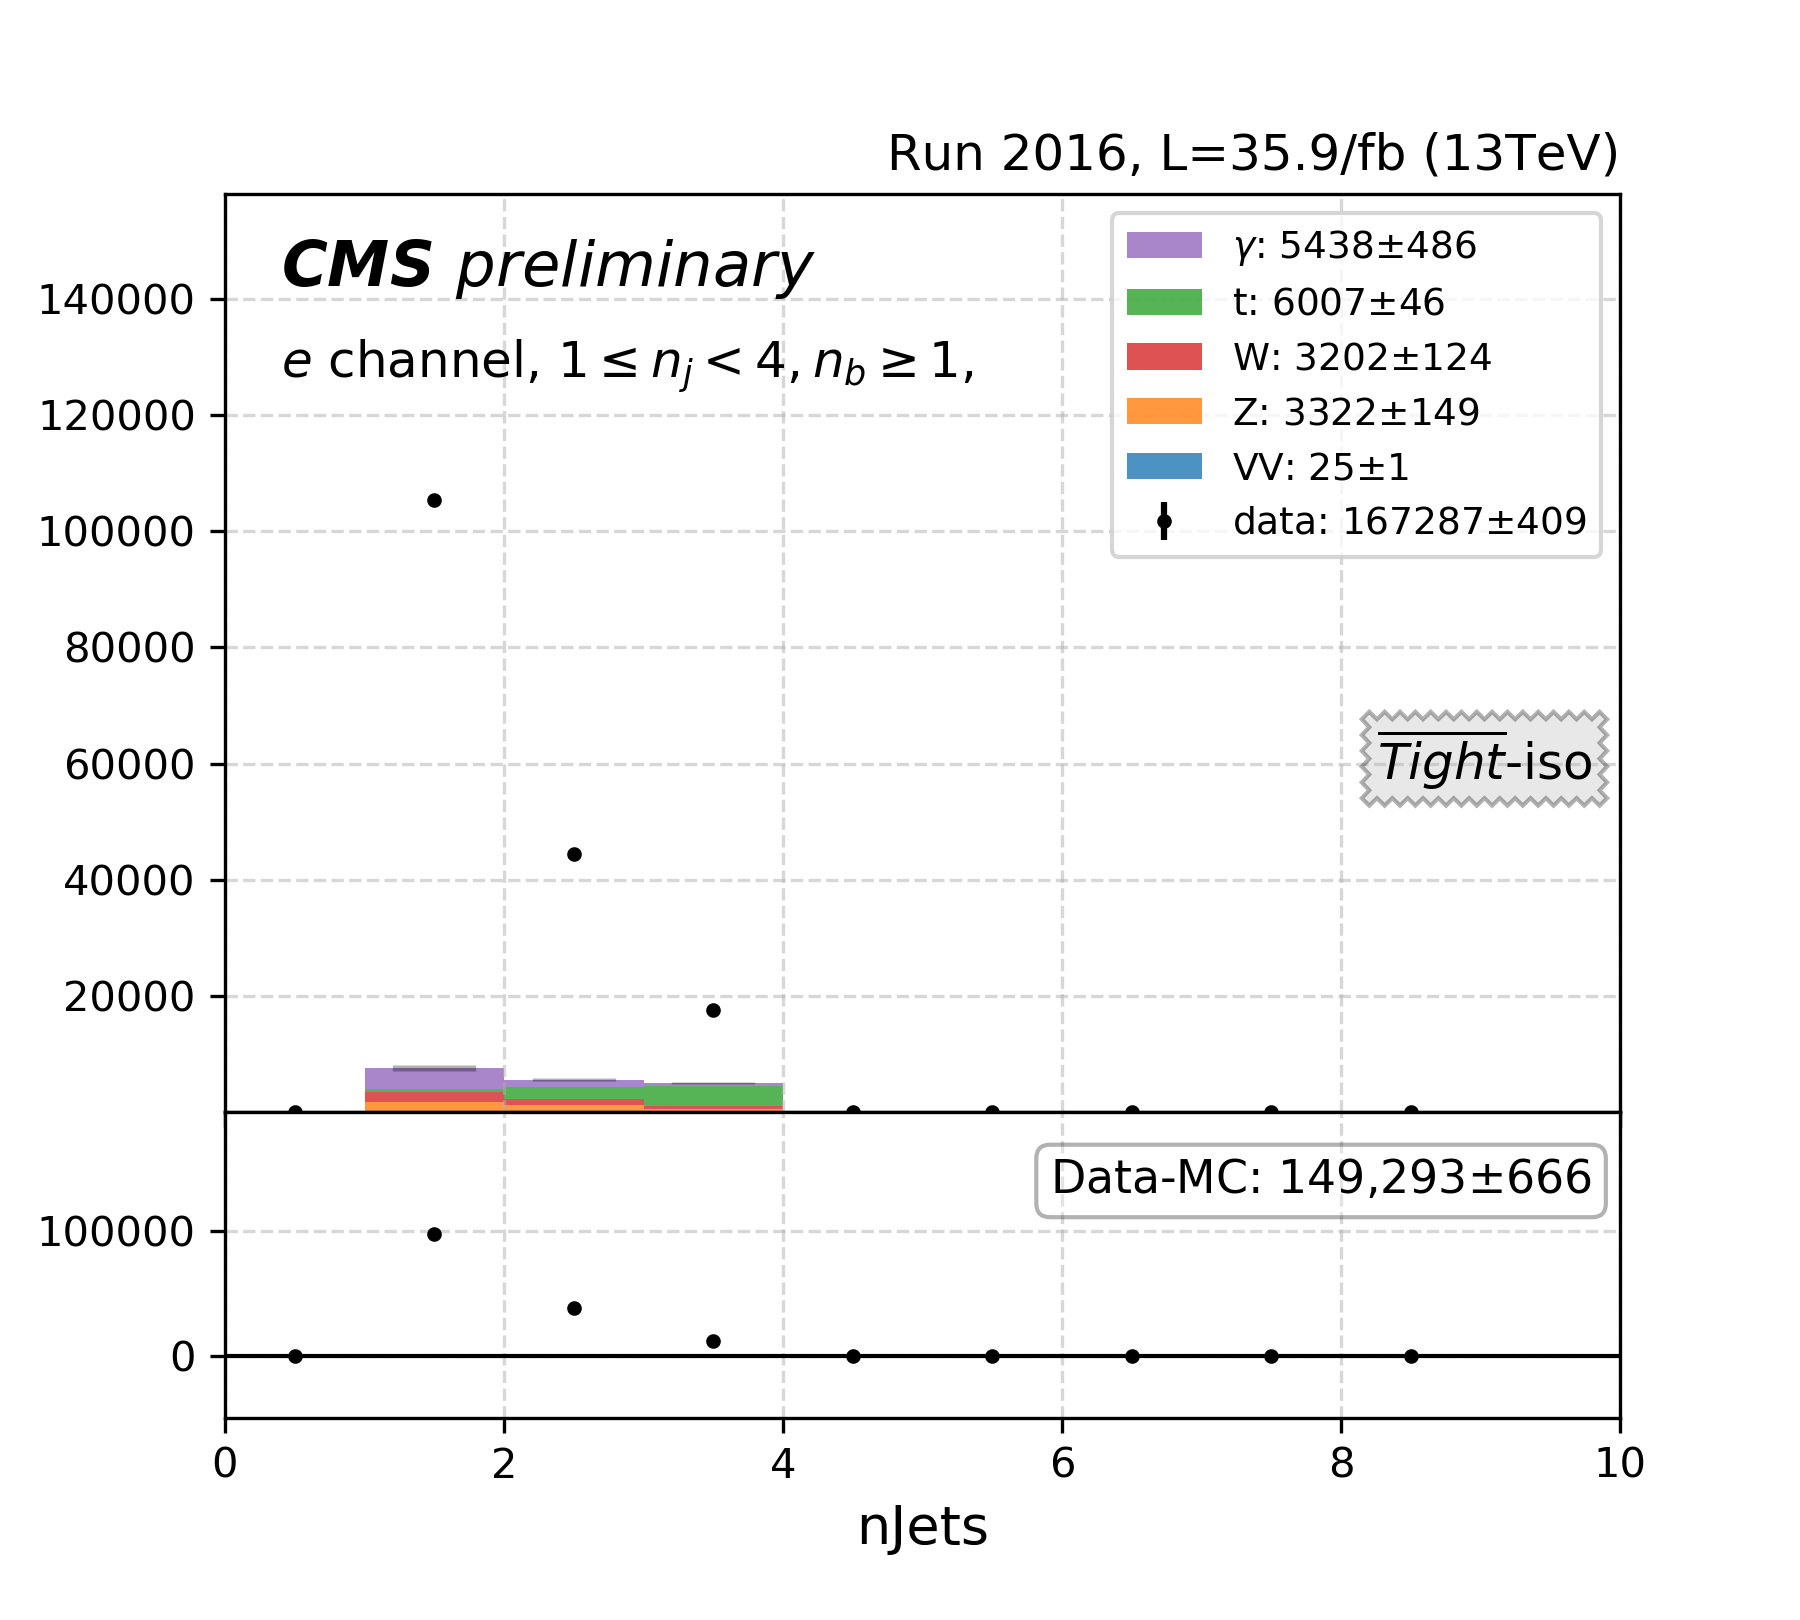
\includegraphics[width=0.24\textwidth]{chapters/Appendix/sectionQCD/figures/123j1b/e_nJets_False.png}
    
    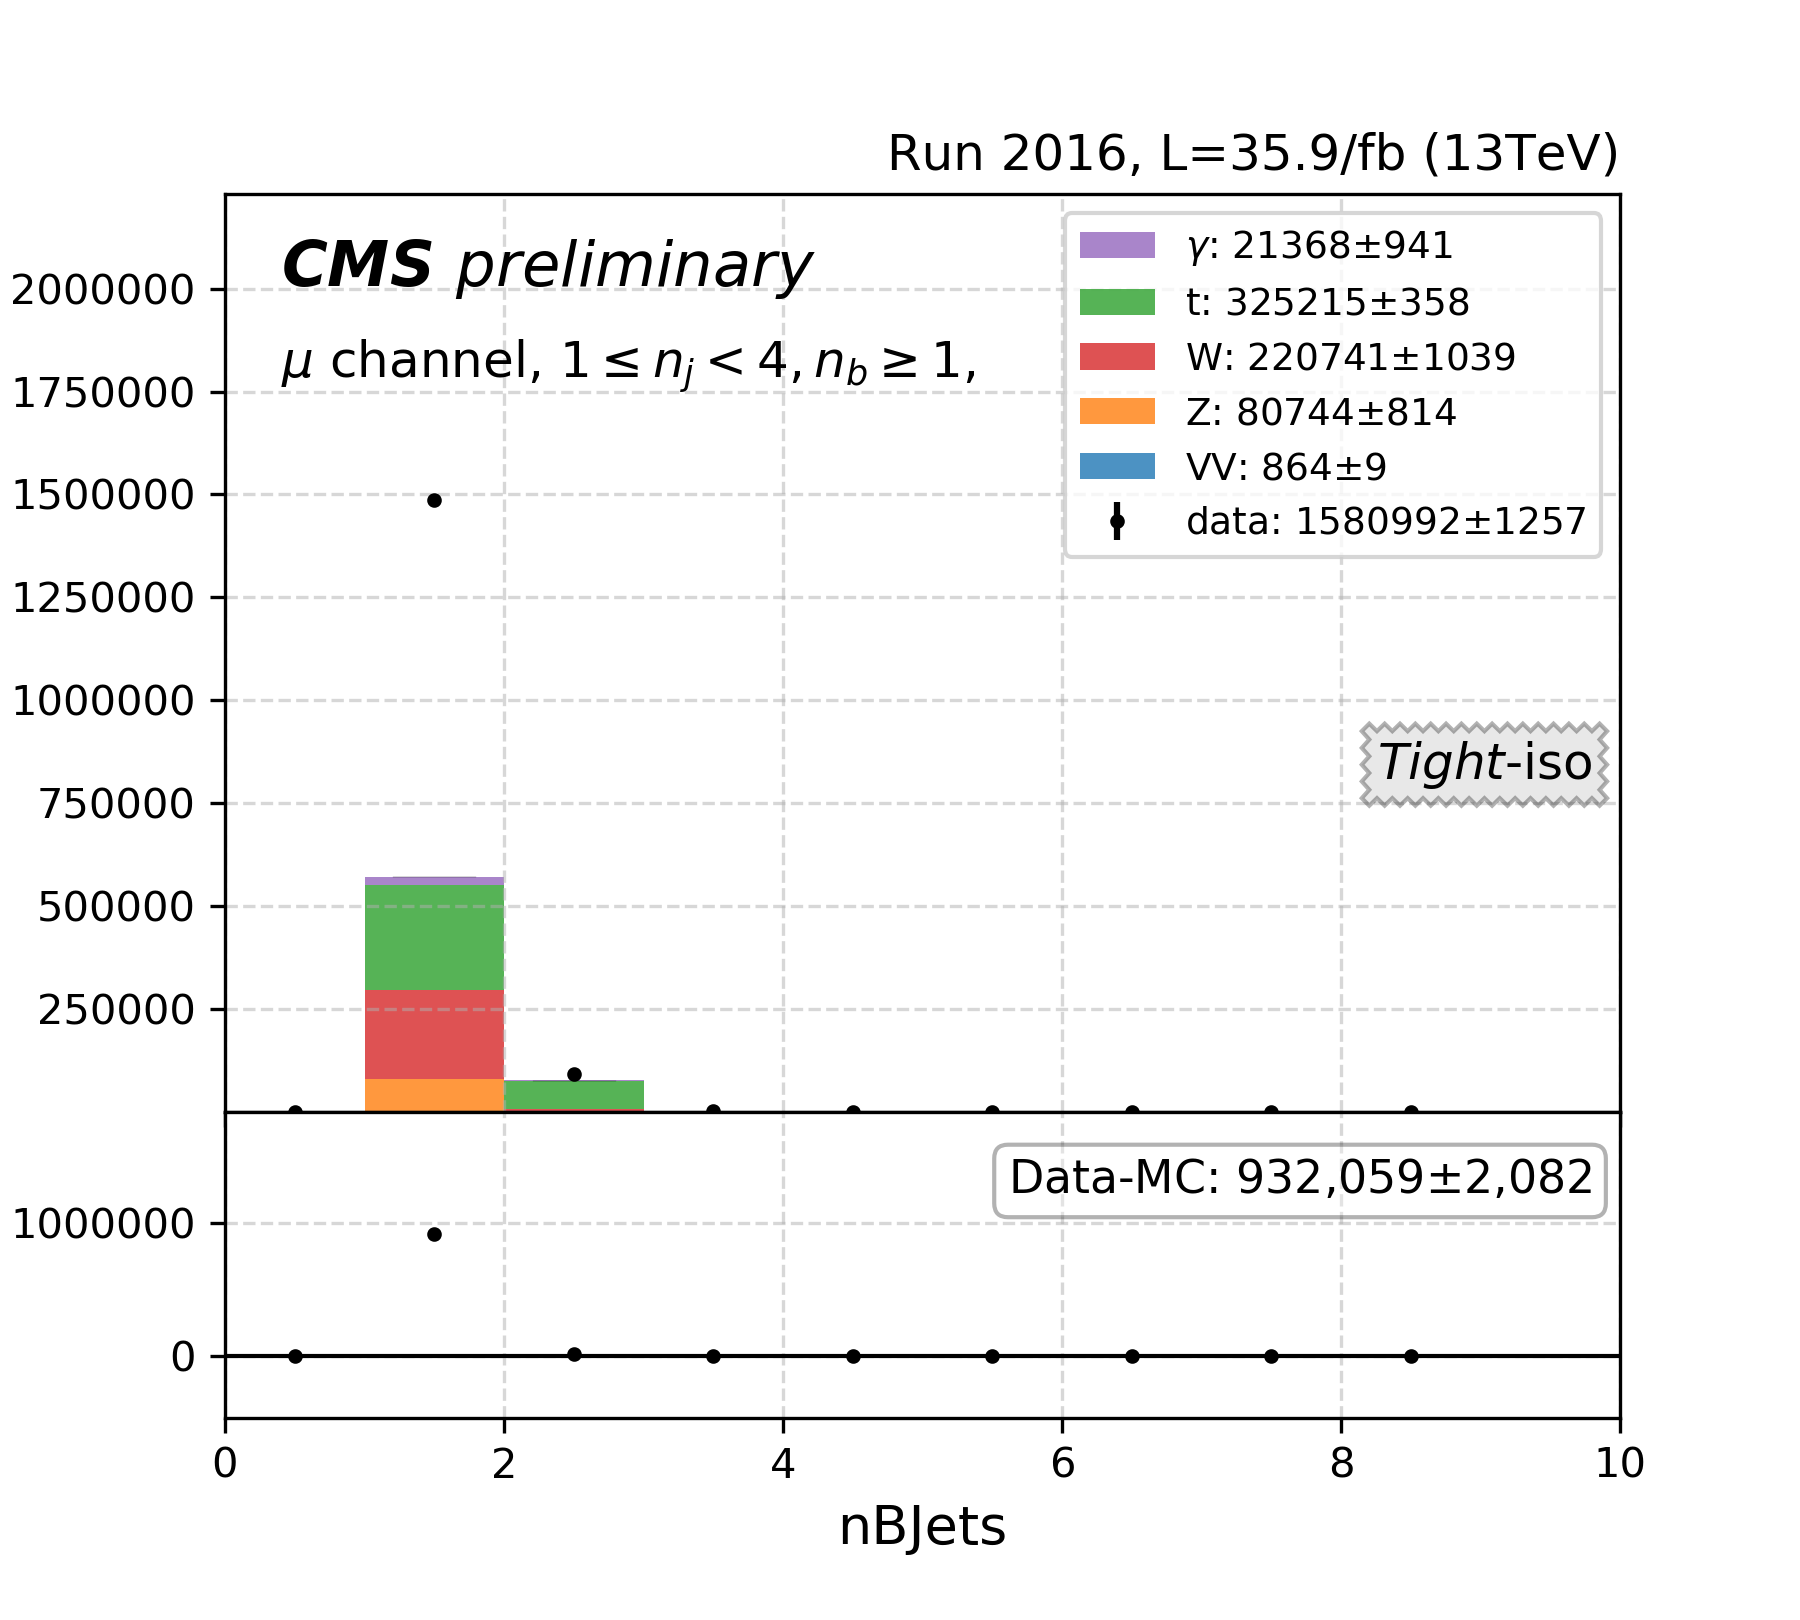
\includegraphics[width=0.24\textwidth]{chapters/Appendix/sectionQCD/figures/123j1b/mu_nBJets_True.png}
    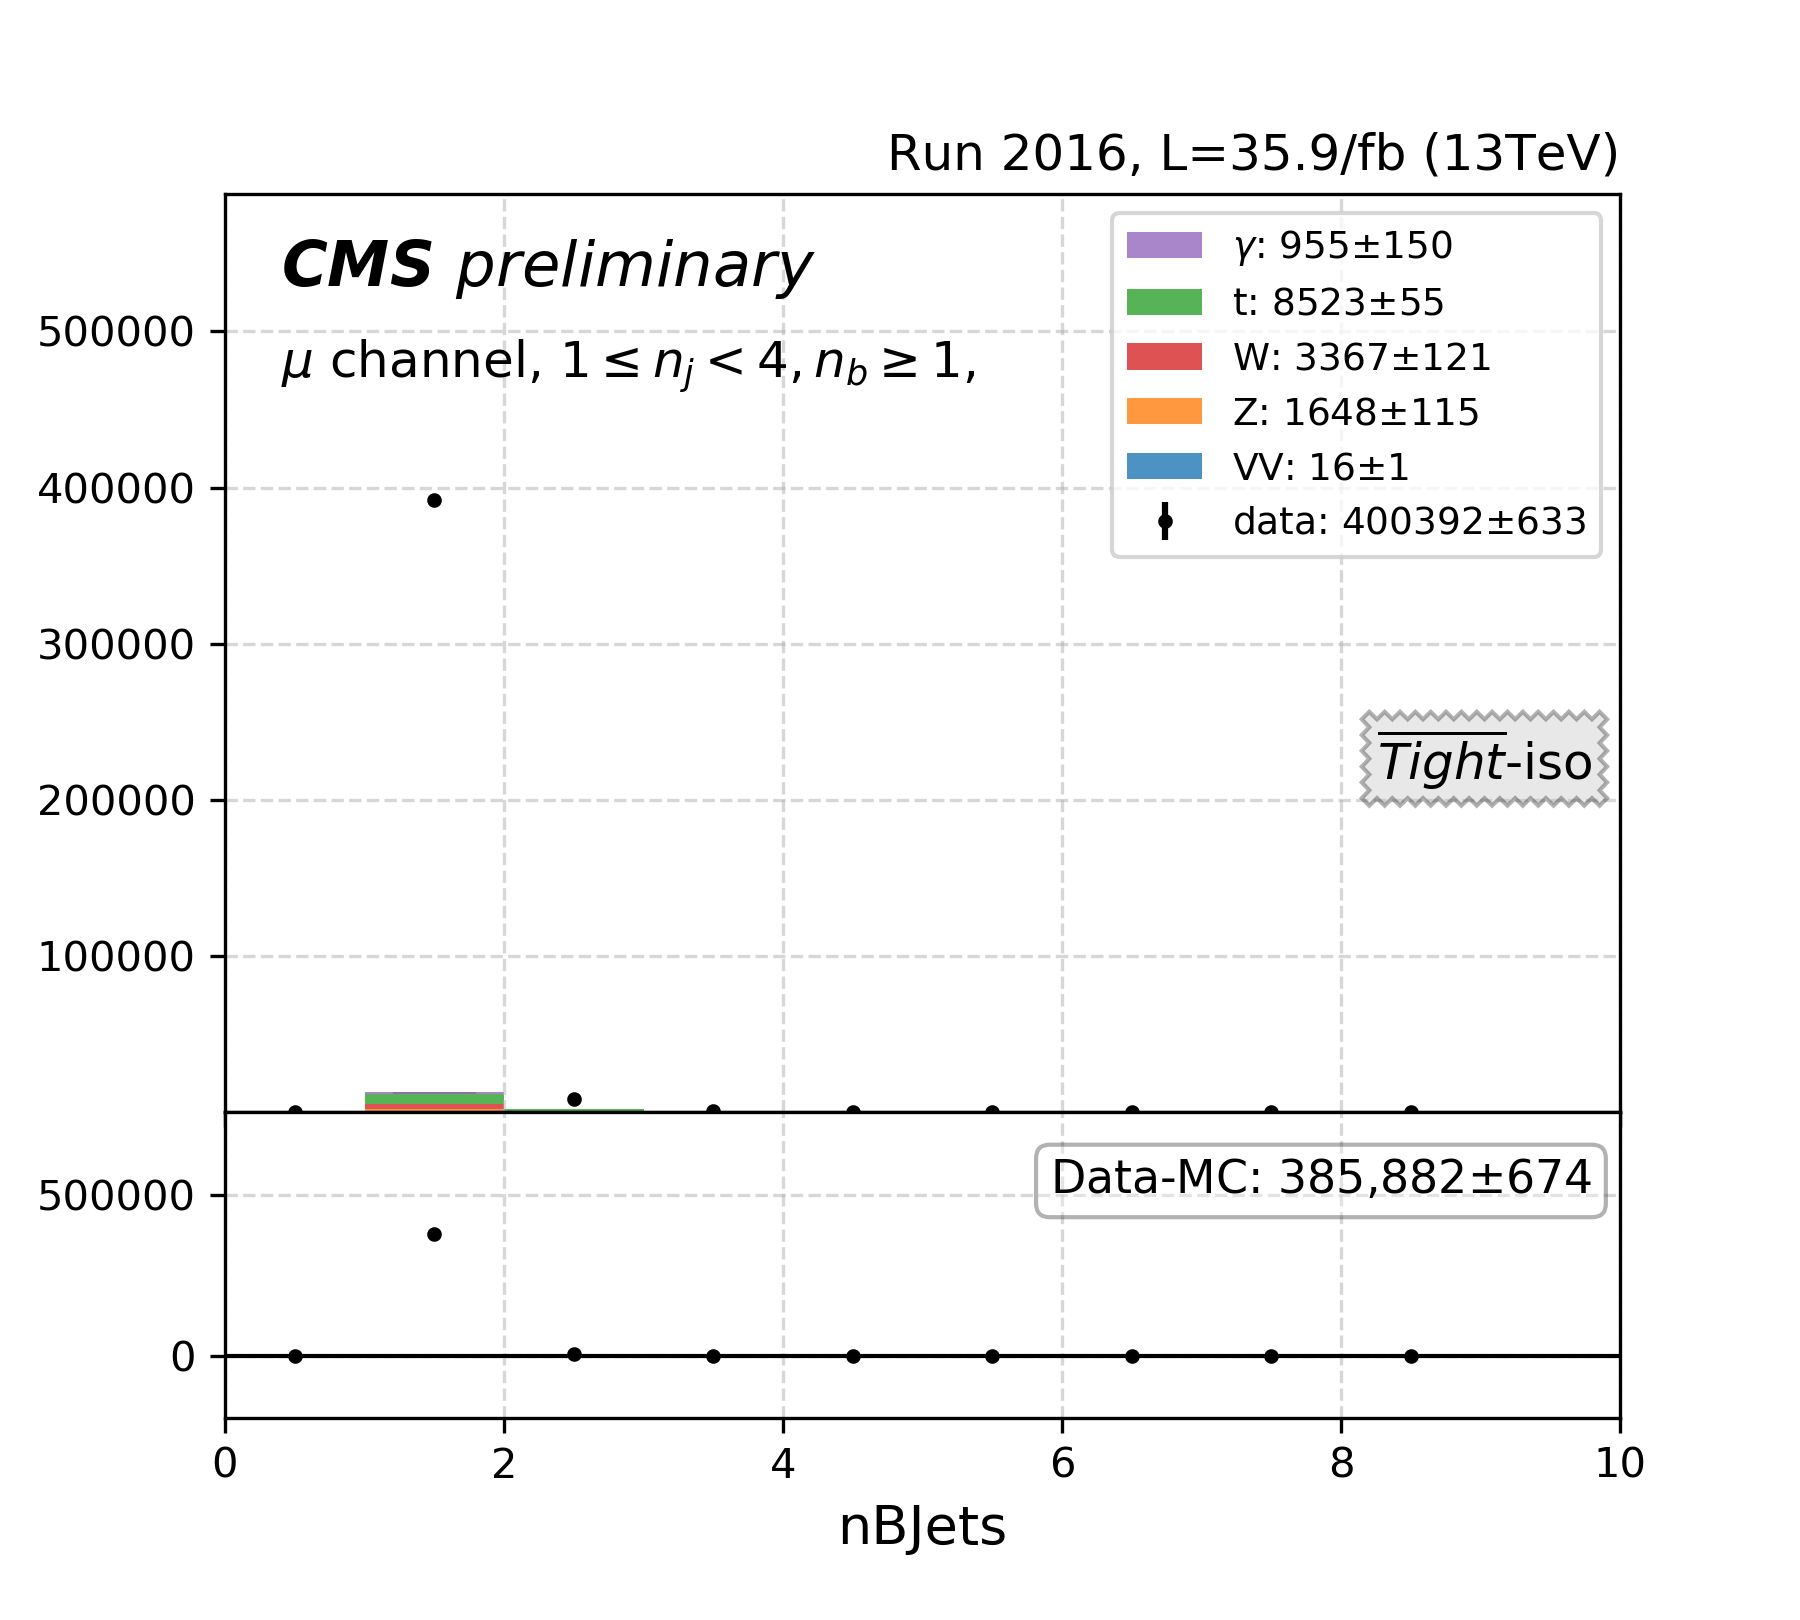
\includegraphics[width=0.24\textwidth]{chapters/Appendix/sectionQCD/figures/123j1b/mu_nBJets_False.png}
    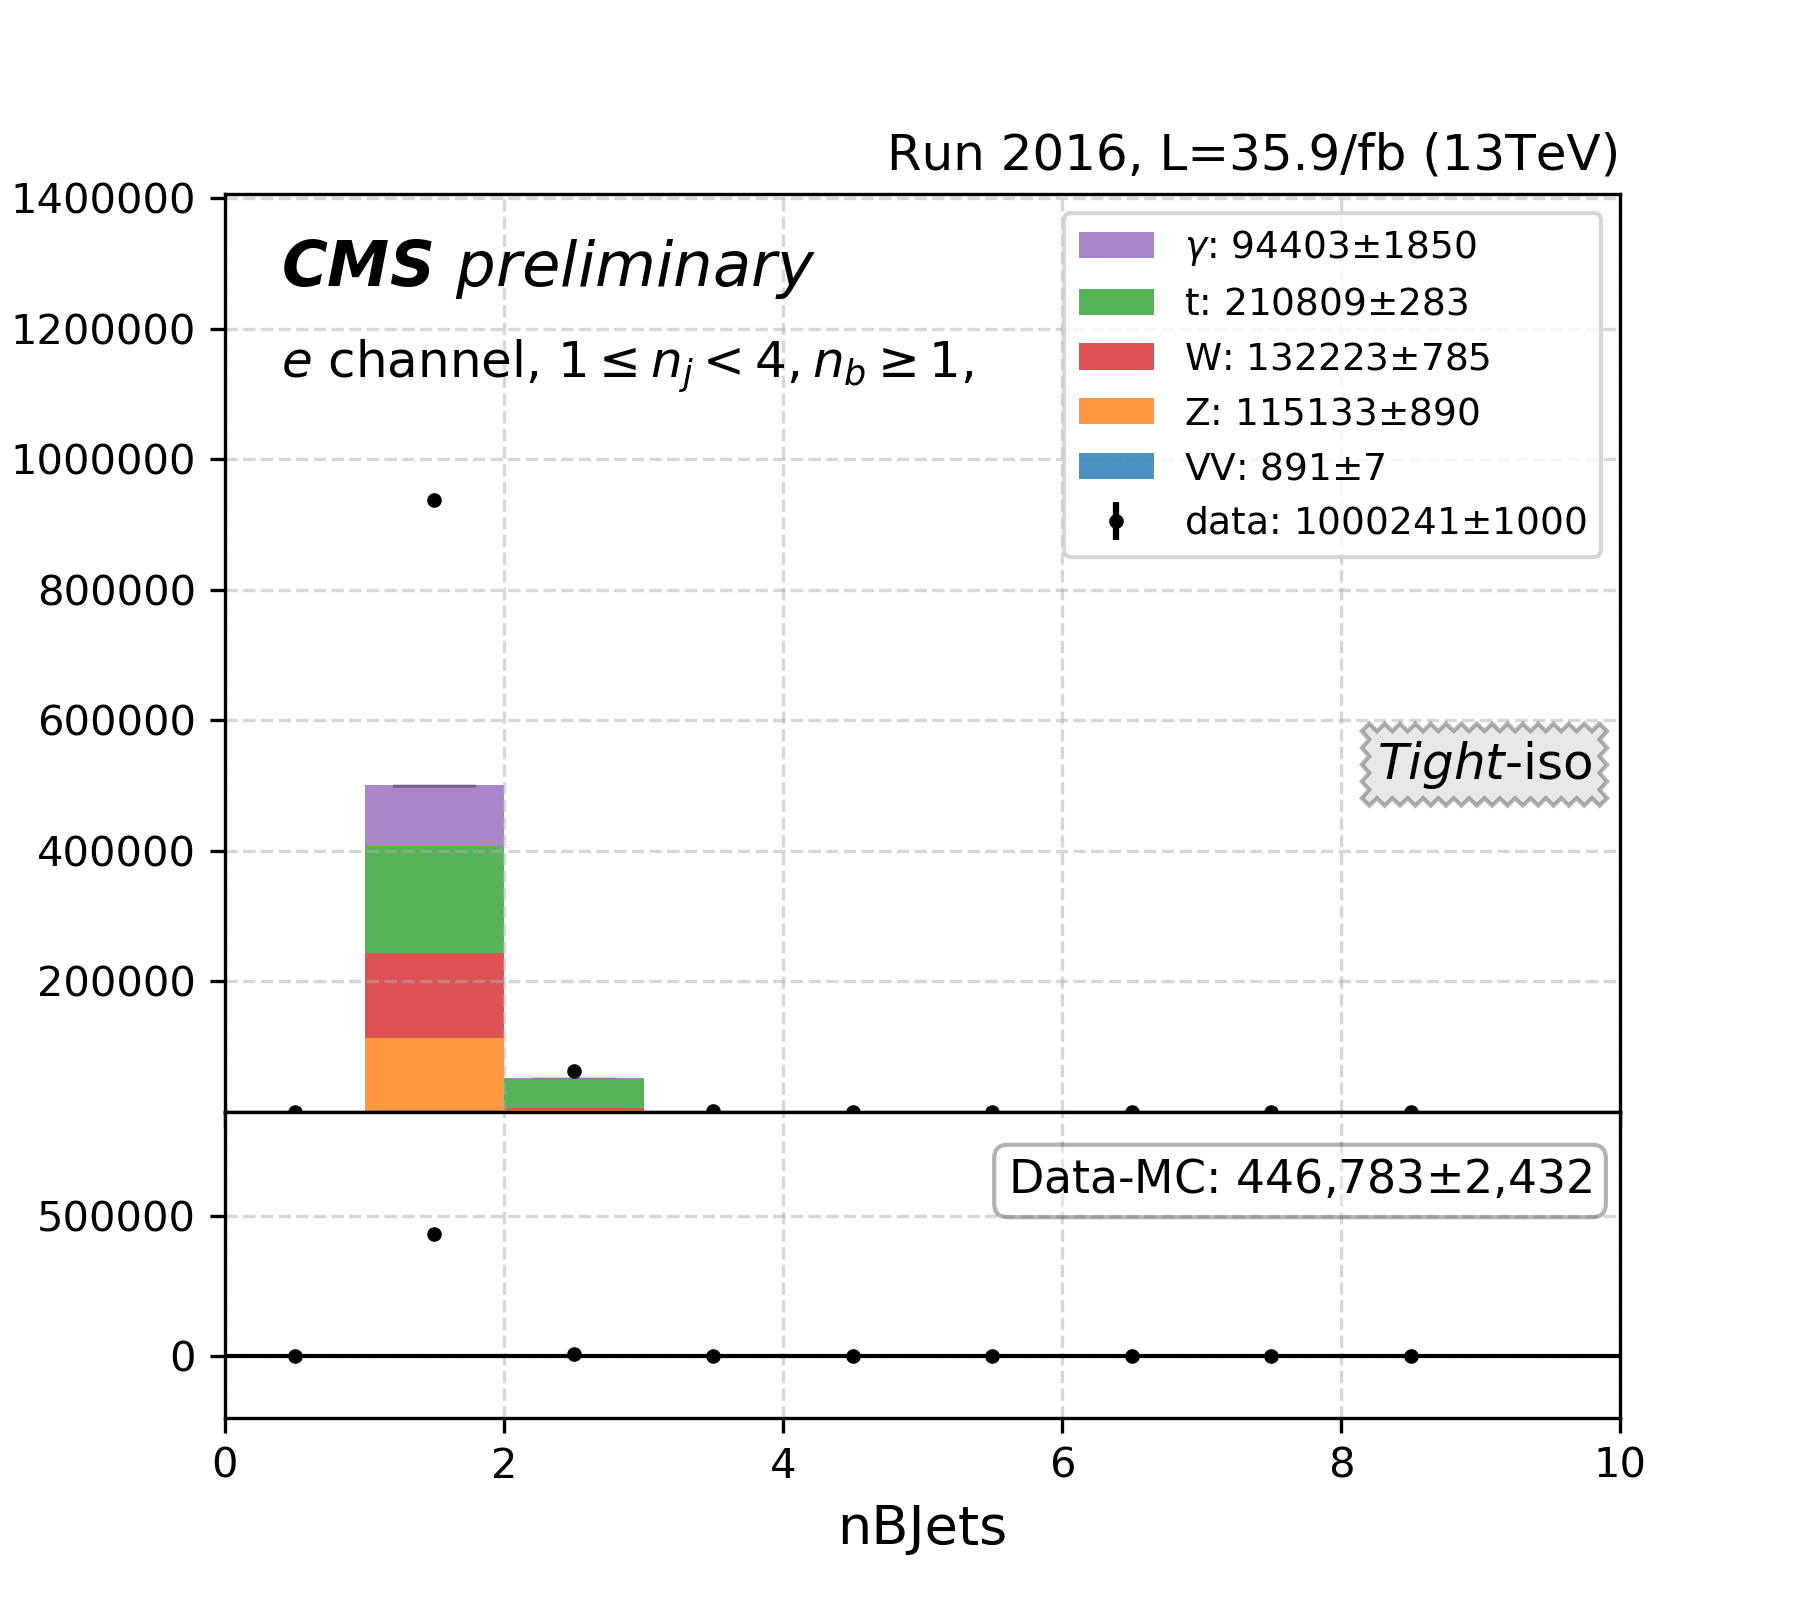
\includegraphics[width=0.24\textwidth]{chapters/Appendix/sectionQCD/figures/123j1b/e_nBJets_True.png}
    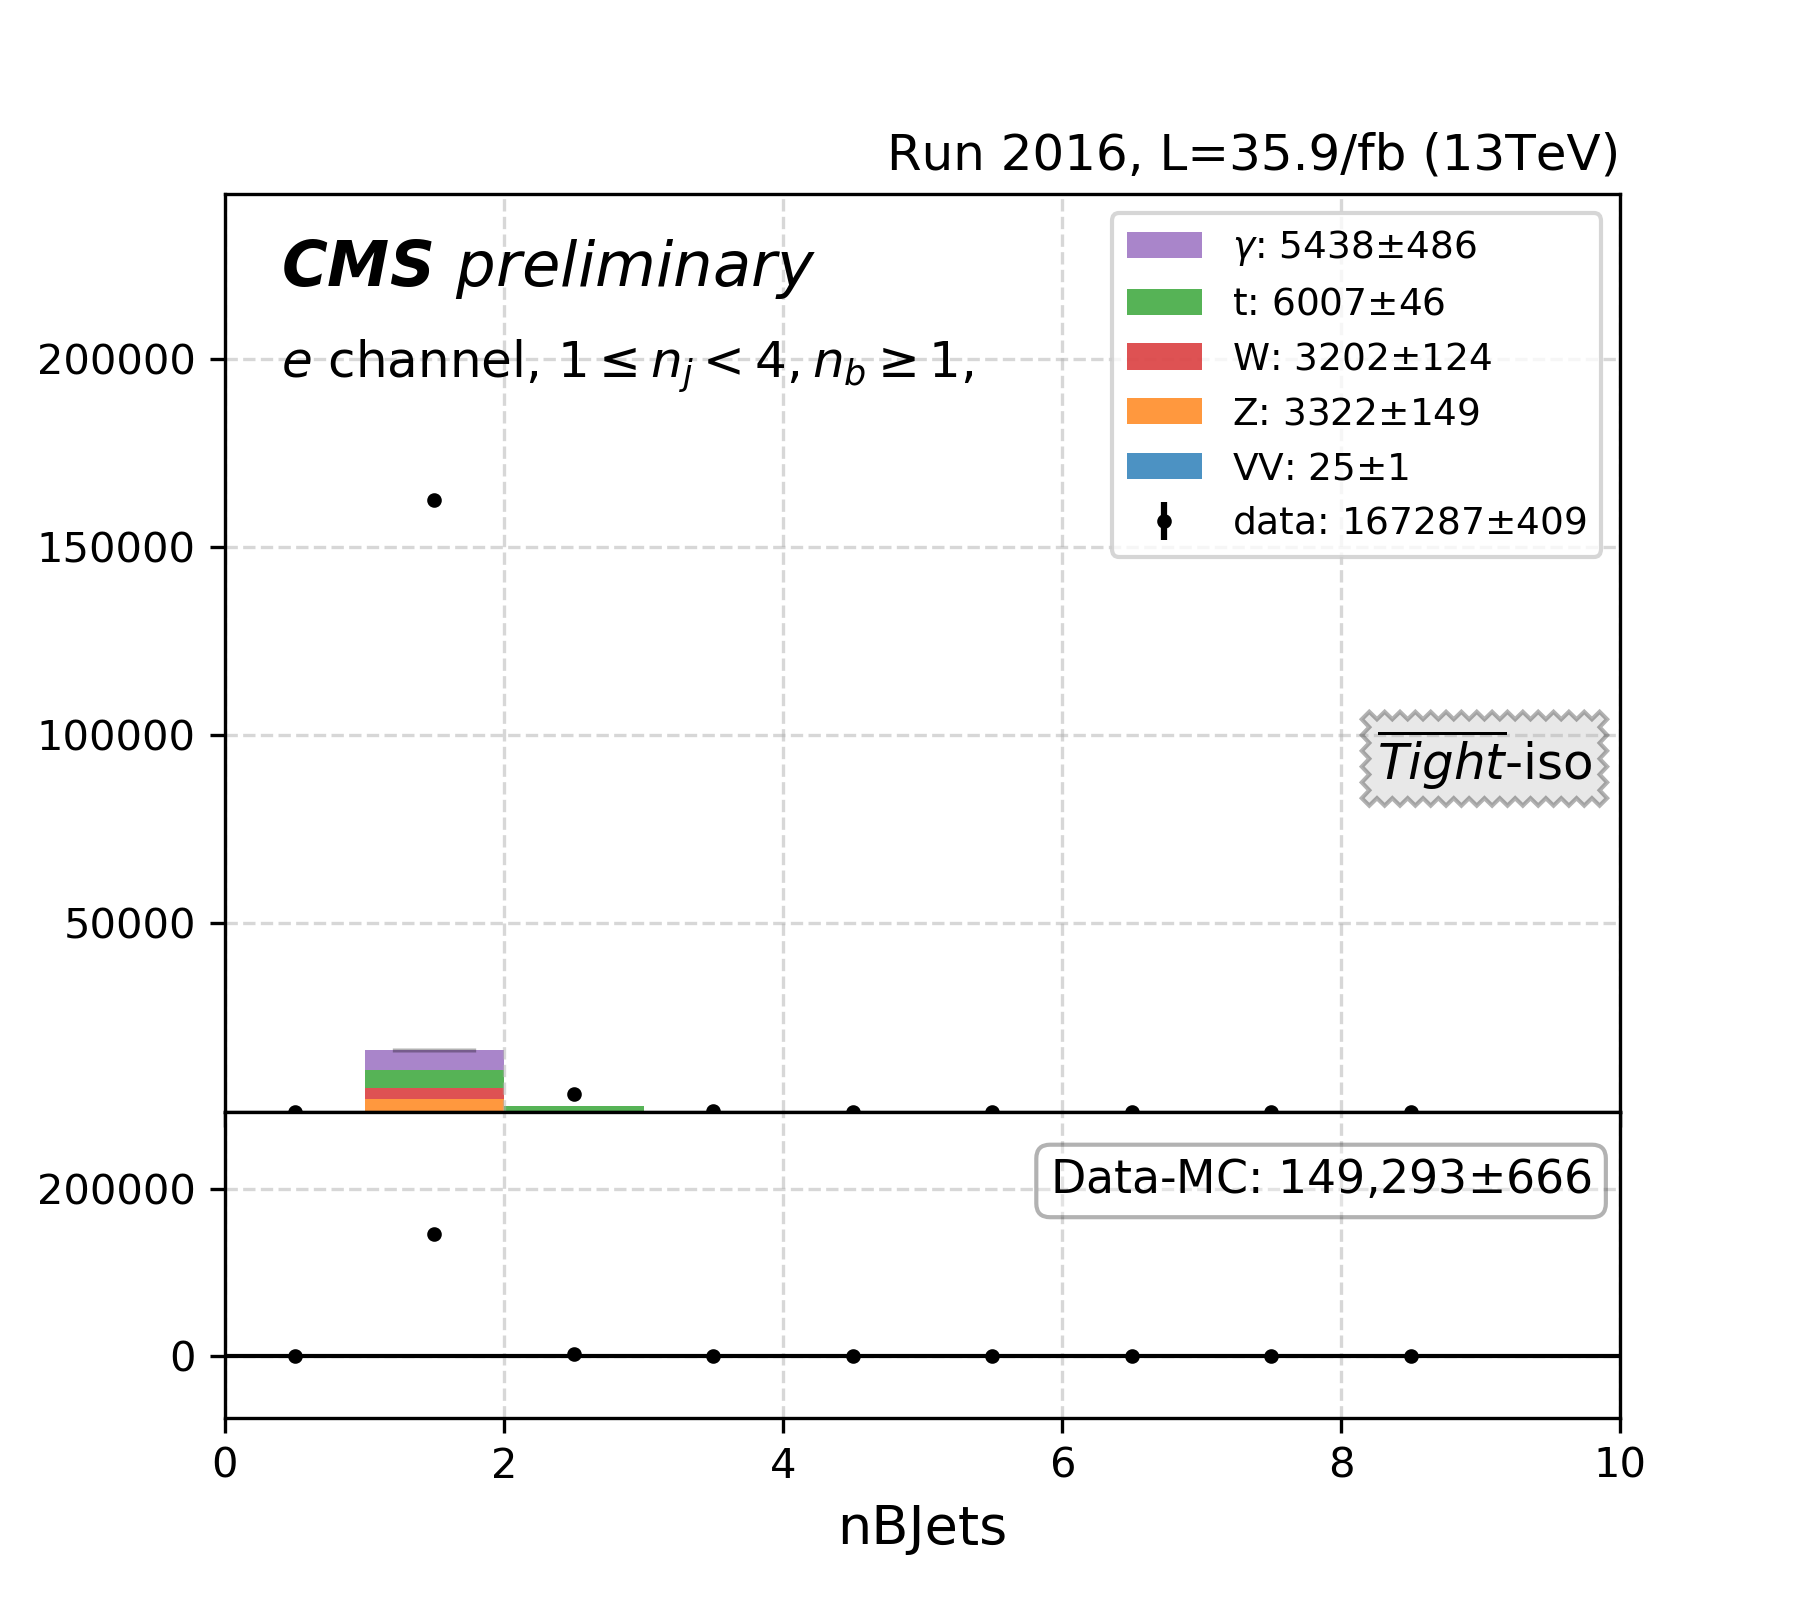
\includegraphics[width=0.24\textwidth]{chapters/Appendix/sectionQCD/figures/123j1b/e_nBJets_False.png}
    

    \caption{The iso and anti-iso region of $\mu$+jet (left two columns) and $e$+jet (right two columns) channel 
    with $1\leq n_j <4, n_b\geq1$, which is orthogonal to the $n_j\geq4,n_b\geq1$ signal region.
    }
    \label{fig:appendix:123j1b}
\end{figure}


\begin{figure}
    \centering
    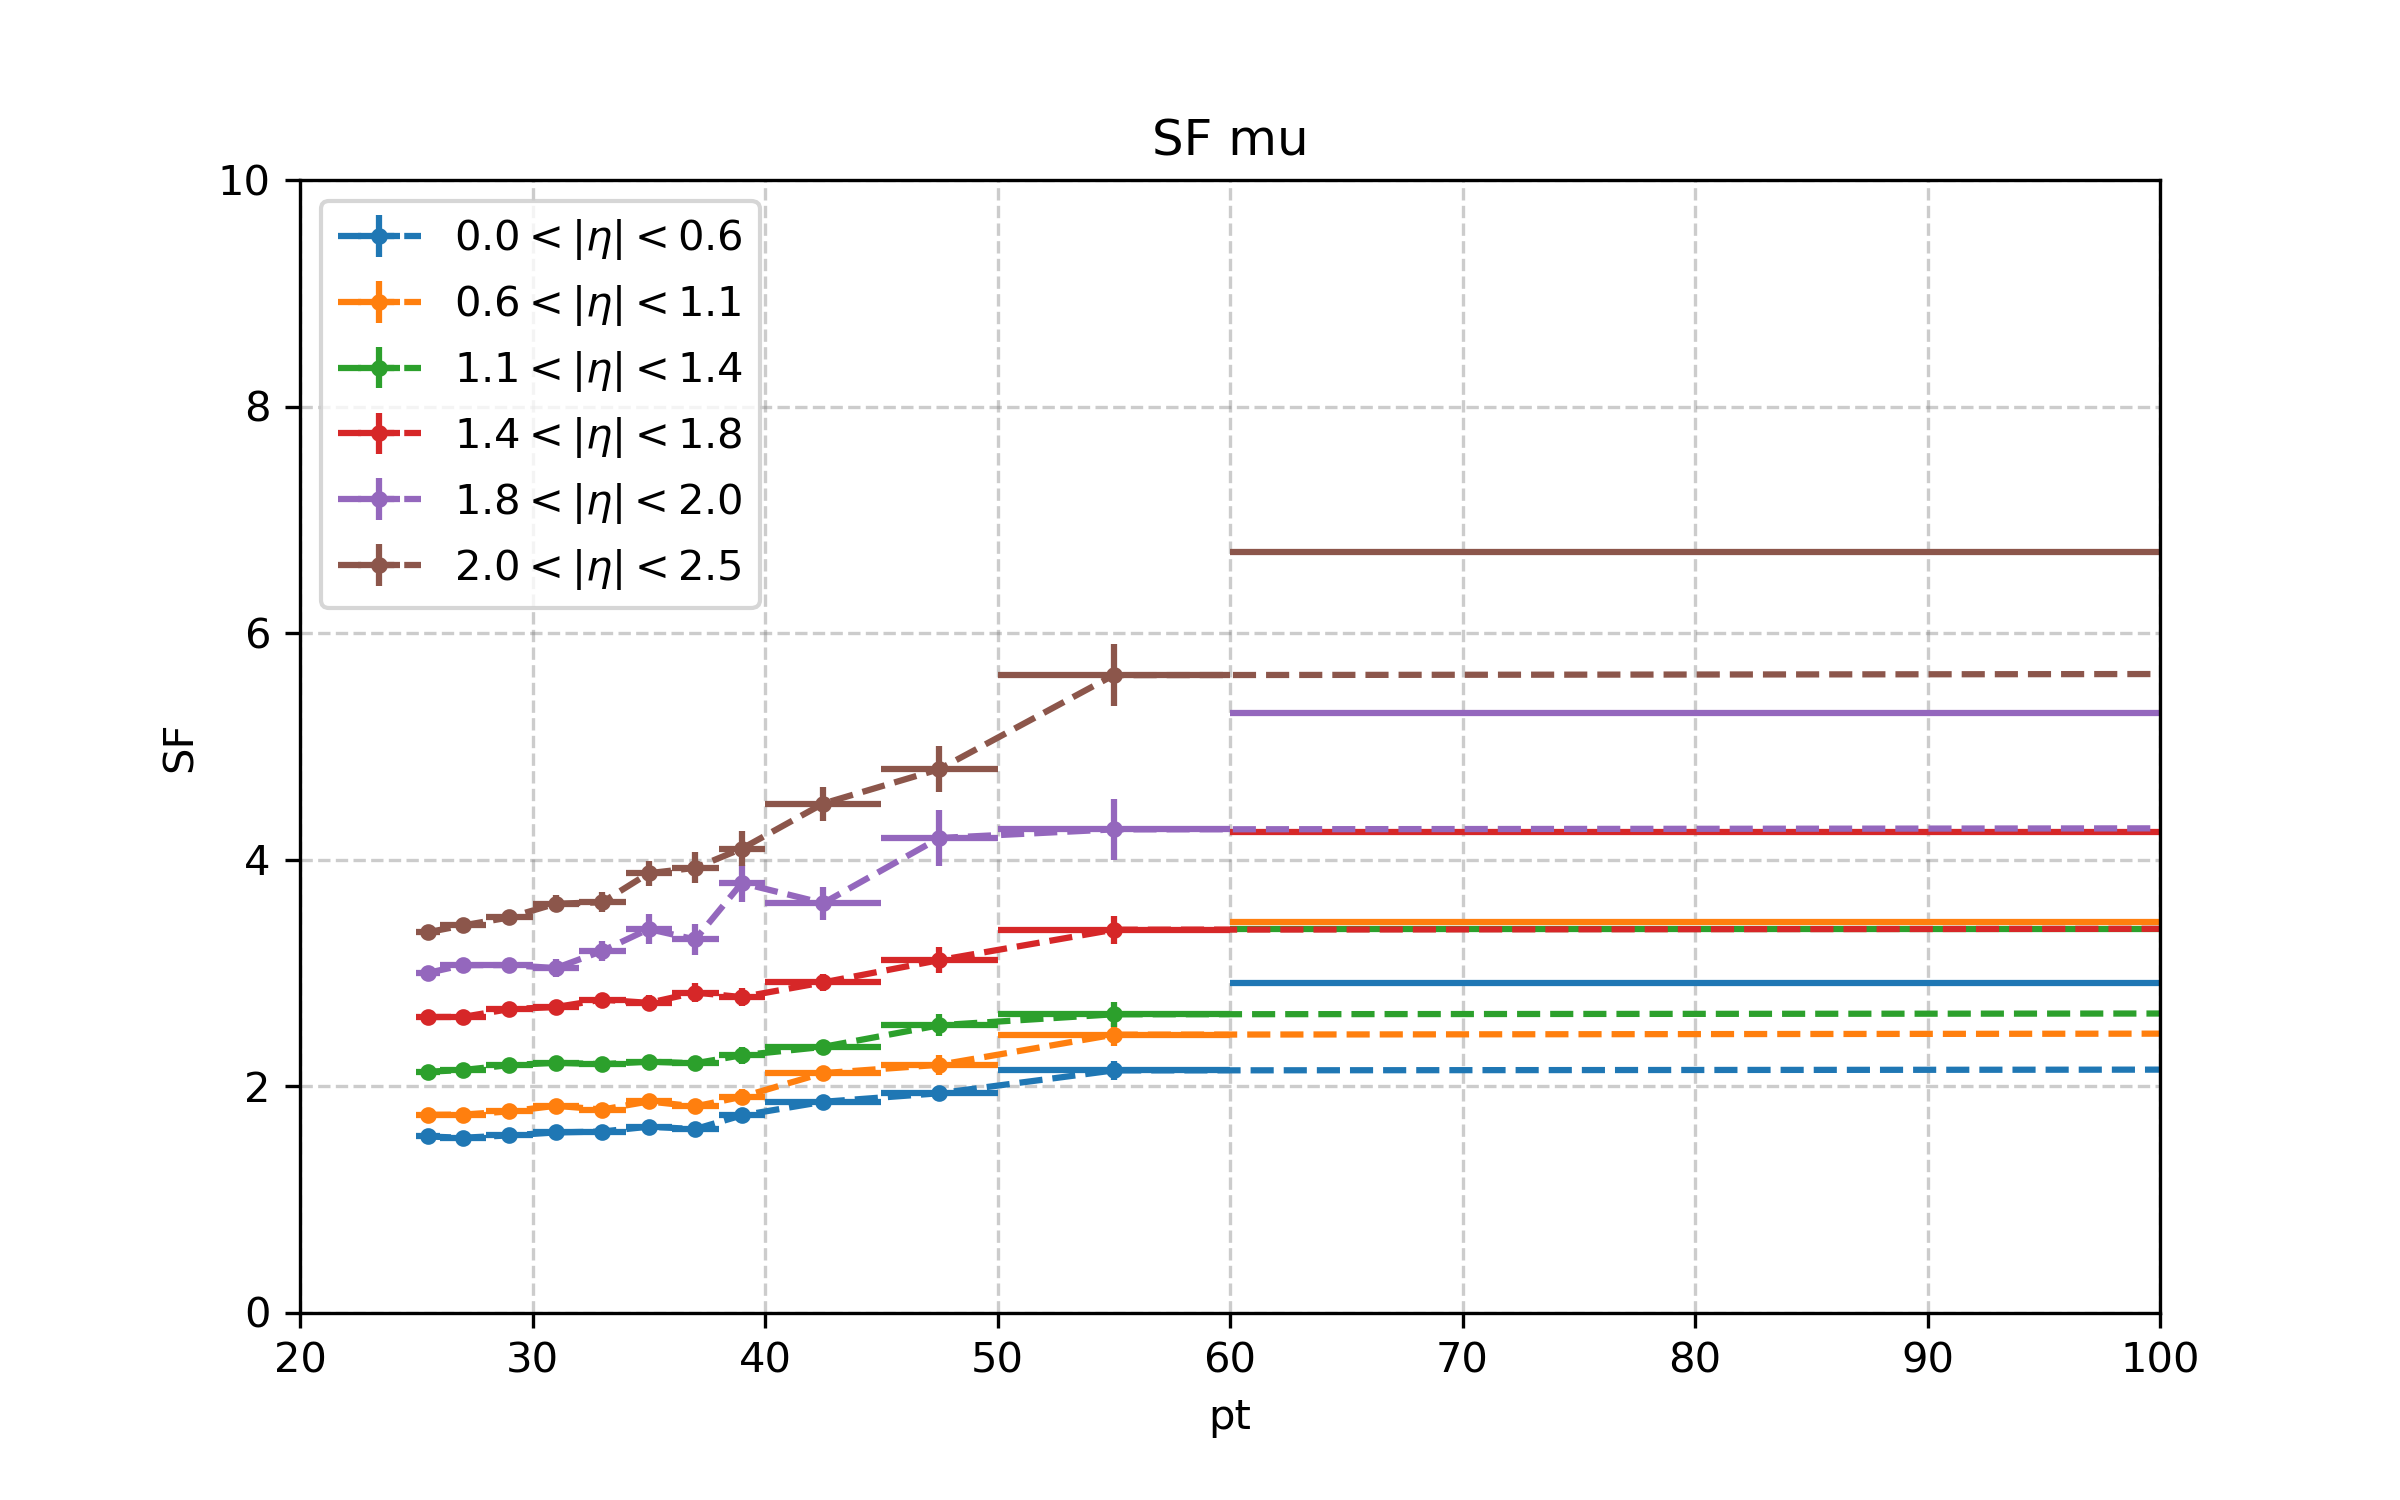
\includegraphics[width=0.49\textwidth]{chapters/Appendix/sectionQCD/figures/123j1b/SF_mu_1d.png}
    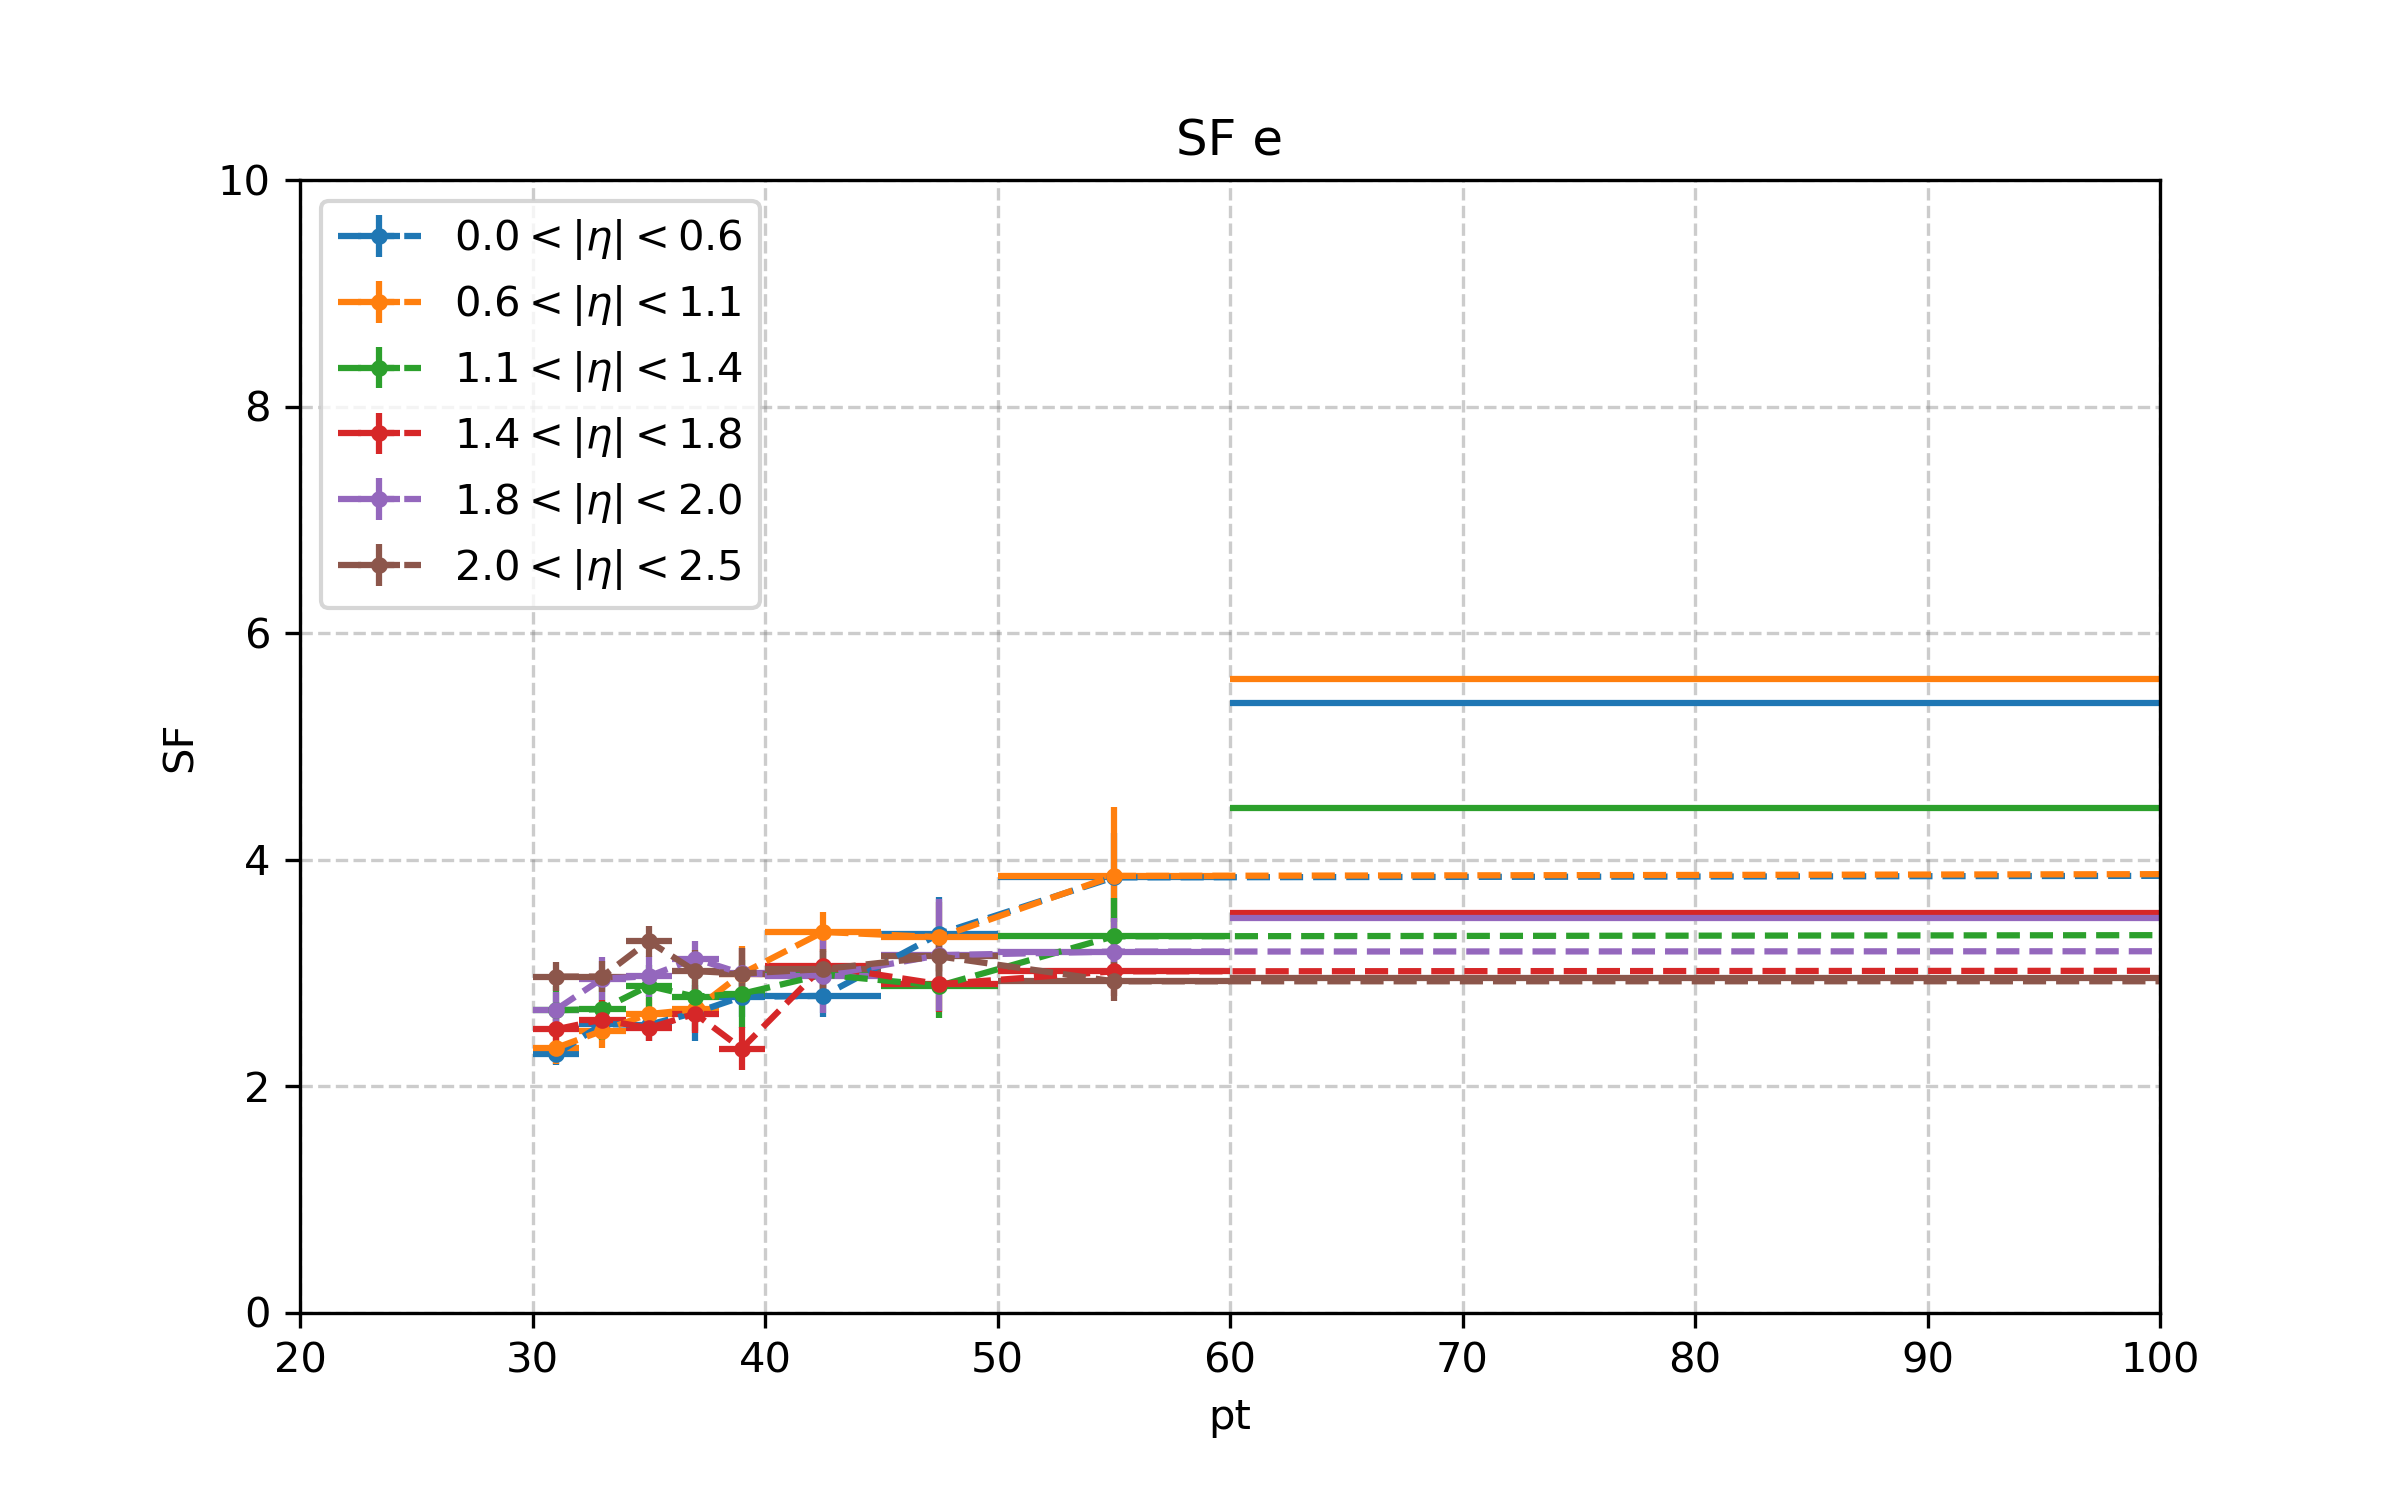
\includegraphics[width=0.49\textwidth]{chapters/Appendix/sectionQCD/figures/123j1b/SF_e_1d.png}
    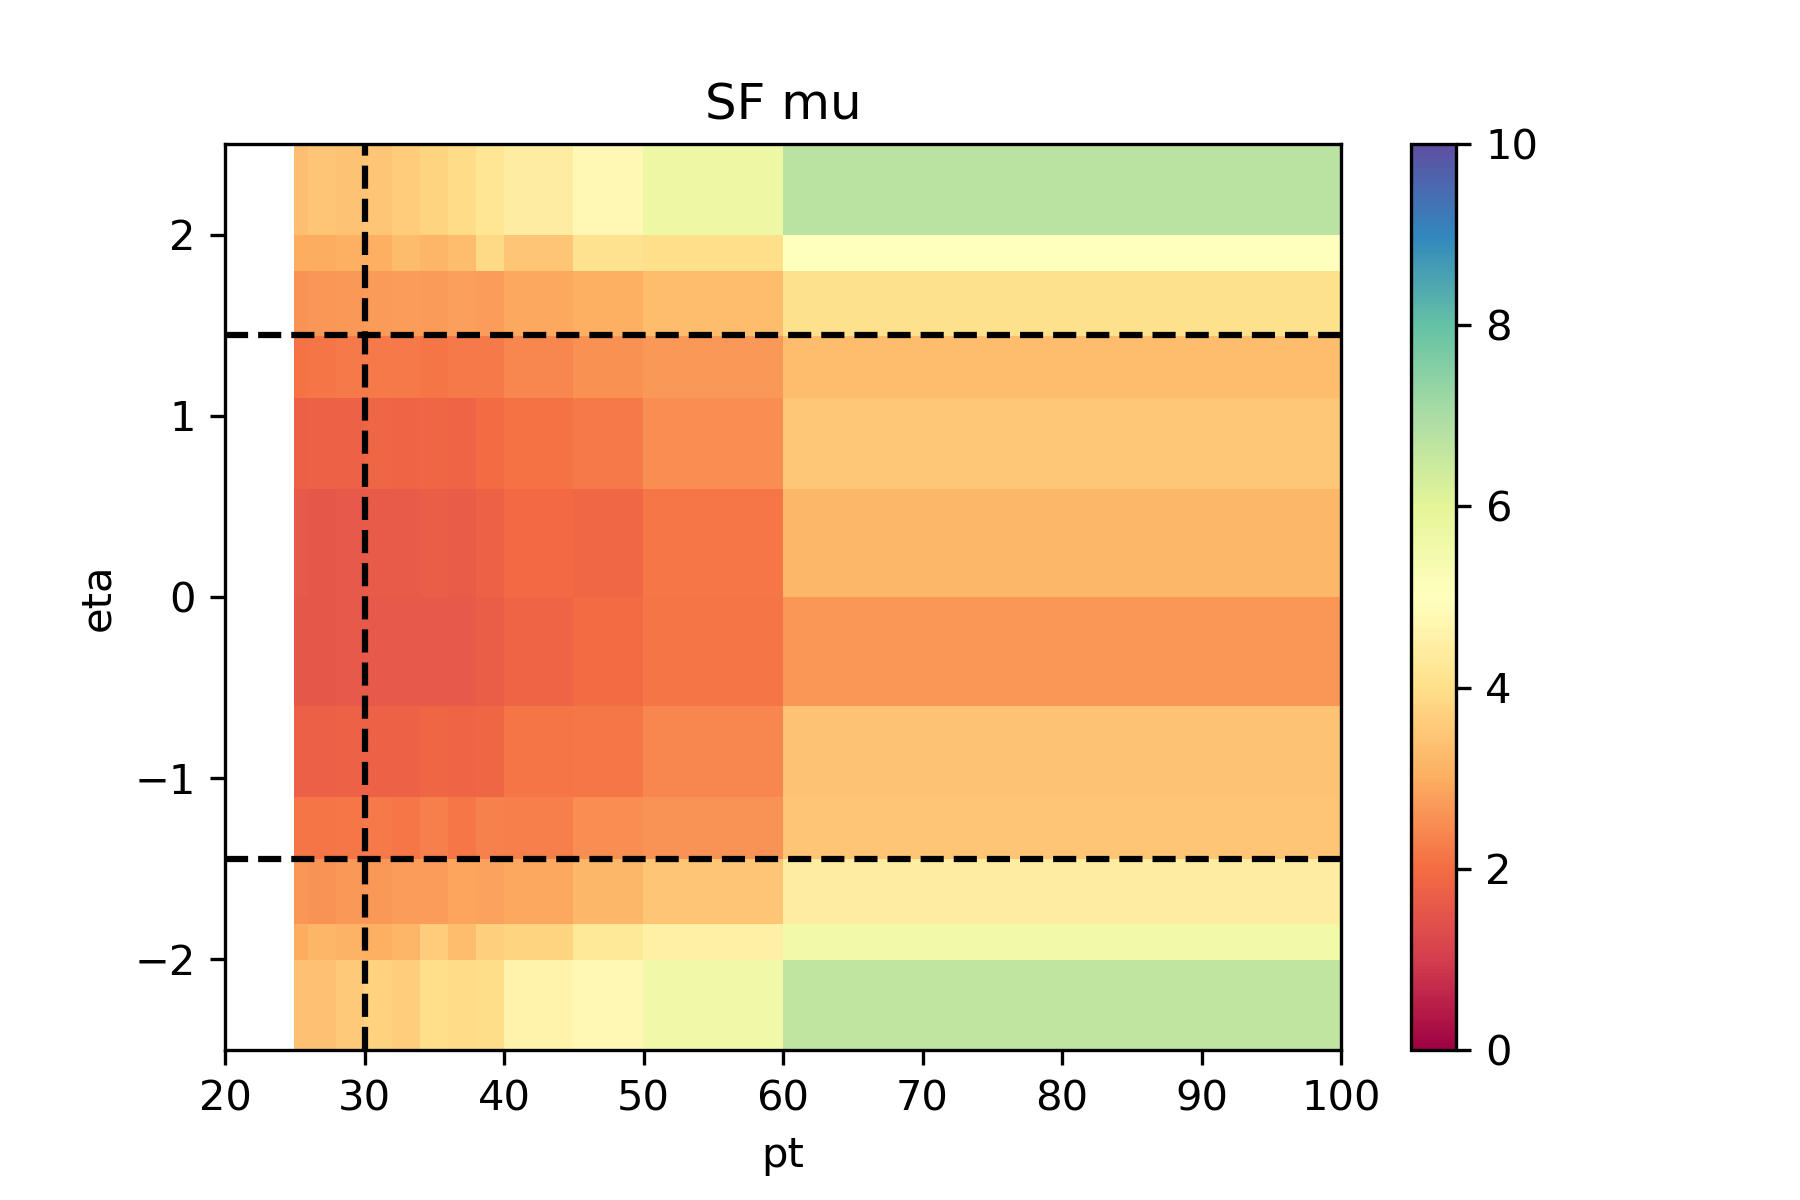
\includegraphics[width=0.49\textwidth]{chapters/Appendix/sectionQCD/figures/123j1b/SF_mu_2d.png}
    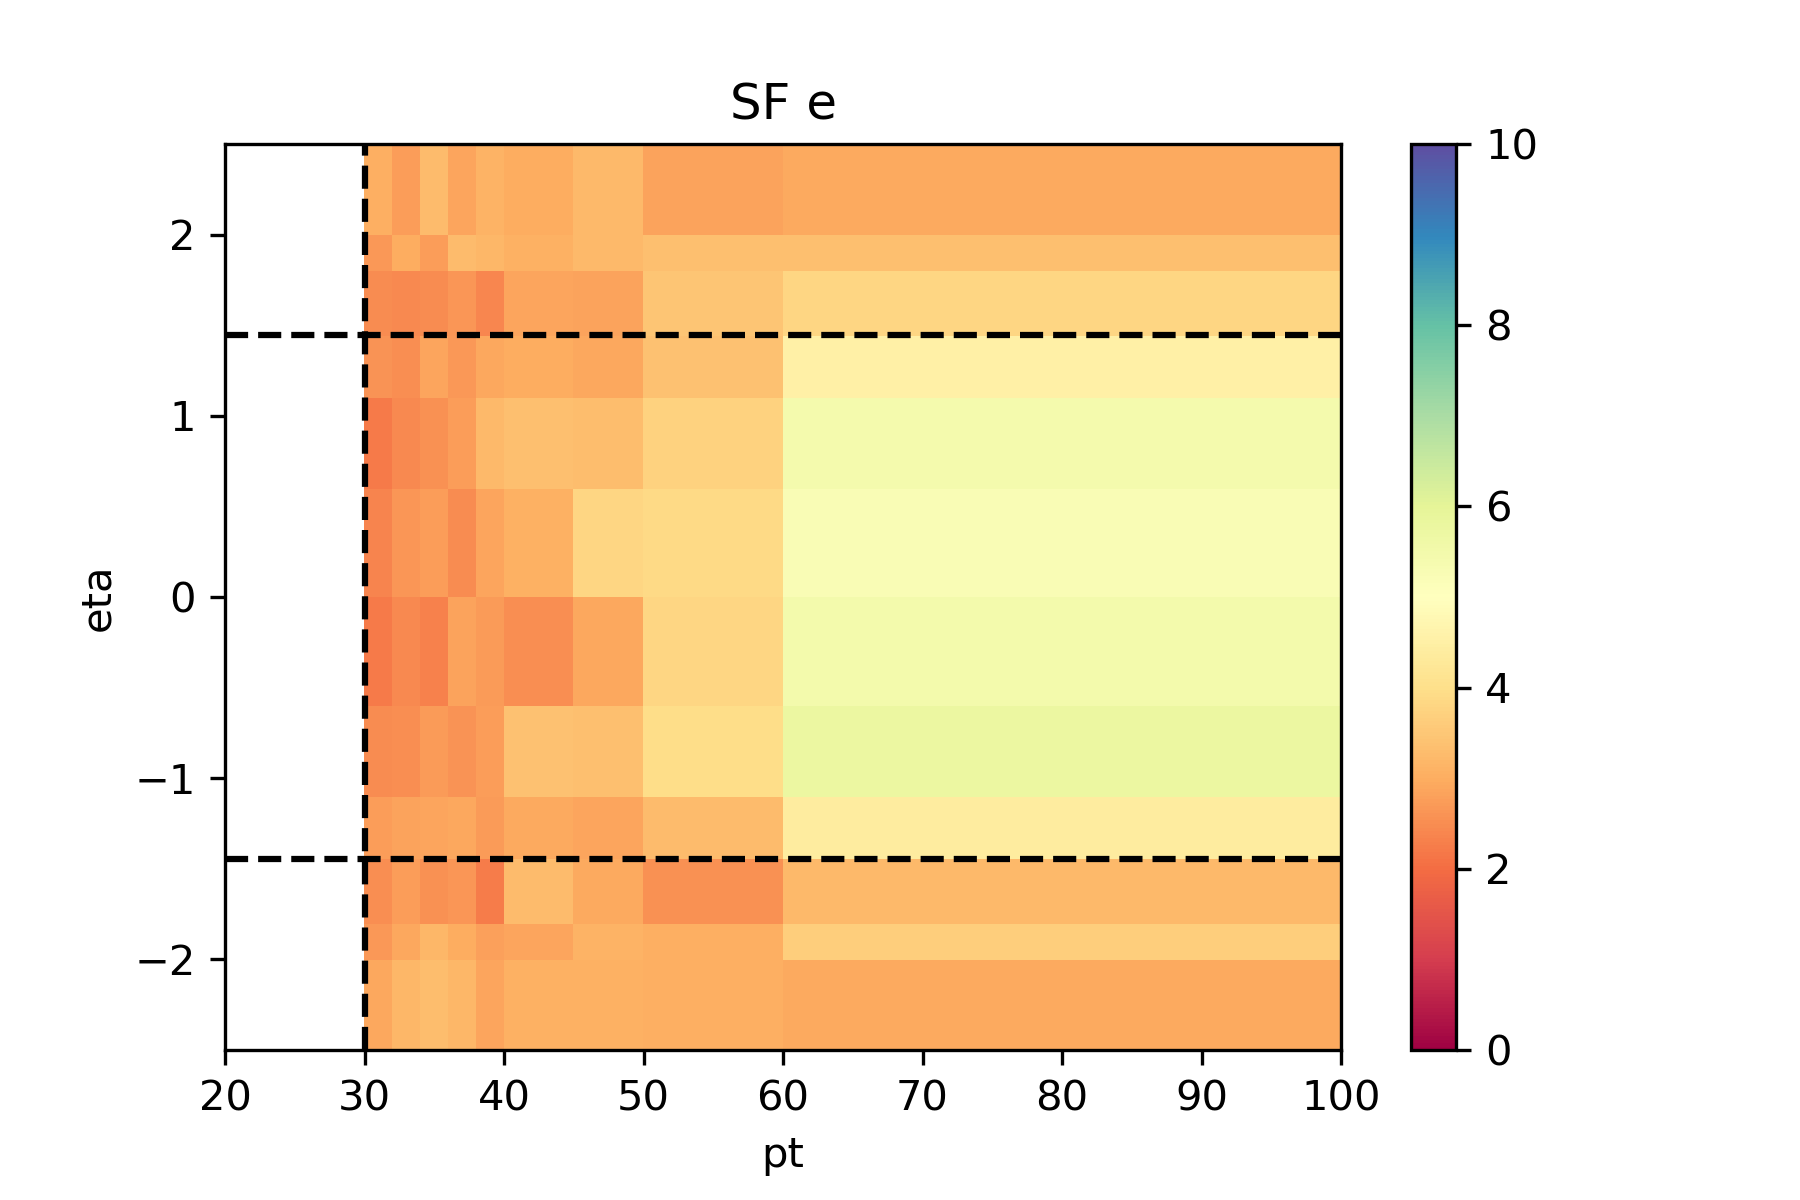
\includegraphics[width=0.49\textwidth]{chapters/Appendix/sectionQCD/figures/123j1b/SF_e_2d.png}

    \caption{iso-to-antiiso SF in the $\mu$+jet (left) and $e$+jet (right) channel 
    with $1\leq n_j <4, n_b\geq1$ side-band region.}
    \label{fig:appendix:123j1b_sf}
\end{figure}


In the second approach, the HT-binned QCD MC is used. Figure~\ref{fig:appendix:4j1b} shows iso and antiiso region of $\mu$jet (left two columns) and $e$jet (right two columns) channel
with $n_j\geq4,n_b\geq1$ and the QCD MC in the signal region is shown as red line.

\begin{figure}
    \centering
    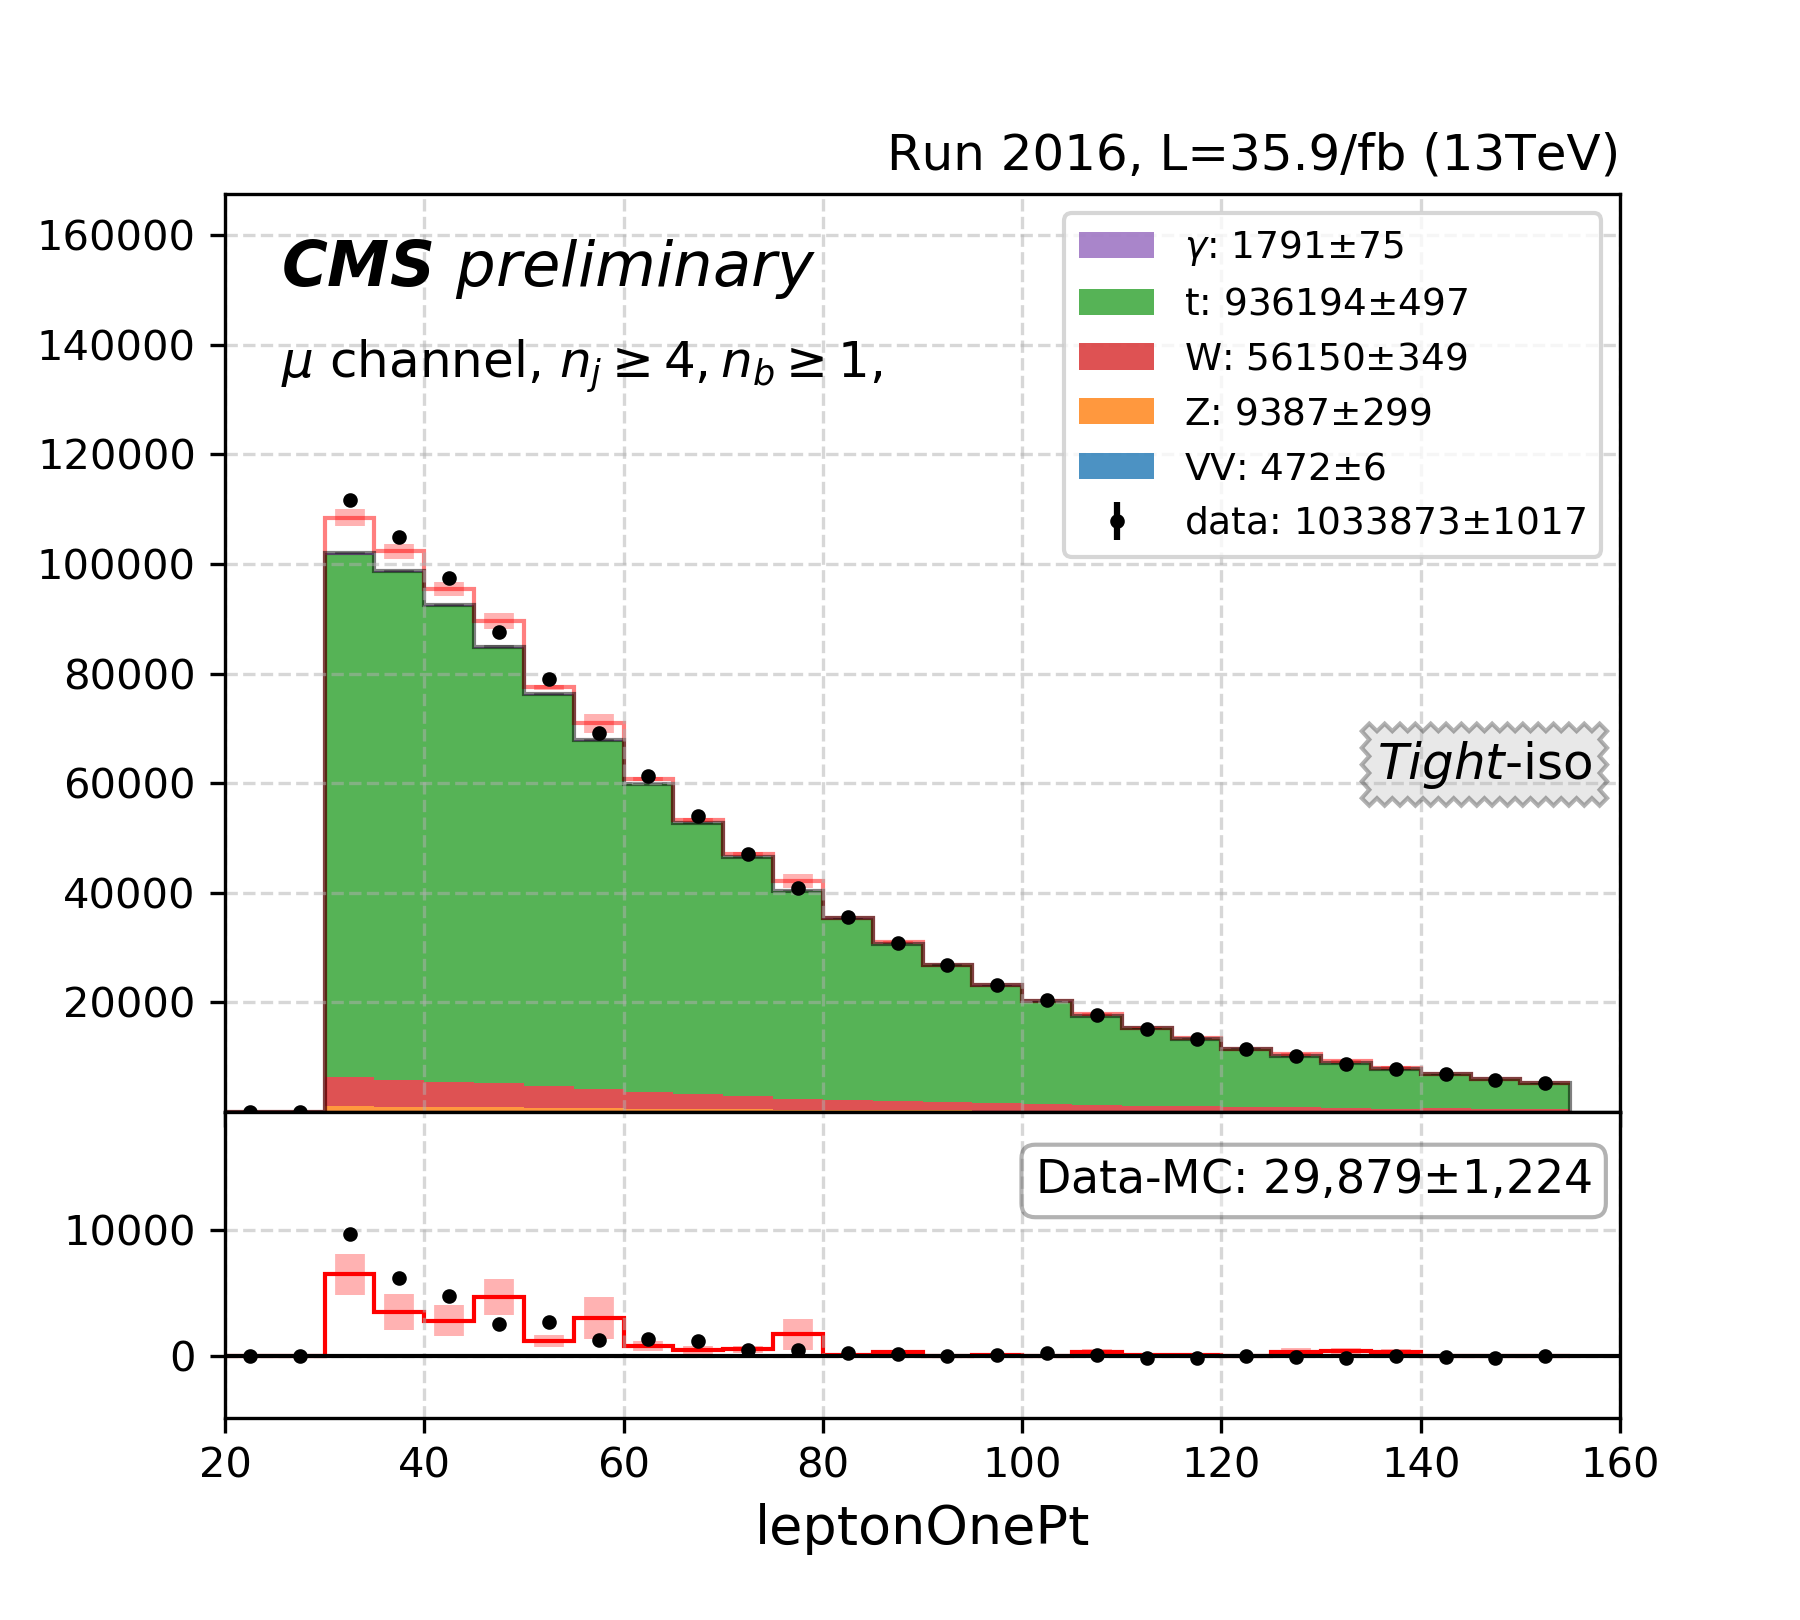
\includegraphics[width=0.24\textwidth]{chapters/Appendix/sectionQCD/figures/4j1b/mu_leptonOnePt_True_mcqcd.png}
    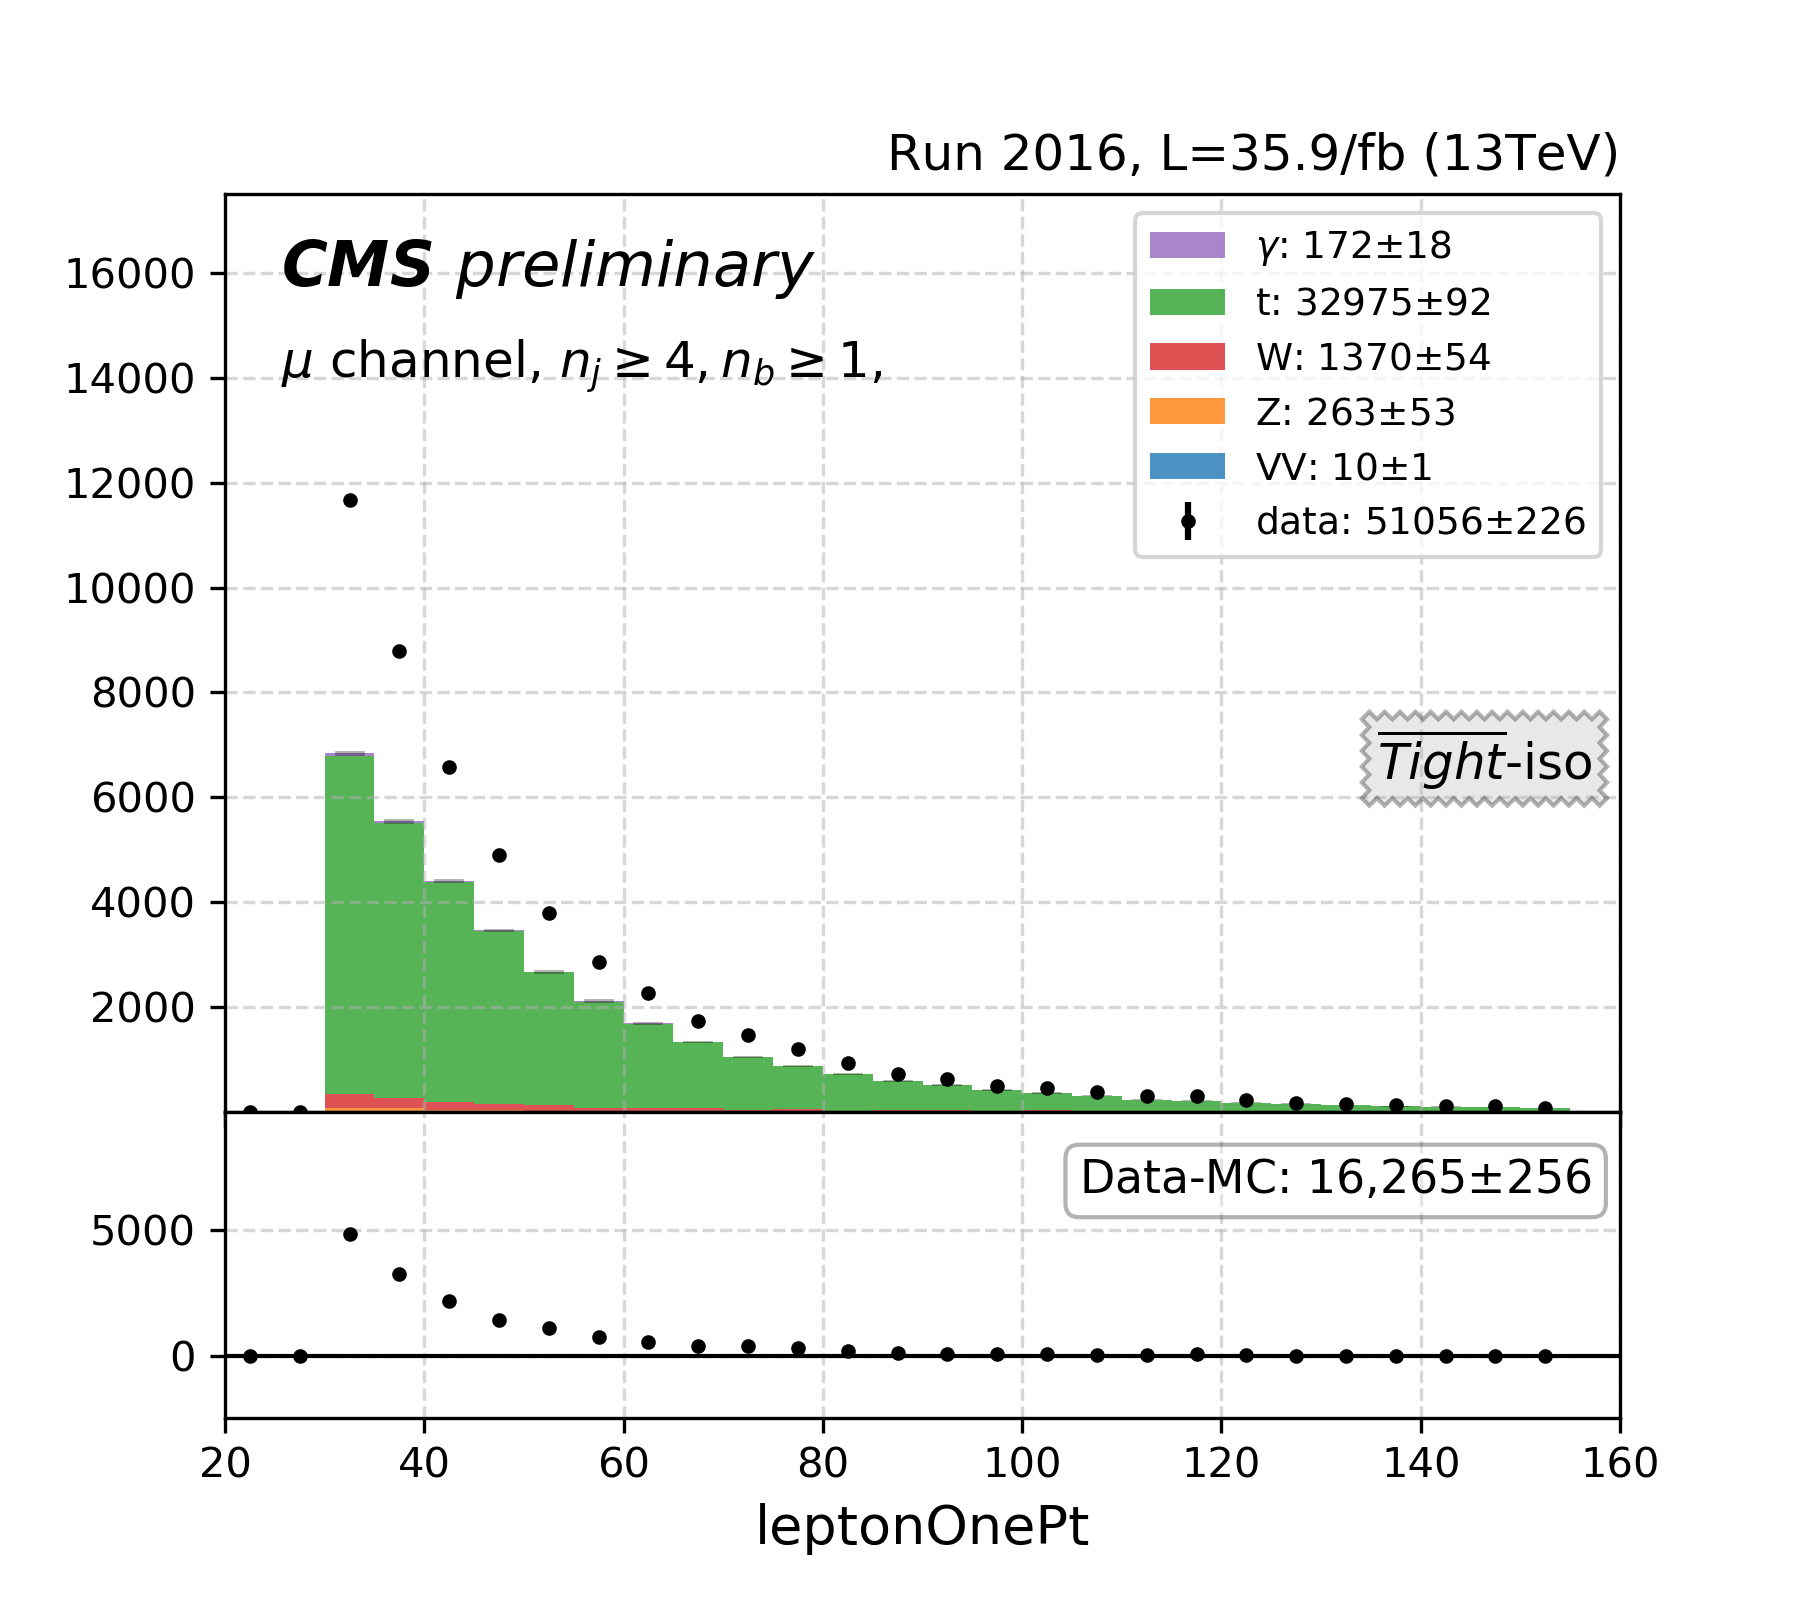
\includegraphics[width=0.24\textwidth]{chapters/Appendix/sectionQCD/figures/4j1b/mu_leptonOnePt_False.png}
    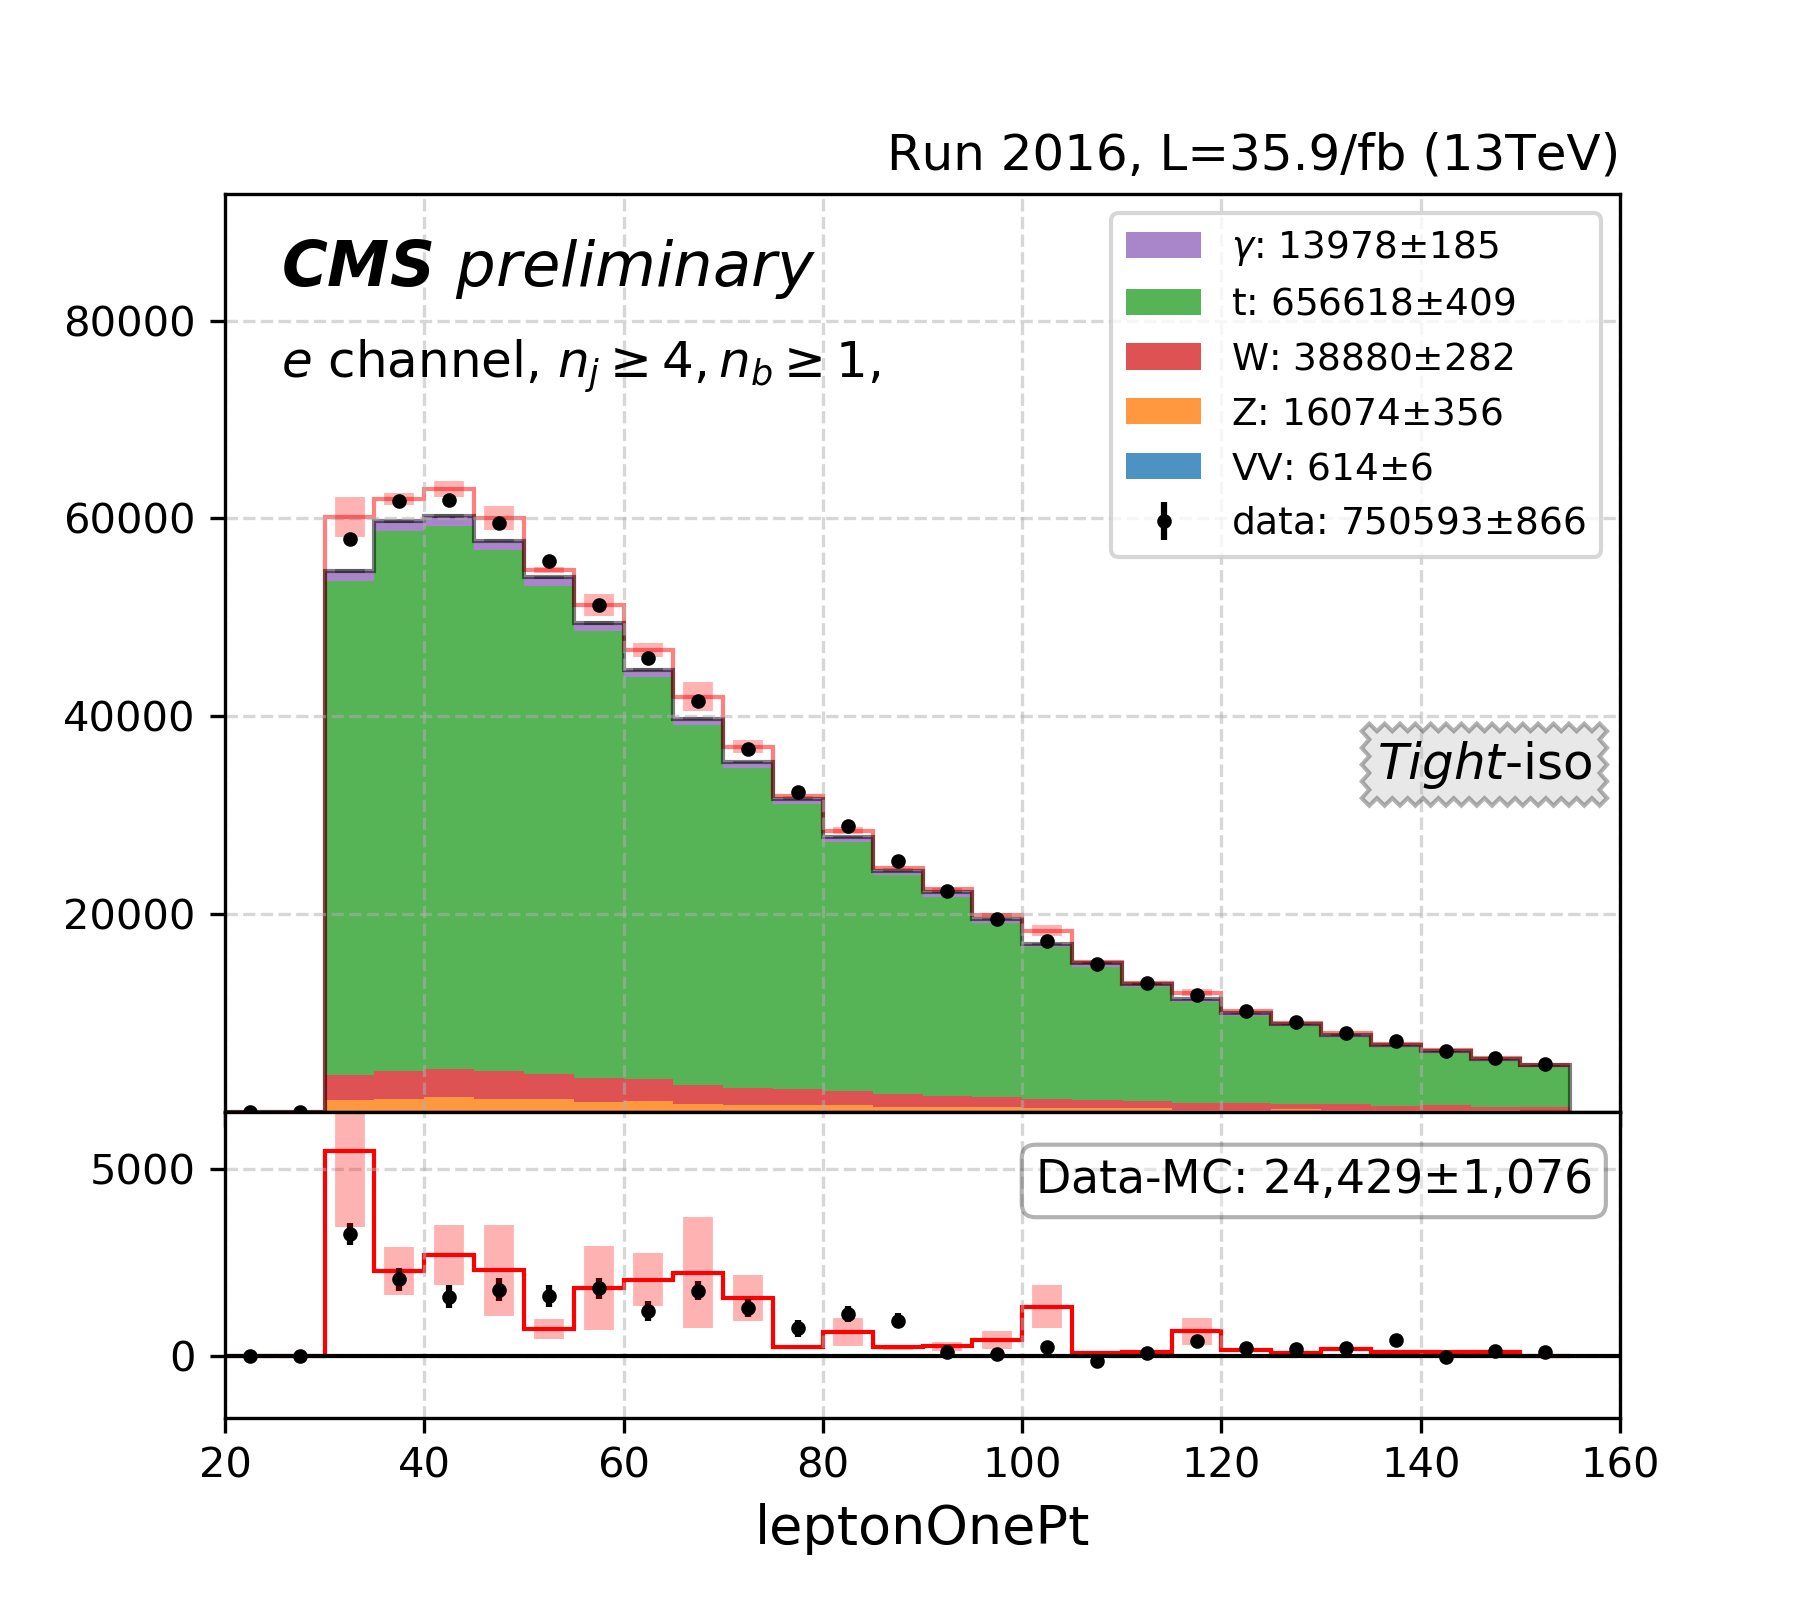
\includegraphics[width=0.24\textwidth]{chapters/Appendix/sectionQCD/figures/4j1b/e_leptonOnePt_True_mcqcd.png}
    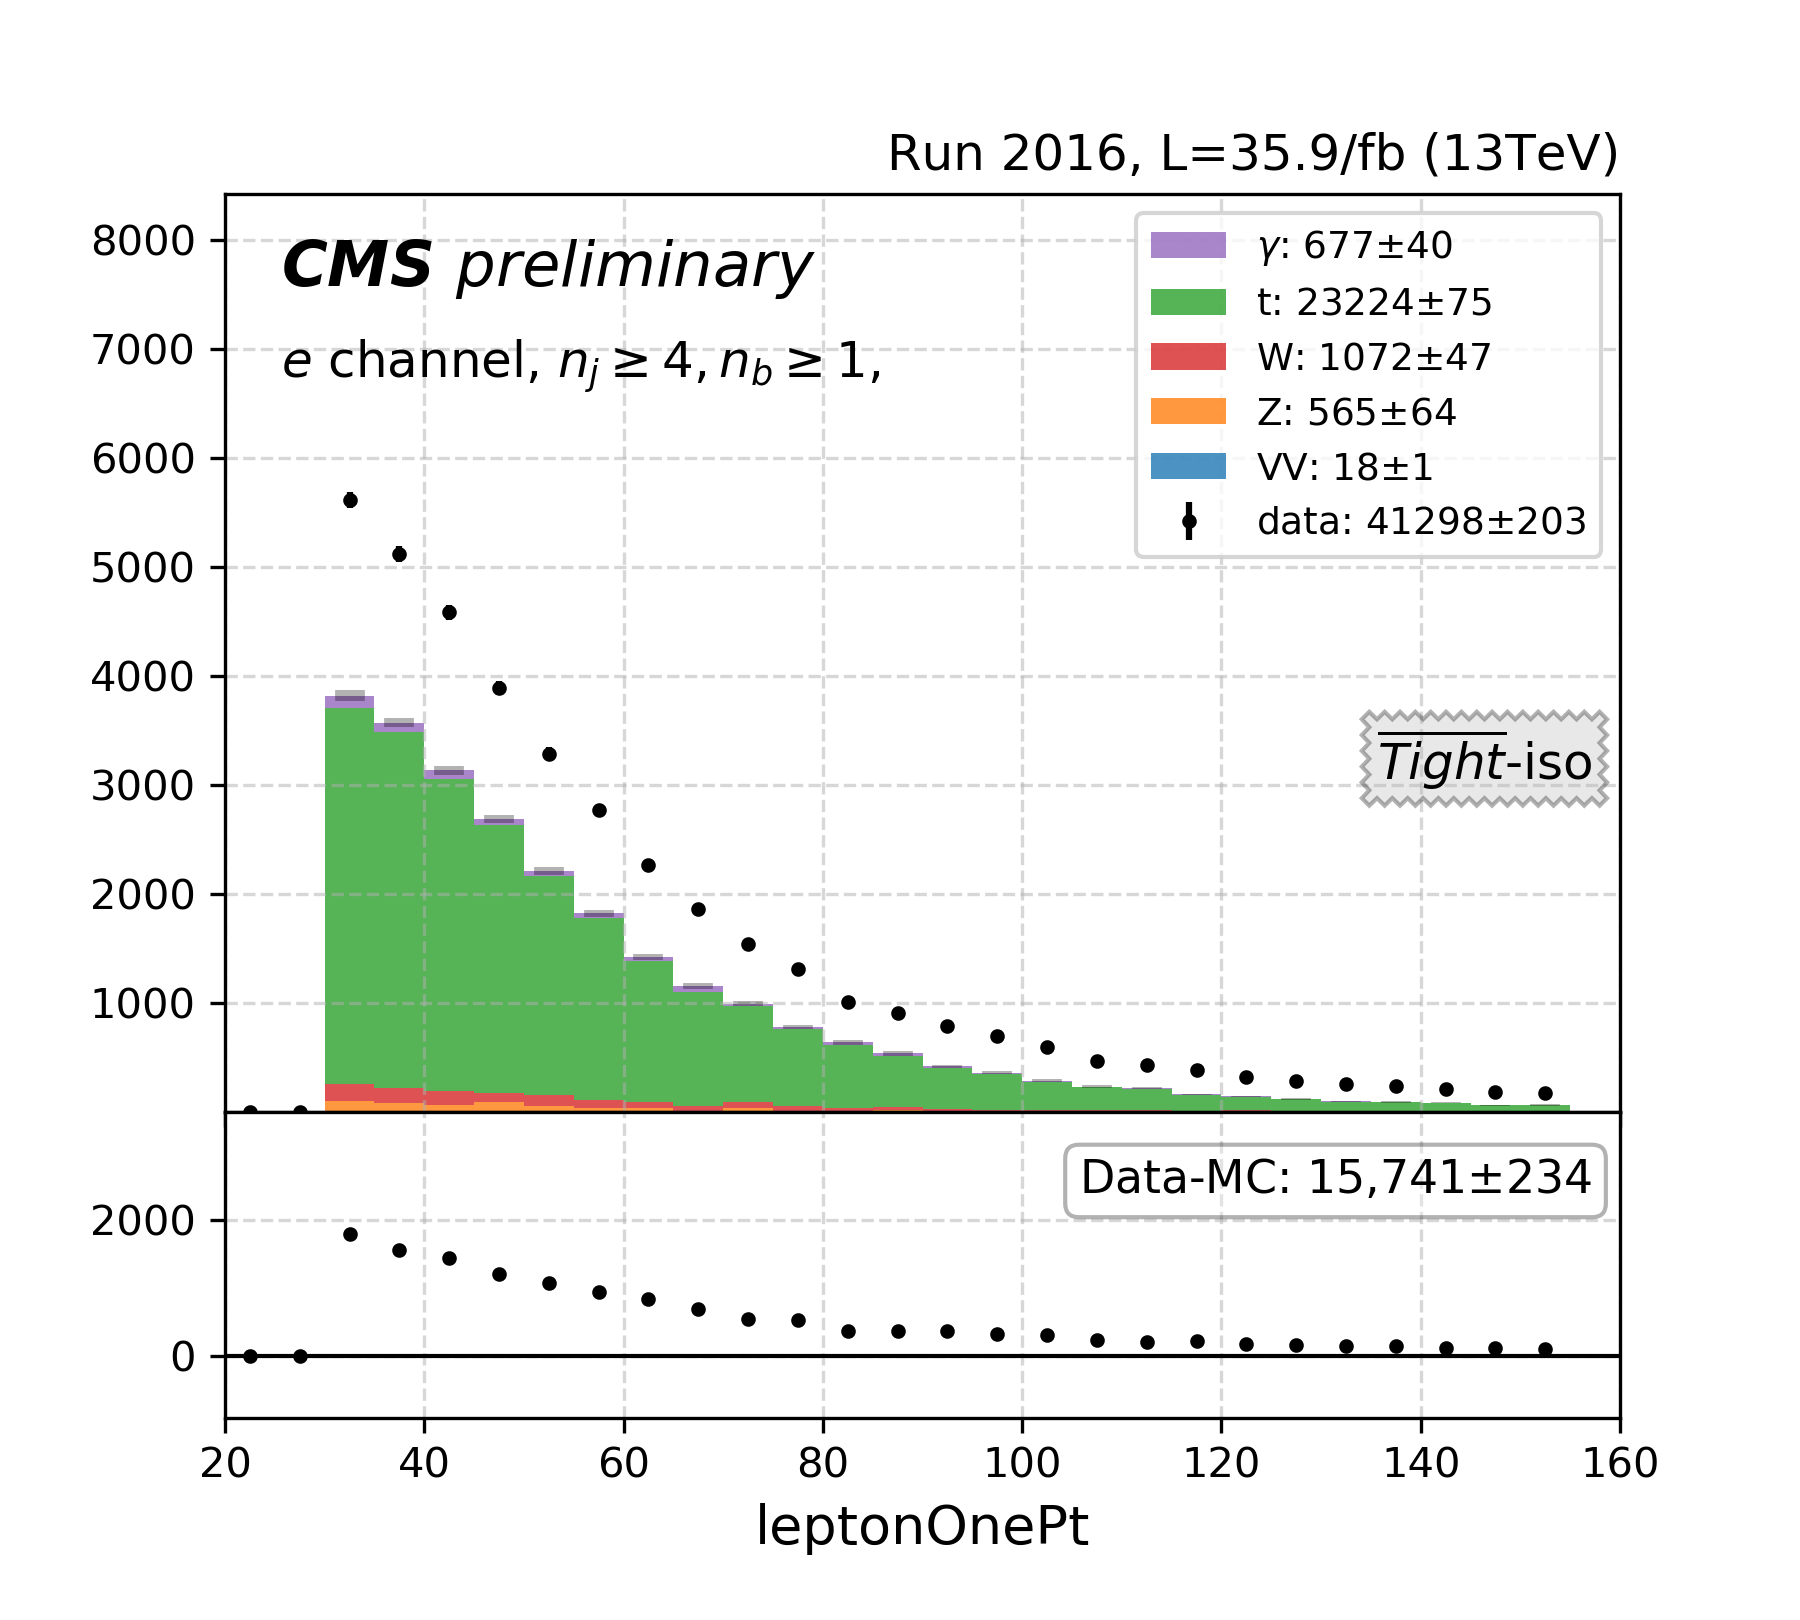
\includegraphics[width=0.24\textwidth]{chapters/Appendix/sectionQCD/figures/4j1b/e_leptonOnePt_False.png}
    
    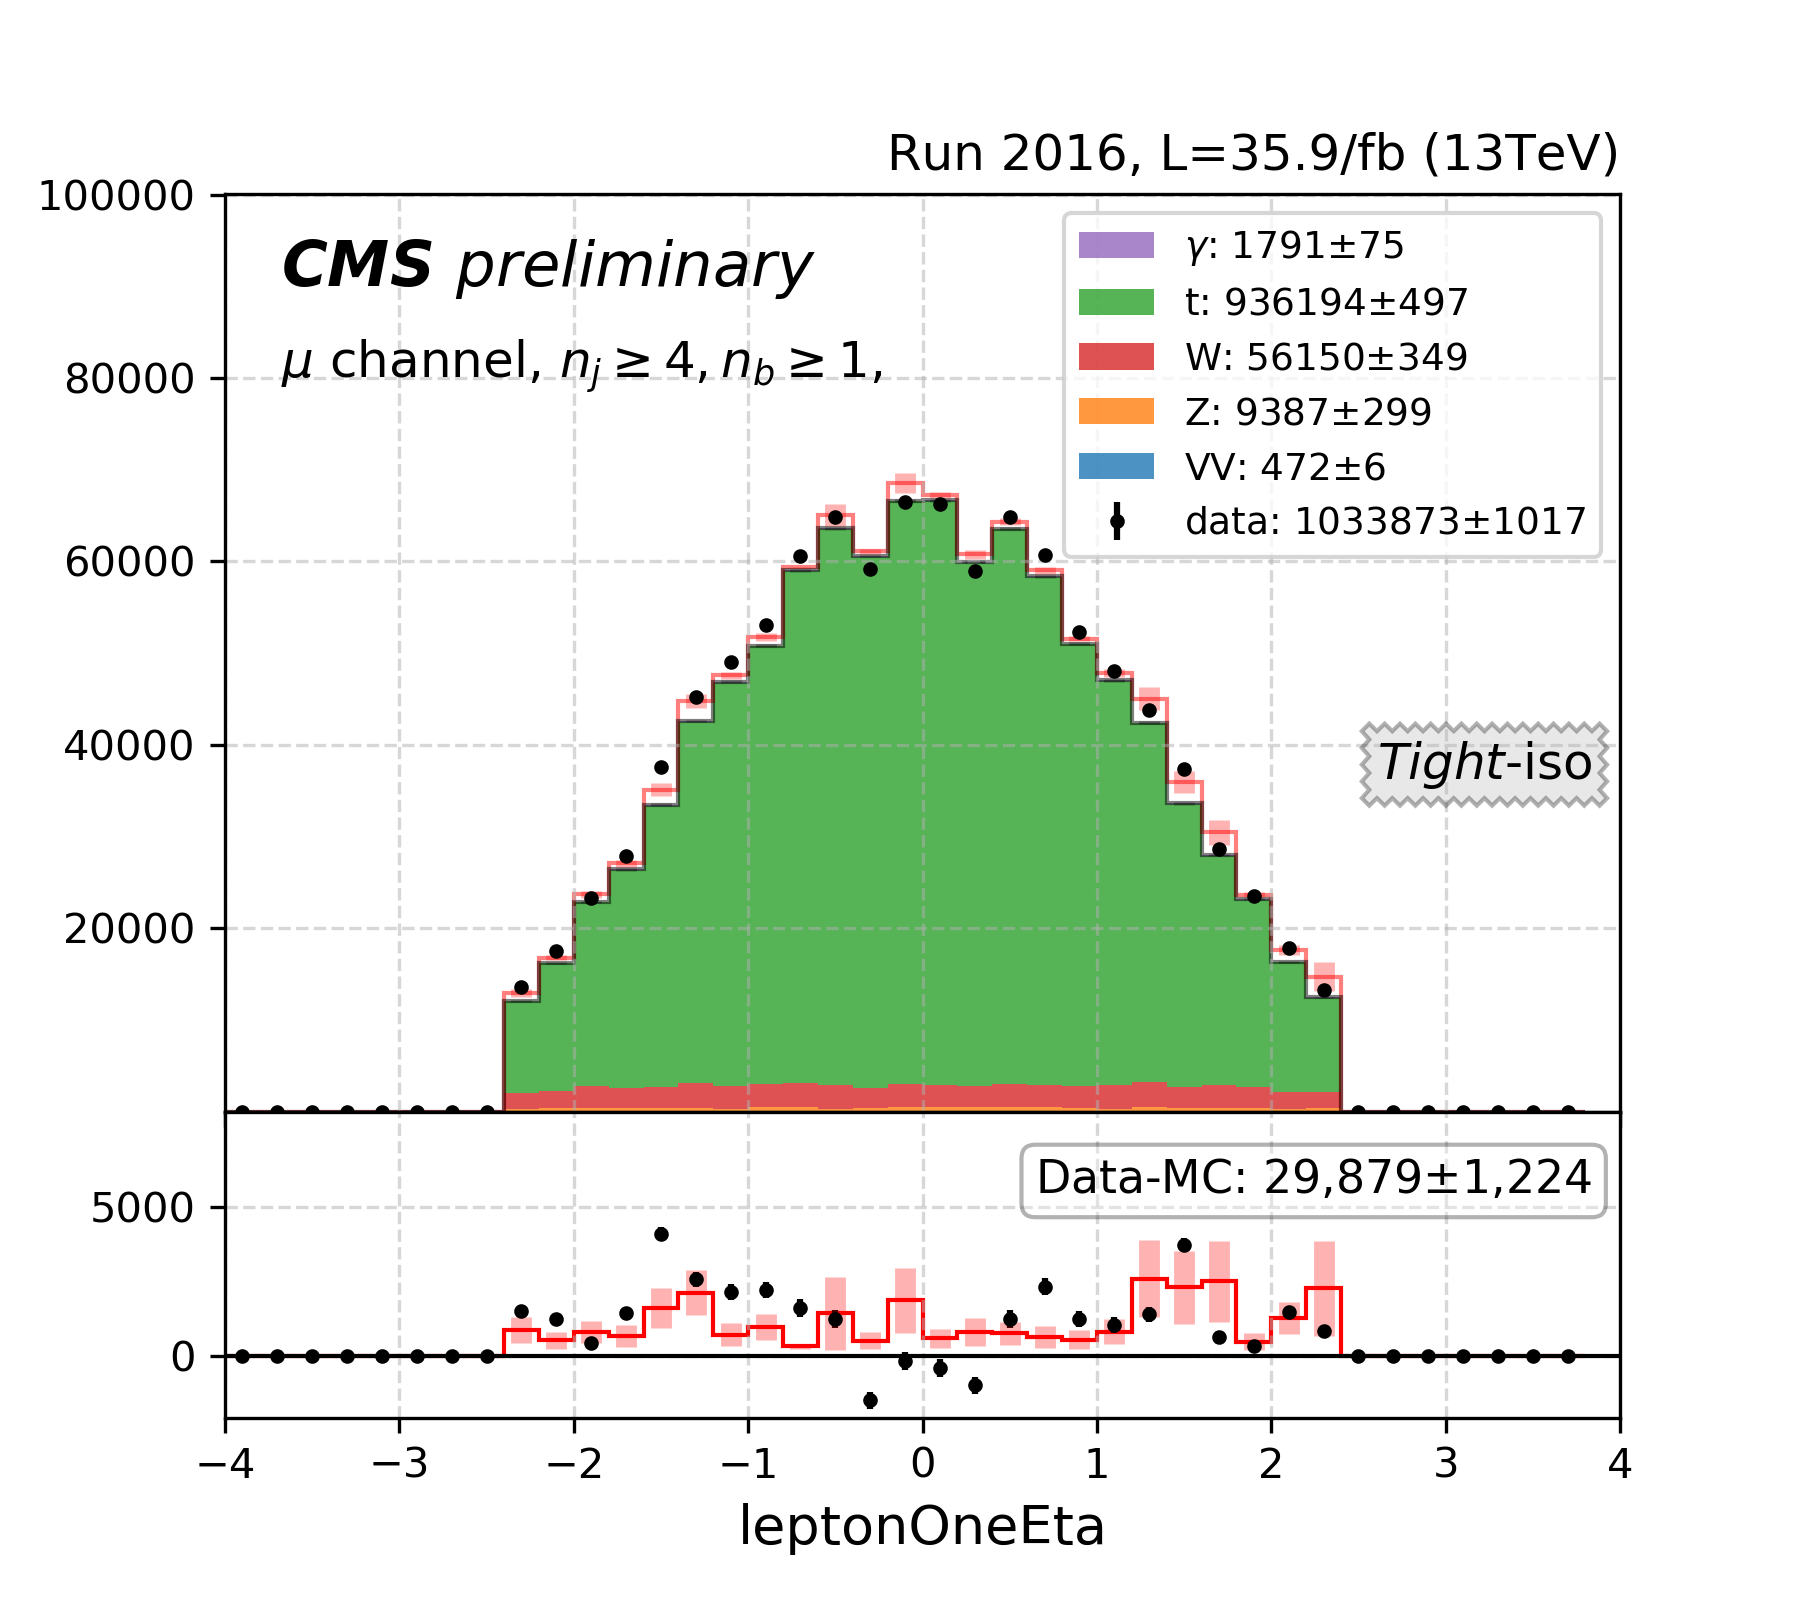
\includegraphics[width=0.24\textwidth]{chapters/Appendix/sectionQCD/figures/4j1b/mu_leptonOneEta_True_mcqcd.png}
    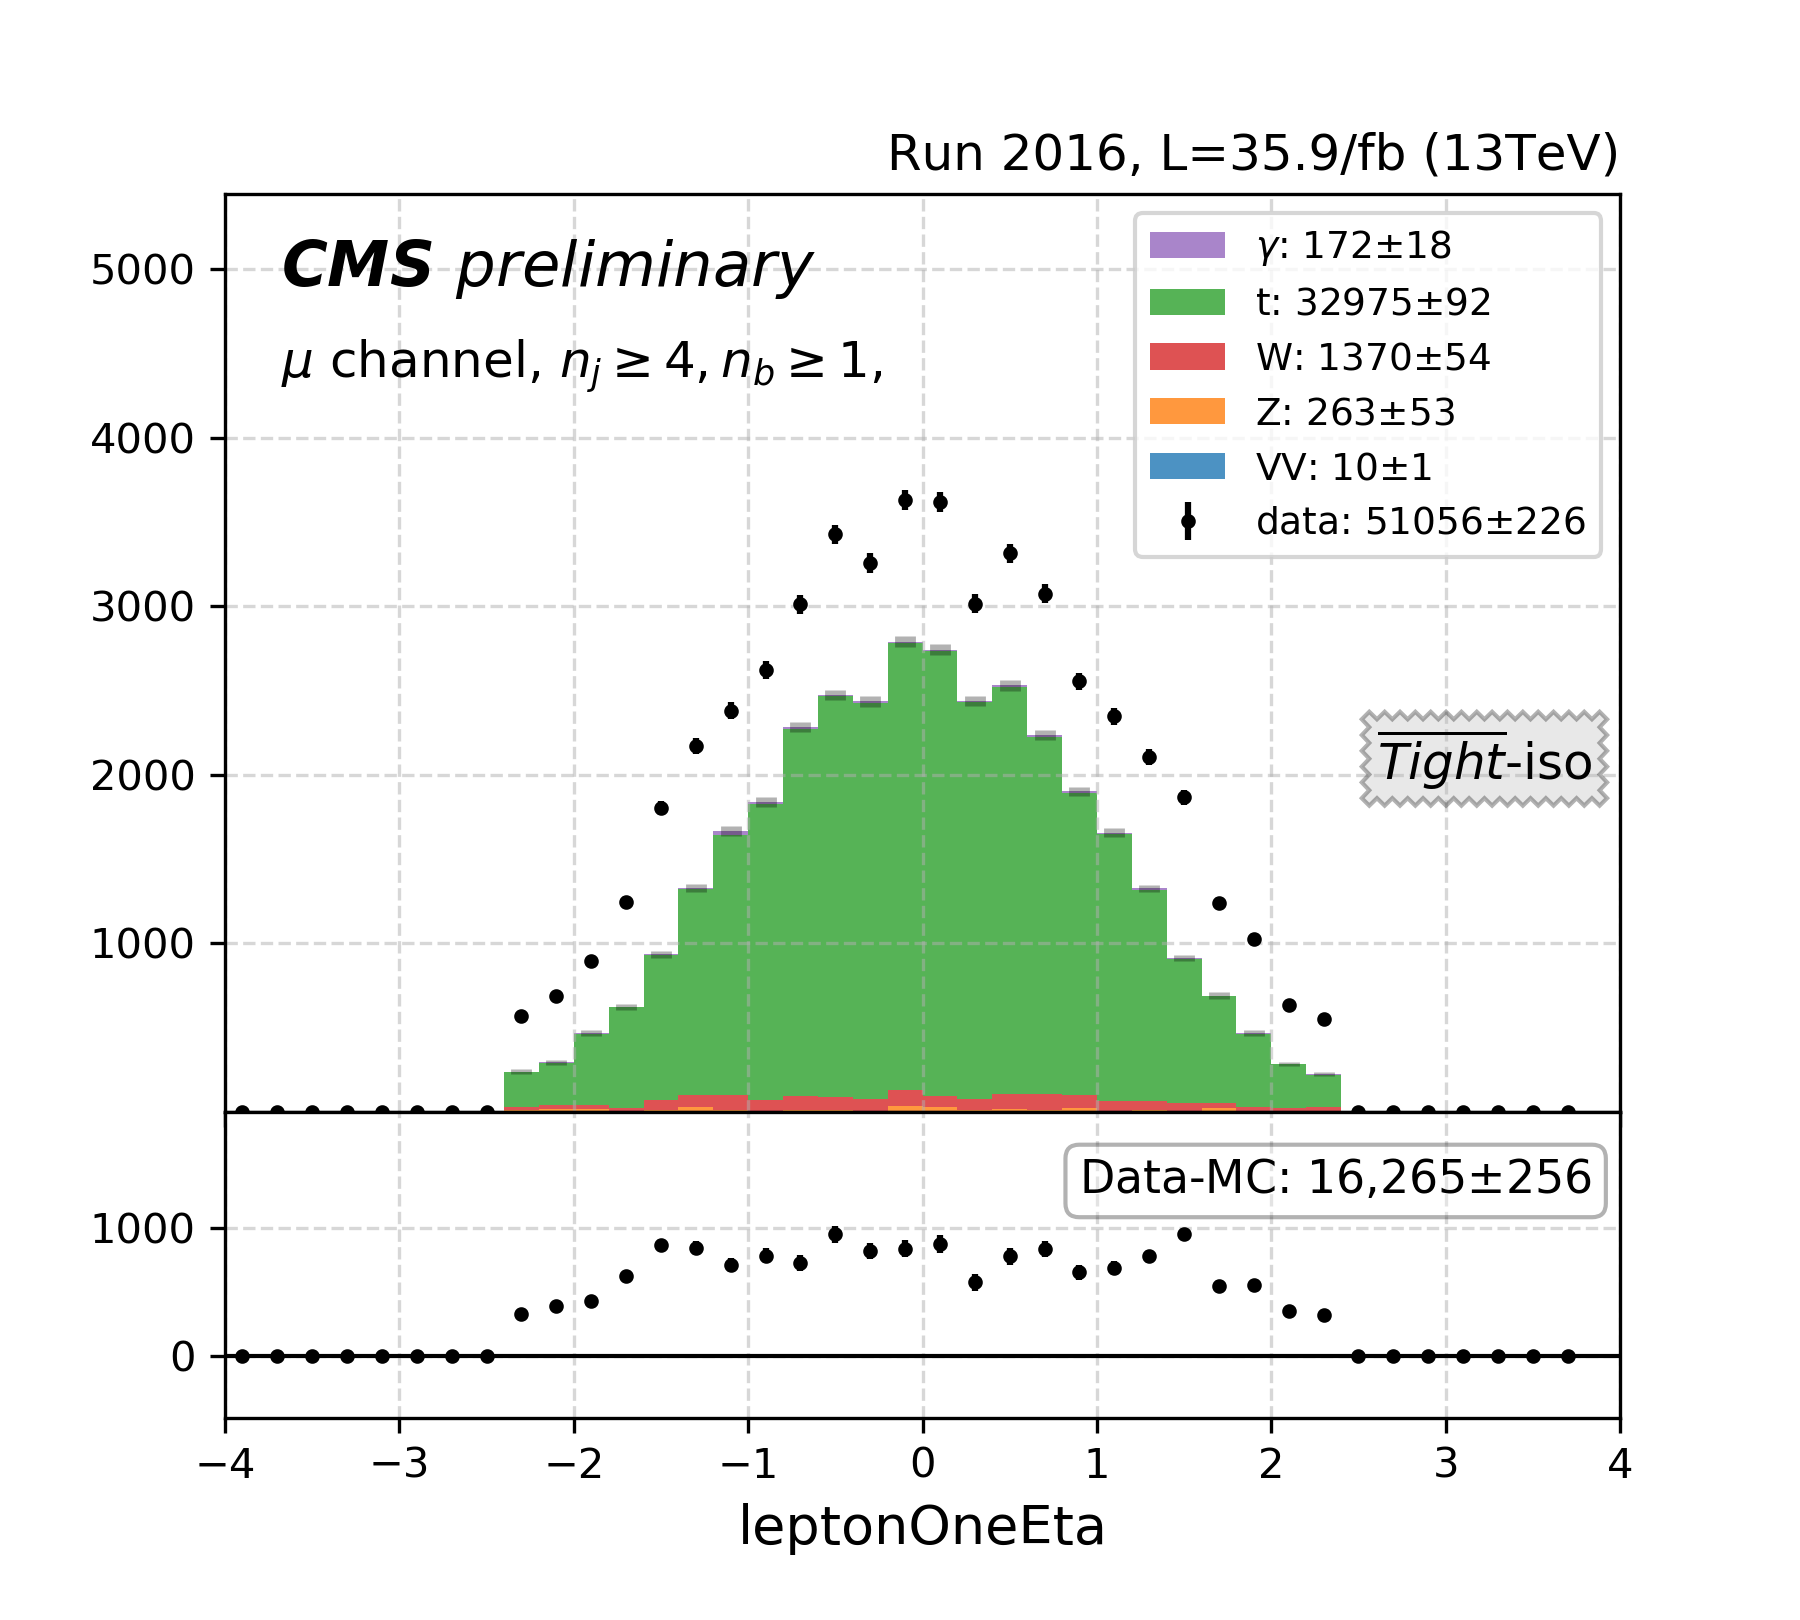
\includegraphics[width=0.24\textwidth]{chapters/Appendix/sectionQCD/figures/4j1b/mu_leptonOneEta_False.png}
    \includegraphics[width=0.24\textwidth]{chapters/Appendix/sectionQCD/figures/4j1b/e_leptonOneEta_True_mcqcd.png}
    \includegraphics[width=0.24\textwidth]{chapters/Appendix/sectionQCD/figures/4j1b/e_leptonOneEta_False.png}
    
    \includegraphics[width=0.24\textwidth]{chapters/Appendix/sectionQCD/figures/4j1b/mu_nJets_True_mcqcd.png}
    \includegraphics[width=0.24\textwidth]{chapters/Appendix/sectionQCD/figures/4j1b/mu_nJets_False.png}
    \includegraphics[width=0.24\textwidth]{chapters/Appendix/sectionQCD/figures/4j1b/e_nJets_True_mcqcd.png}
    \includegraphics[width=0.24\textwidth]{chapters/Appendix/sectionQCD/figures/4j1b/e_nJets_False.png}
    
    \includegraphics[width=0.24\textwidth]{chapters/Appendix/sectionQCD/figures/4j1b/mu_nBJets_True_mcqcd.png}
    \includegraphics[width=0.24\textwidth]{chapters/Appendix/sectionQCD/figures/4j1b/mu_nBJets_False.png}
    \includegraphics[width=0.24\textwidth]{chapters/Appendix/sectionQCD/figures/4j1b/e_nBJets_True_mcqcd.png}
    \includegraphics[width=0.24\textwidth]{chapters/Appendix/sectionQCD/figures/4j1b/e_nBJets_False.png}
    

    \caption{The iso and anti-iso region of $\mu$+jet (left two columns) and $e$+jet (right two columns) channel 
    with $n_j\geq4,n_b\geq1$, the signal region.}
    \label{fig:appendix:4j1b}
\end{figure}
\FloatBarrier